\documentclass[hyperref=colorlinks]{beamer}
\mode<presentation>
\usetheme{iclpt}
\setbeamertemplate{navigation symbols}{}
\setbeamertemplate{headline}{
\begin{beamercolorbox}[leftskip=.2cm,rightskip=.2cm,topskip=.2cm,ht=1.1cm,dp=0.1cm,wd=\textwidth]{institute in head/foot}
  
\includegraphics[height=1cm]{icl.pdf}
  \hfill
  
\includegraphics[height=1cm]{../Pics/CMS-Color.pdf}
\end{beamercolorbox}
}
\setbeamertemplate{footline}{
\begin{beamercolorbox}[ht=.55cm,dp=0.4cm,wd=\textwidth,leftskip=.3cm]{author in head/foot}%
  \begin{minipage}[c]{5cm}%
    \usebeamerfont{author in head/foot}
    \insertshortauthor 
    \insertshorttitle
    \end{minipage}\hfill%
  \insertframenumber{} / \pageref{lastframe}
  \hfill
  \begin{minipage}{6cm}
    \hfill
  \end{minipage}
\end{beamercolorbox}%
}

\usepackage{color}
\usepackage{tabularx,colortbl}
\usepackage{graphicx}
\usepackage{pdfpages}
\usepackage{feynmp}
\DeclareGraphicsRule{*}{mps}{*}{}

\title{\vspace{-0.2cm} Control Plots}
%\subtitle{Paper - HIG-13-030, PASs: HIG-13-013, HIG-13-018, HIG-13-028 \vspace{-0.7cm}}
\author[P. Dunne]{\underline{P. Dunne} }%\\ on behalf of the H$\rightarrow$invisible analysis groups} % A.M. Magnan and A. Nikitenko Joao Pela with \\ R. Aggleton, J. Brooke: Bristol \\ C.Asawangtrakuldee, Q.Li: Peking \\ P. Srimanobhas: Chulalongkorn \\ S. Kumar, K. Mazumdar: Mumbai}
\titlegraphic{
  \vspace{-0.7cm}
  %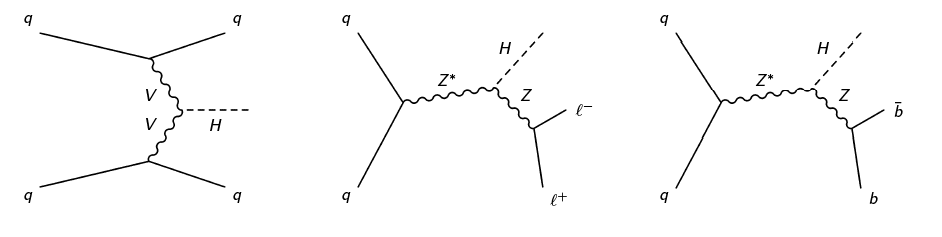
\includegraphics[width=\textwidth]{TalkPics/invcomb021213/feyndiags}
%% \begin{fmfgraph*}(100,70)
%%         \fmfleft{i1,i2}
%%         \fmfright{o1,o2,o3}
%%         \fmf{fermion}{i1,v1,o1}
%%         \fmf{fermion}{i2,v2,o3}
%%         \fmf{phantom,tension=4/5}{v1,v2}
%%         \fmffreeze
%%         \fmf{photon,label=$W,,Z$}{v1,v3}
%%         \fmf{photon,label=$W,,Z$}{v2,v3}
%%         \fmf{dashes}{v3,o2}
%%         \fmflabel{$q$}{i1}
%%         \fmflabel{$q$}{i2}
%%         \fmflabel{$q$}{o1}
%%         \fmflabel{$q$}{o3}
%%         \fmflabel{$H$}{o2}
%%       \end{fmfgraph*}
}
\date{}
\begin{document}
\begin{fmffile}{hig1330approvalfeynmandiags}

%TITLE PAGE
\section{Title}
\begin{frame}
  \titlepage
  
\end{frame}

%OUTLINE
\begin{frame}
  \frametitle{Overview}
  \begin{block}{}
    \scriptsize
    \begin{itemize}
    \item Pre-selection has been reoptimised
    \item First focus on agreement in control regions
    \item[-] This minimises effect of mismodelled QCD
    \item Have seen previously significant top contribution to W control regions
    \item[-] Investigated $m_{T}$ as a means to discriminate
    \item Initially just varied met significance and leading jets-metnomu min$\Delta\phi$ cuts
    \item[-] Tried adding all jets $p_{T}>30$ to the min$\Delta\phi$ calculation
    \end{itemize}
  \end{block}
\end{frame}

\begin{frame}
  \frametitle{New Control Plots}
    \begin{block}{}
      \scriptsize
      \begin{itemize}
      \item Cuts applied in all following plots are:
      \item[-] metnomu$>90$ $jet_{1} p_{t}>50$, $\Delta\eta_{jj}>3.6$, metnomu\_significance$>3$, $jet_{1,2} \eta <4.7$, $jet_{1}\eta\cdot jet_{2}\eta<0,m_{jj}>=800,jet_{2} p_{T}>40$
      \item[-] met, $jet2 p_{T}$ and $m_{jj}$ cuts chosen to be above highest trigger threshold and at at least 50\% efficiency for run D trigger 
      \end{itemize}
    \end{block}
\end{frame}

\begin{frame}
%DISCUSSION OF MT IN W REGIONS AND ACTION IN WTAU
  \frametitle{mT in W control regions}
  \begin{block}{}
    \scriptsize
    \begin{itemize}
    \item Top contamination of W regions is up to 30\% in some regions
    \end{itemize}
  \end{block}
  \begin{columns}
    \column{.5\textwidth}
    \begin{block}{enu}
      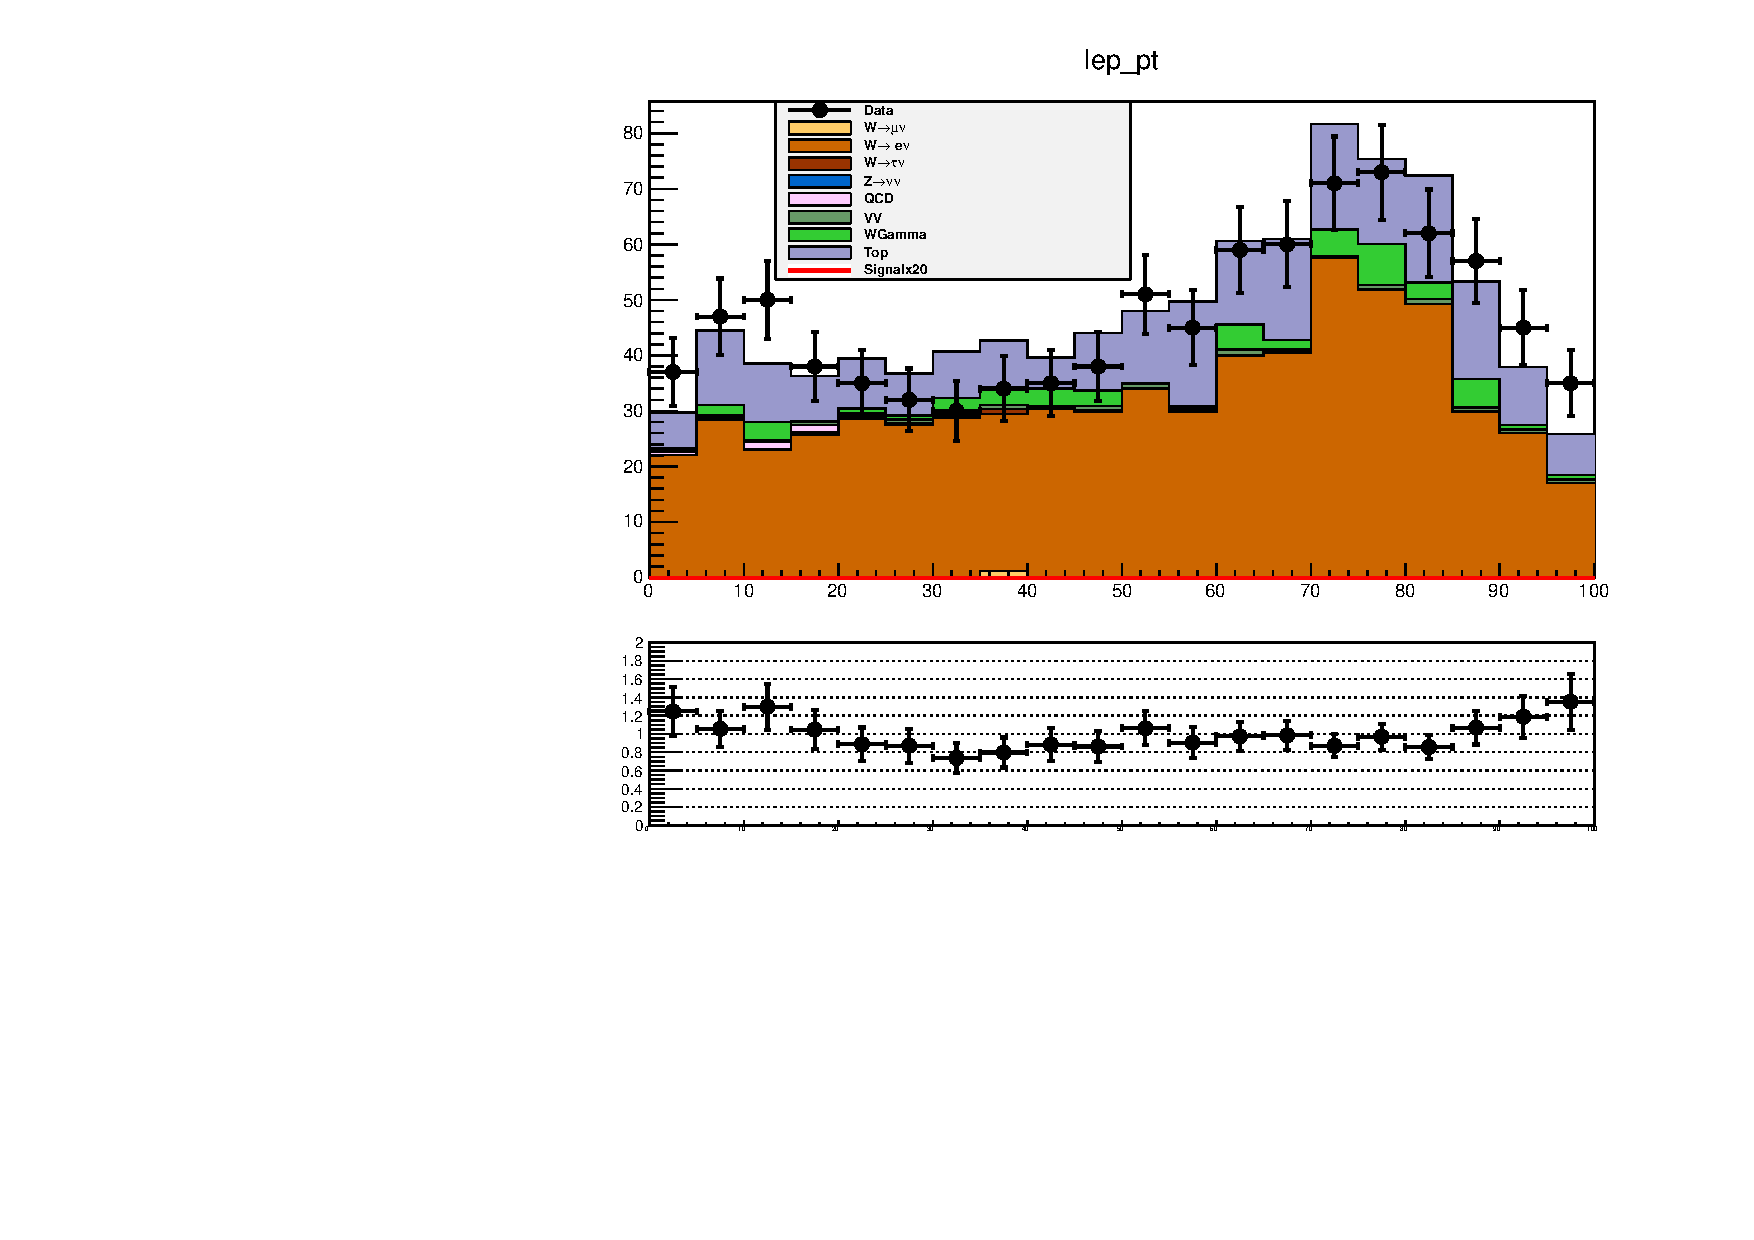
\includegraphics[width=\textwidth]{TalkPics/contplotsandpresel150914/oldpreselmts/enumt.pdf}
    \end{block}
    \column{.5\textwidth}
    \begin{block}{munu}
      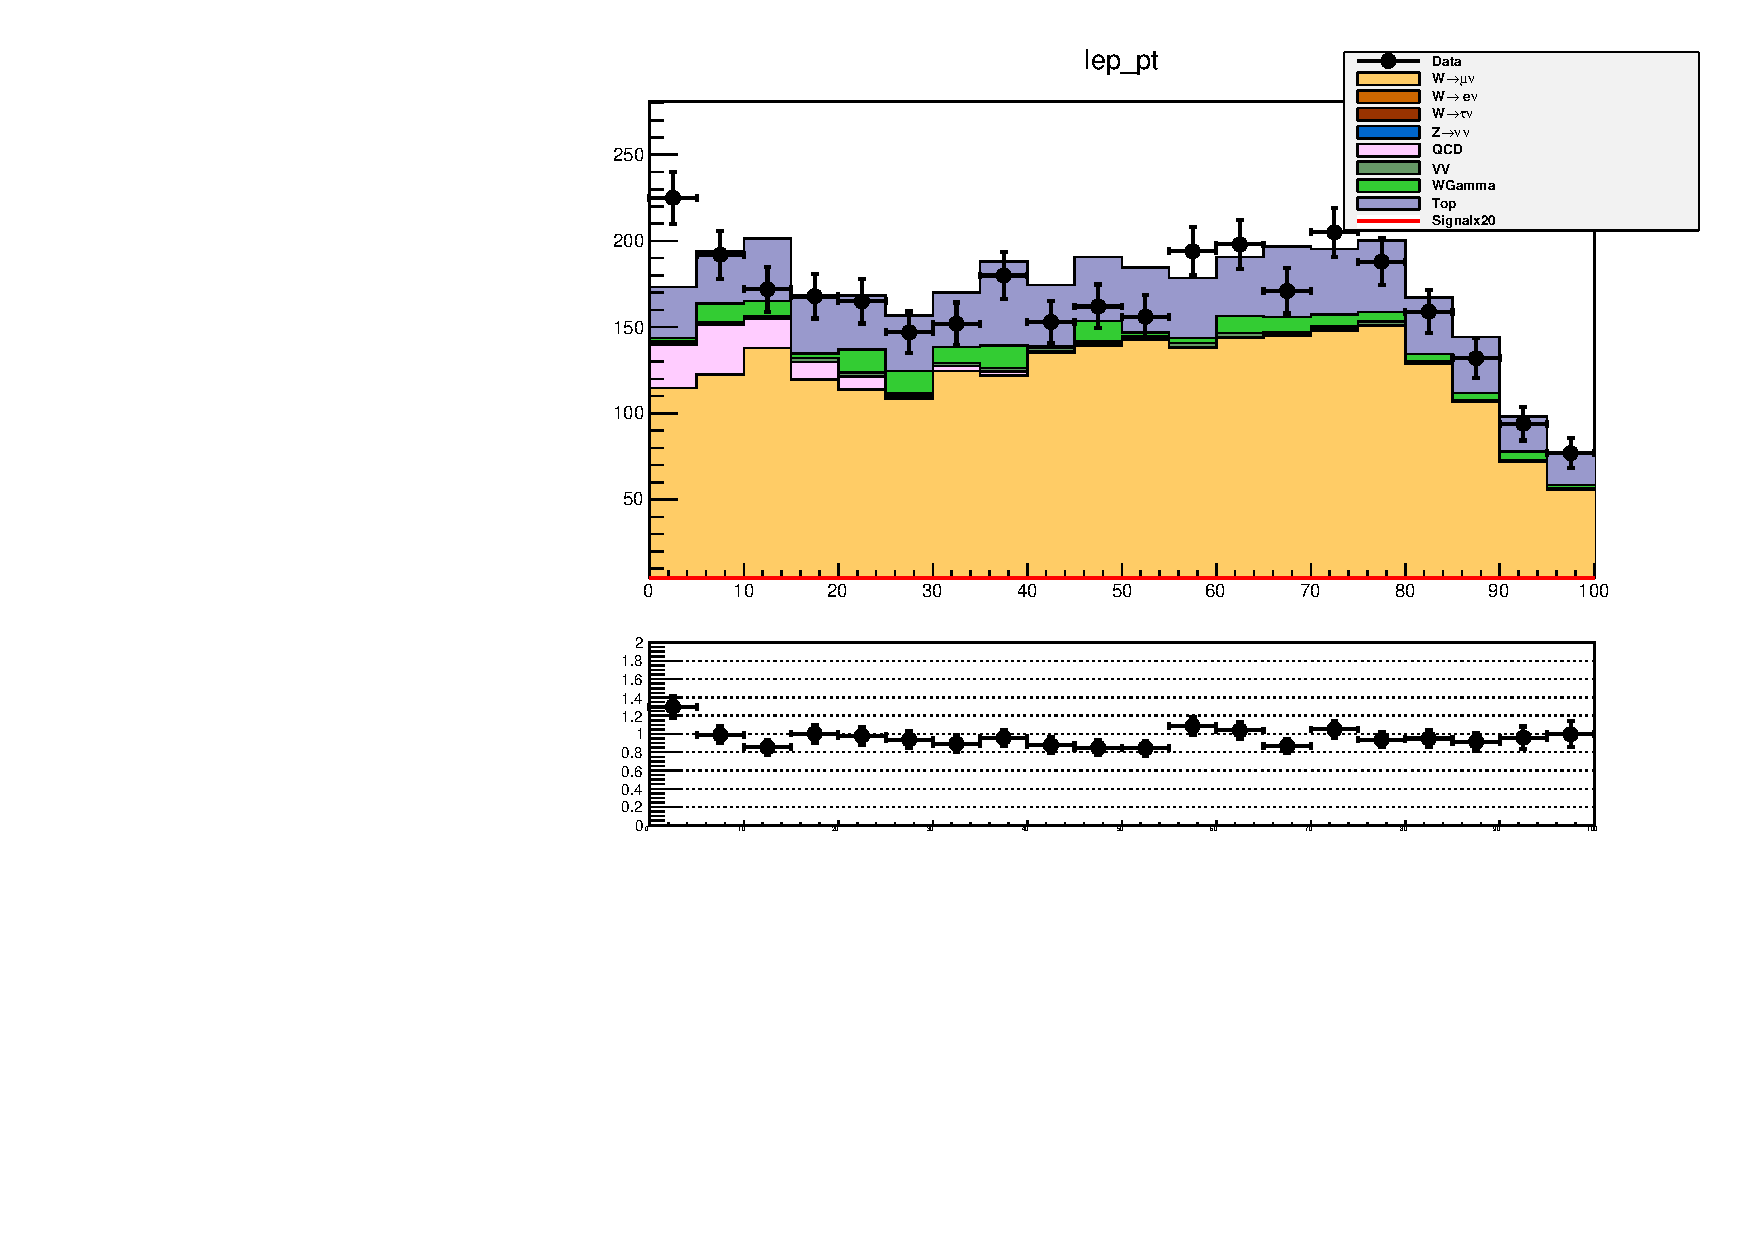
\includegraphics[width=\textwidth]{TalkPics/contplotsandpresel150914/oldpreselmts/munumt.pdf}
    \end{block}

  \end{columns}
\end{frame}

\begin{frame}
%DISCUSSION OF MT IN W REGIONS AND ACTION IN WTAU
  \frametitle{mT in W control regions}
  \begin{columns}
    \column{.5\textwidth}
    \begin{block}{taunu}
      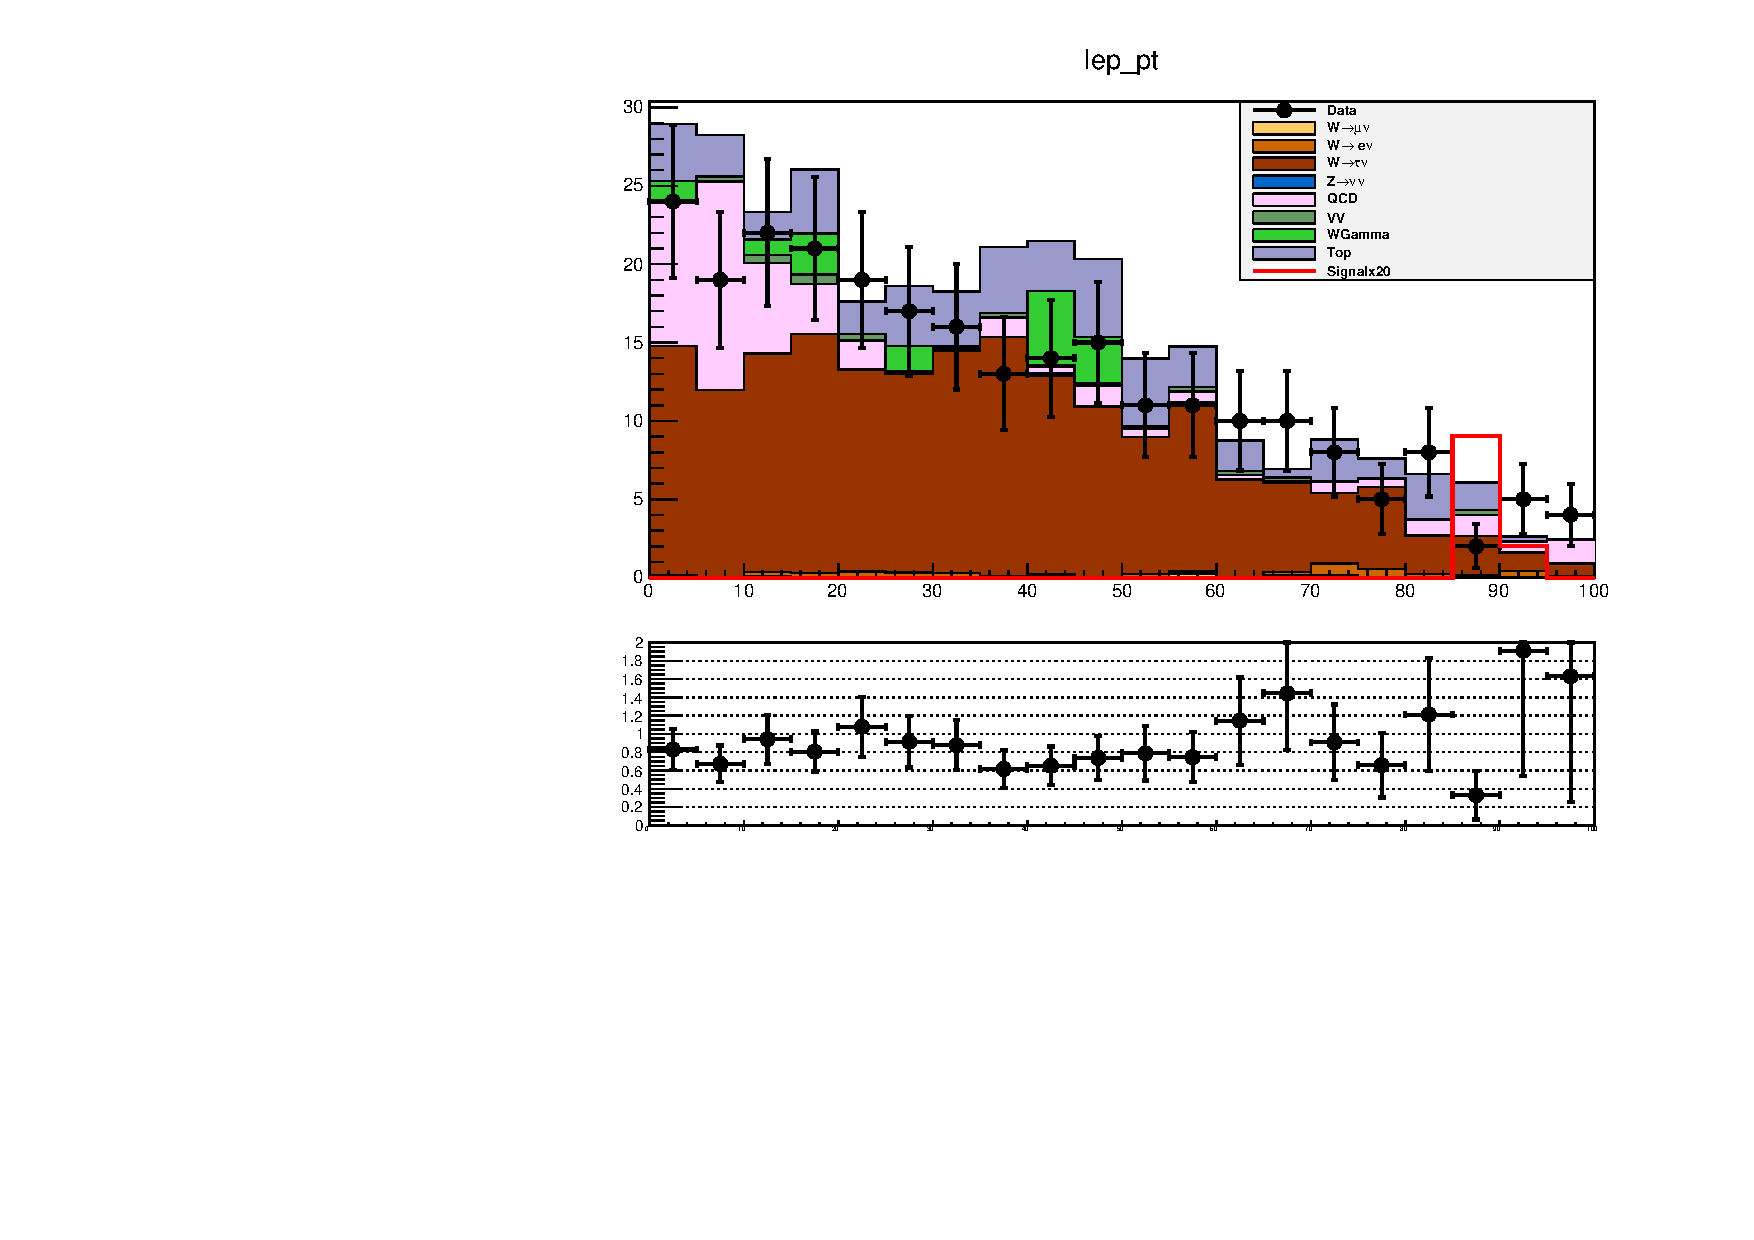
\includegraphics[width=\textwidth]{TalkPics/contplotsandpresel150914/oldpreselmts/taunumt.pdf}
    \end{block}
  \end{columns}
  \begin{block}{}
    \scriptsize
    \begin{itemize}
    \item mt doesn't seem to give any discrimination against top
    \item For tau does allow removal of QCD contamination
    \item[-] Have added an mt$>20 GeV$ cut on tau control region
    \end{itemize}
  \end{block}
\end{frame}

\begin{frame}
  %LEADINGJETMETDPHI AND ALLJETSMETDPHI DISTRIBUTIONS
  \frametitle{$\Delta\phi(j,met)$ variables - intro}
  \begin{block}{}
    \scriptsize
    \begin{itemize}
    \item n.b. scale is different between plots
    \item Version with all jets $p_{T}>30$ GeV has better data MC agreement
    \item QCD almost all moves to low values of variable
    \end{itemize}
  \end{block}
  \begin{columns}
    \column{.5\textwidth}
    \begin{block}{\scriptsize $min(\Delta\phi(j_{1,2},metnomu))$}
      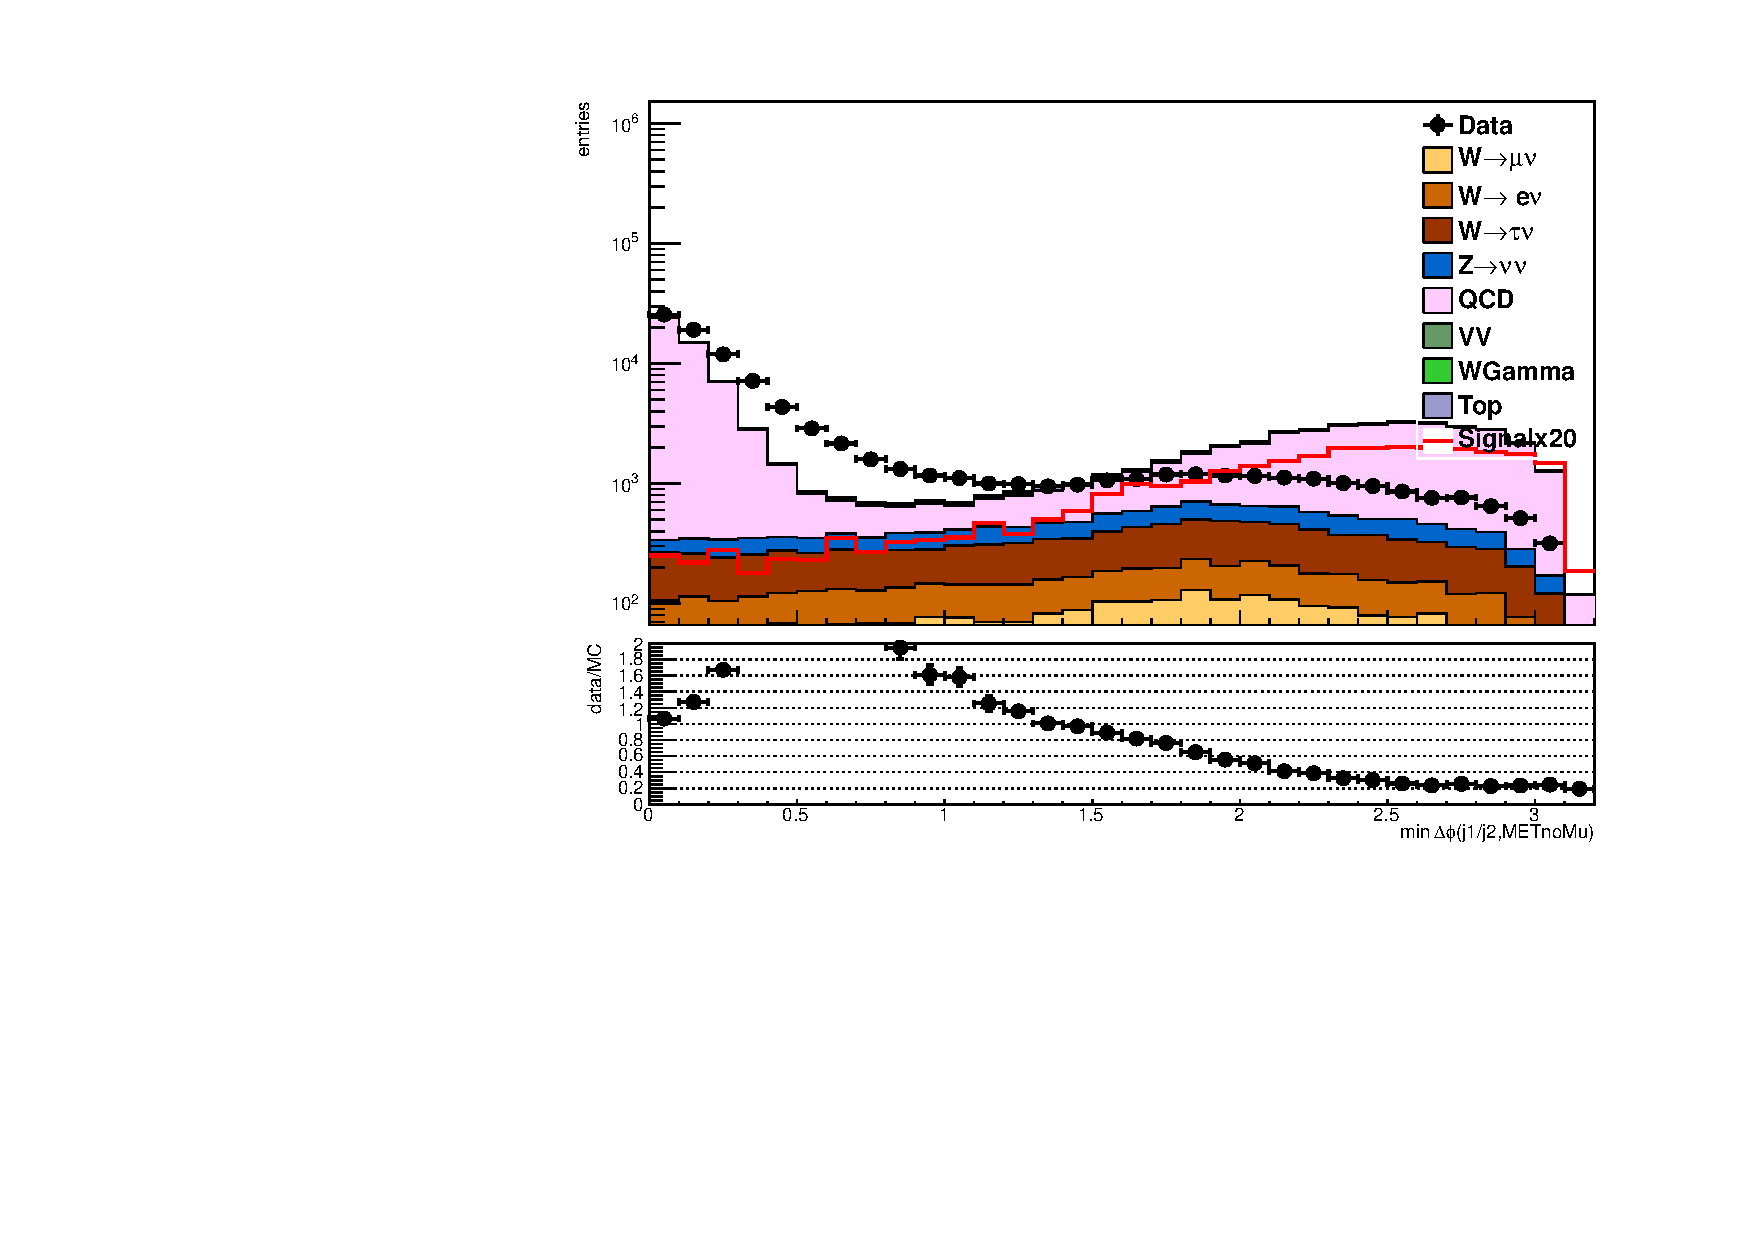
\includegraphics[width=\textwidth]{TalkPics/contplotsandpresel150914/leadingjetsmetnomudphinocut.pdf}
    \end{block}
    \column{.5\textwidth}
    \begin{block}{\scriptsize $min(\Delta\phi(all\,j(p_{T}>30),metnomu))$}
      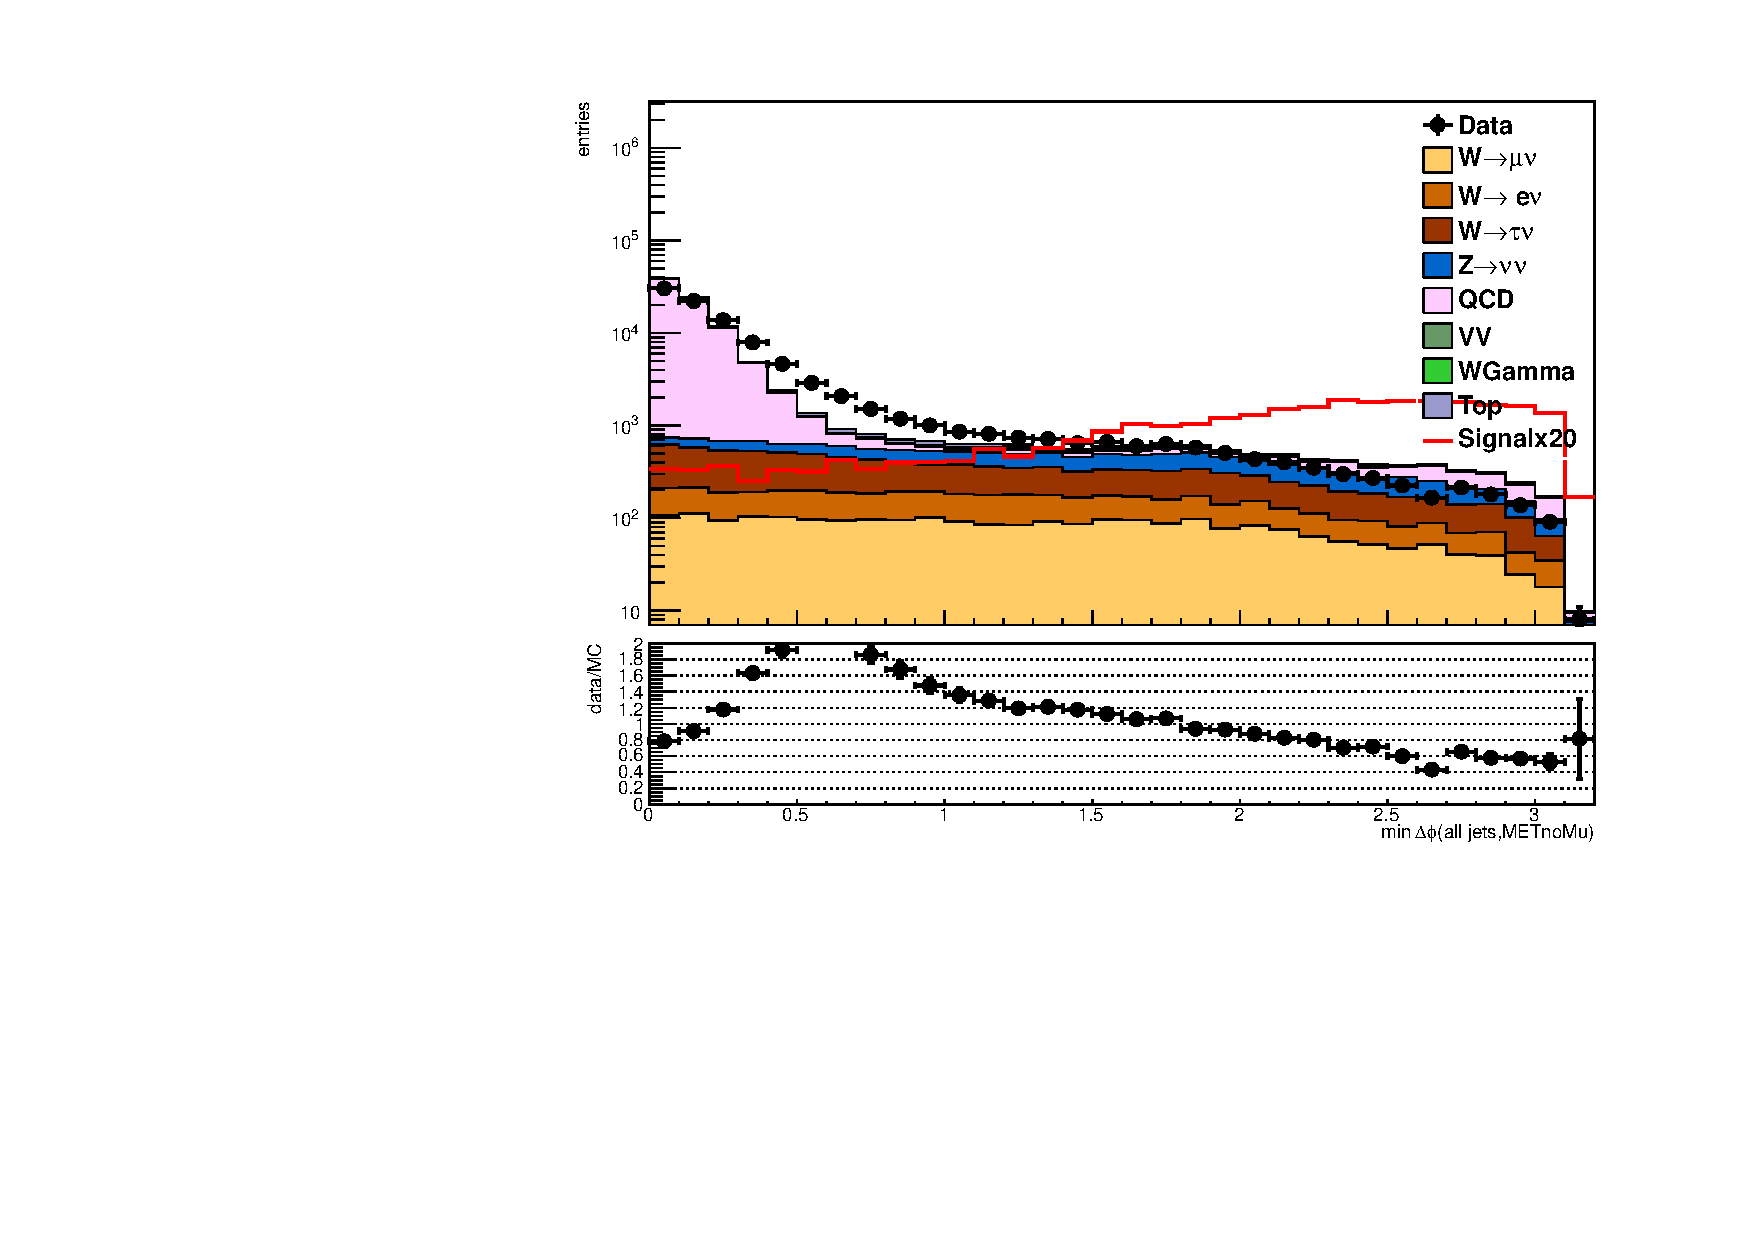
\includegraphics[width=\textwidth]{TalkPics/contplotsandpresel150914/alljetsmetnomudphinocut.pdf}
    \end{block}

  \end{columns}
\end{frame}

\begin{frame}
  %SUMMARY TABLES WITH CUTS
  \frametitle{$\Delta\phi(j,met)$ variables - cut efficiency}
  \begin{columns}
    \column{1.1\textwidth}
  \begin{block}{}
    \scriptsize
    \begin{tabular}{l||c|c|c|c||c|c|c}
      Process & no cut & $j_{1,2}>0.5$ & $j_{1,2}>1.0$ & $j_{1,2}>1.5$ & all$>0.5$ & all$>1.0$ & all$>1.5$\\
      \hline
      wel & 2187  &1854 &1477 &1073 &1682 &1185 &727 \\
      wmu & 2445  &2087 &1697 &1243 &1889 &1379 &901  \\
      wtau & 5618 &3392 &2391 &1653 &2755 &1763 &1482  \\
      zvv & 3924  &3425 &2977 &2086 &3170 &2559 &1556  \\
      qcd & 80400 &16088 &9488 &{\color{red}7363 }&7079 &{\color{red}1597} &489  \\
      vv & 133    &119 &103 & 88 &101 &75 & 55 \\
      wg & 421    &349 &306 & 248 &292 &209 & 135 \\
      top & 1349  &1180 &1006 &795 &764 &395 & 185 \\
      \hline
      Signal & 1488 &1430 &1354 &{\color{red}1239} &1407 &{\color{red}1313} & 1178 \\
      \hline
      Data & 97100 &29035 &19927 &{\color{red}14904} &18192 & {\color{red}9524} & 5753 \\
      \hline
    \end{tabular}
  \end{block}
  \end{columns}
  \begin{block}{}
    \scriptsize
    \begin{itemize}
    \item All jets cut keeps more signal for an 80\% reduction of QCD
    \item[-] Also reduces top by a factor of 2
    \item Propose moving to all jets cutting at 1
    \end{itemize}
  \end{block}
\end{frame}

%!!TABLE OF Data Driven Weights for chosen selection
\begin{frame}
  \frametitle{Data driven weights}
      \begin{block}{}
        \scriptsize
        \begin{itemize}
        \item W and Z normalised to:
        \item[-] $N^{Data}_{C}-N_{C}^{Bkg}/N_{C}^{MC}$
        \item QCD normalised to difference between data and all other backgrounds
        \end{itemize}
      \end{block}
      \begin{columns}
        \column{.3\textwidth}
  \begin{block}{}
    \centering
    \scriptsize
    \begin{tabular}{l|c}
    Background & Weight \\
    \hline
    $Z\rightarrow\nu\nu$ & 0.58\\
    $W\rightarrow e\nu$ & 0.42\\
    $W\rightarrow \mu\nu$ & 0.45\\
    $W\rightarrow \tau\nu$ & 0.68\\
    QCD & 6.51\\
    \end{tabular}
  \end{block}
  \end{columns}
\end{frame}

\begin{frame}
  \frametitle{New control plots - mumu}
  \begin{columns}
    \column{.5\textwidth}
    \begin{block}{Jet 1 pt}
      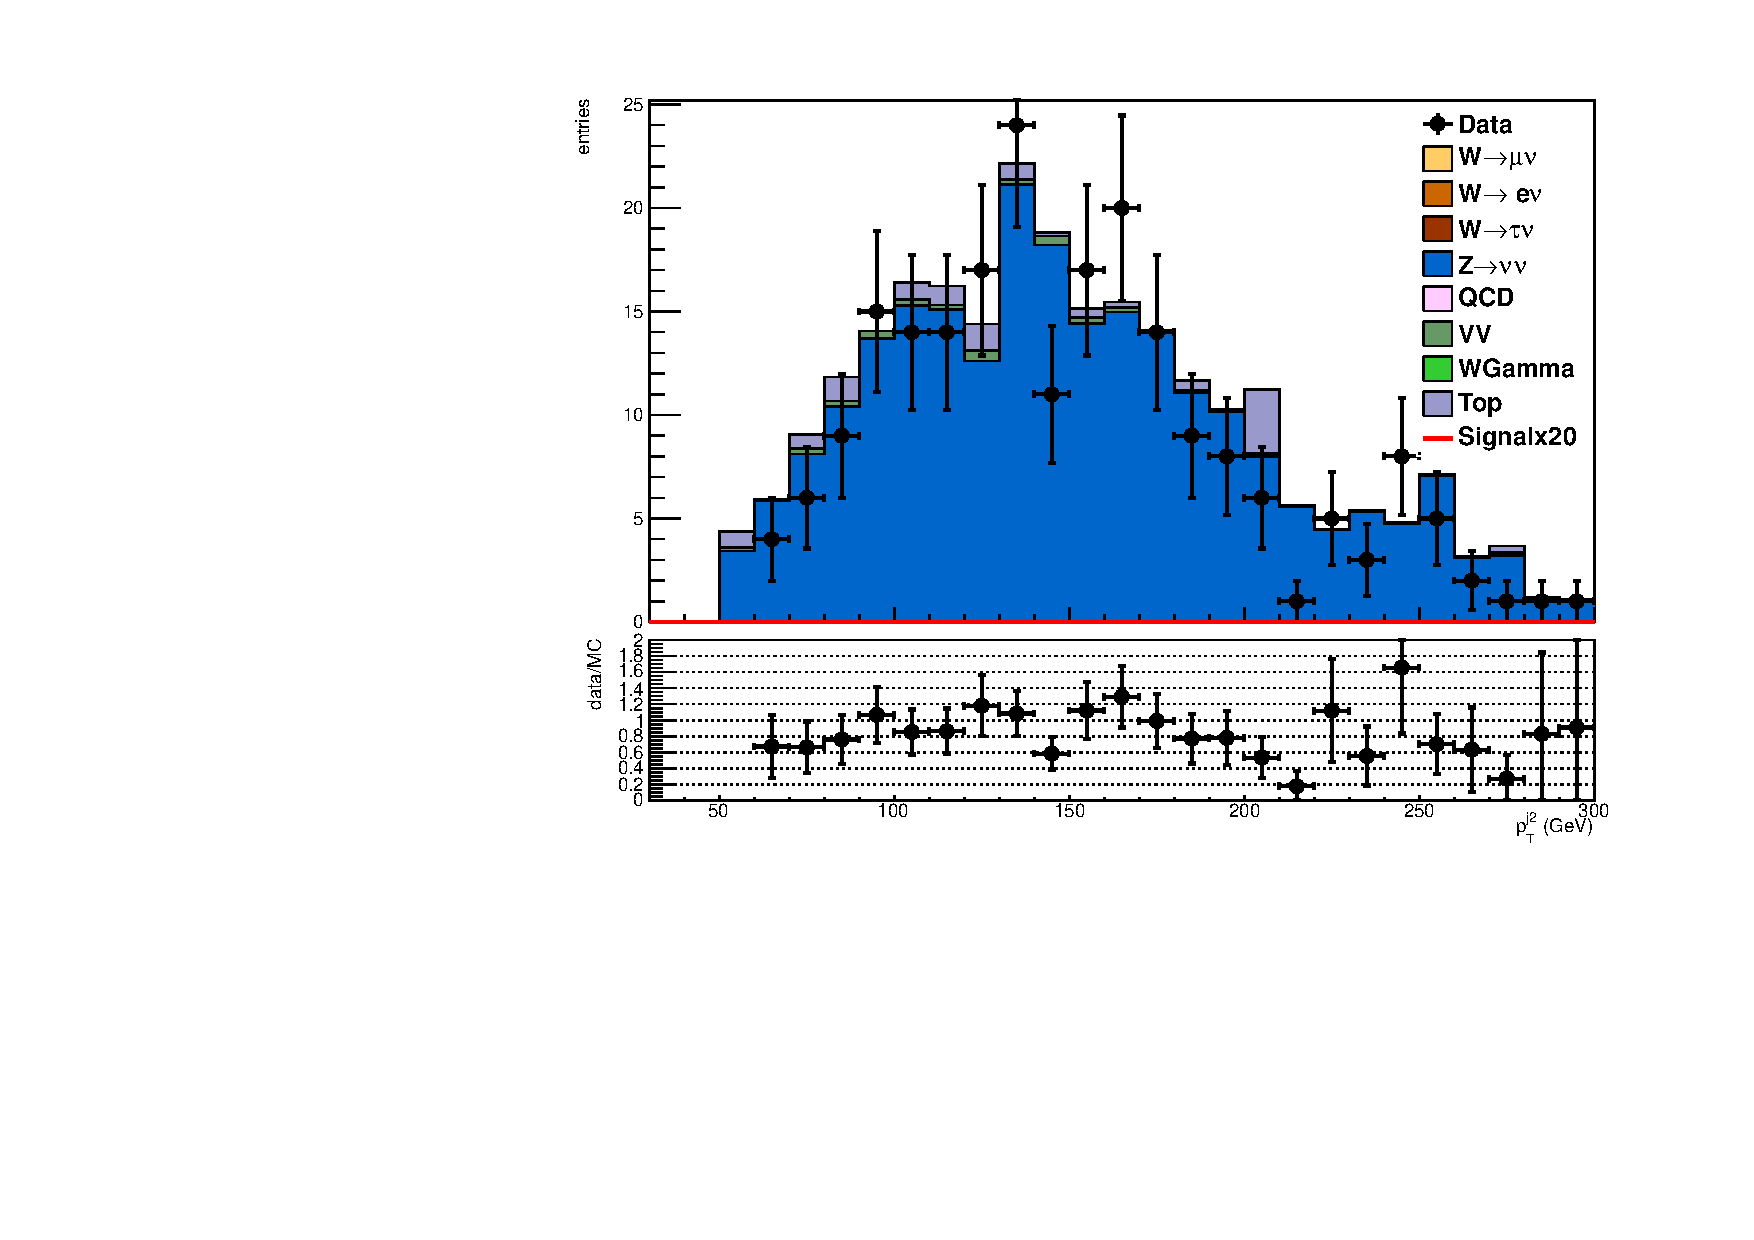
\includegraphics[width=\textwidth]{TalkPics/contplotsandpresel150914/output_contplots_alljetsmetdphicut10/mumu_jet1_pt.pdf}
    \end{block}
    \column{.5\textwidth}
    \begin{block}{Jet 2 pt}
      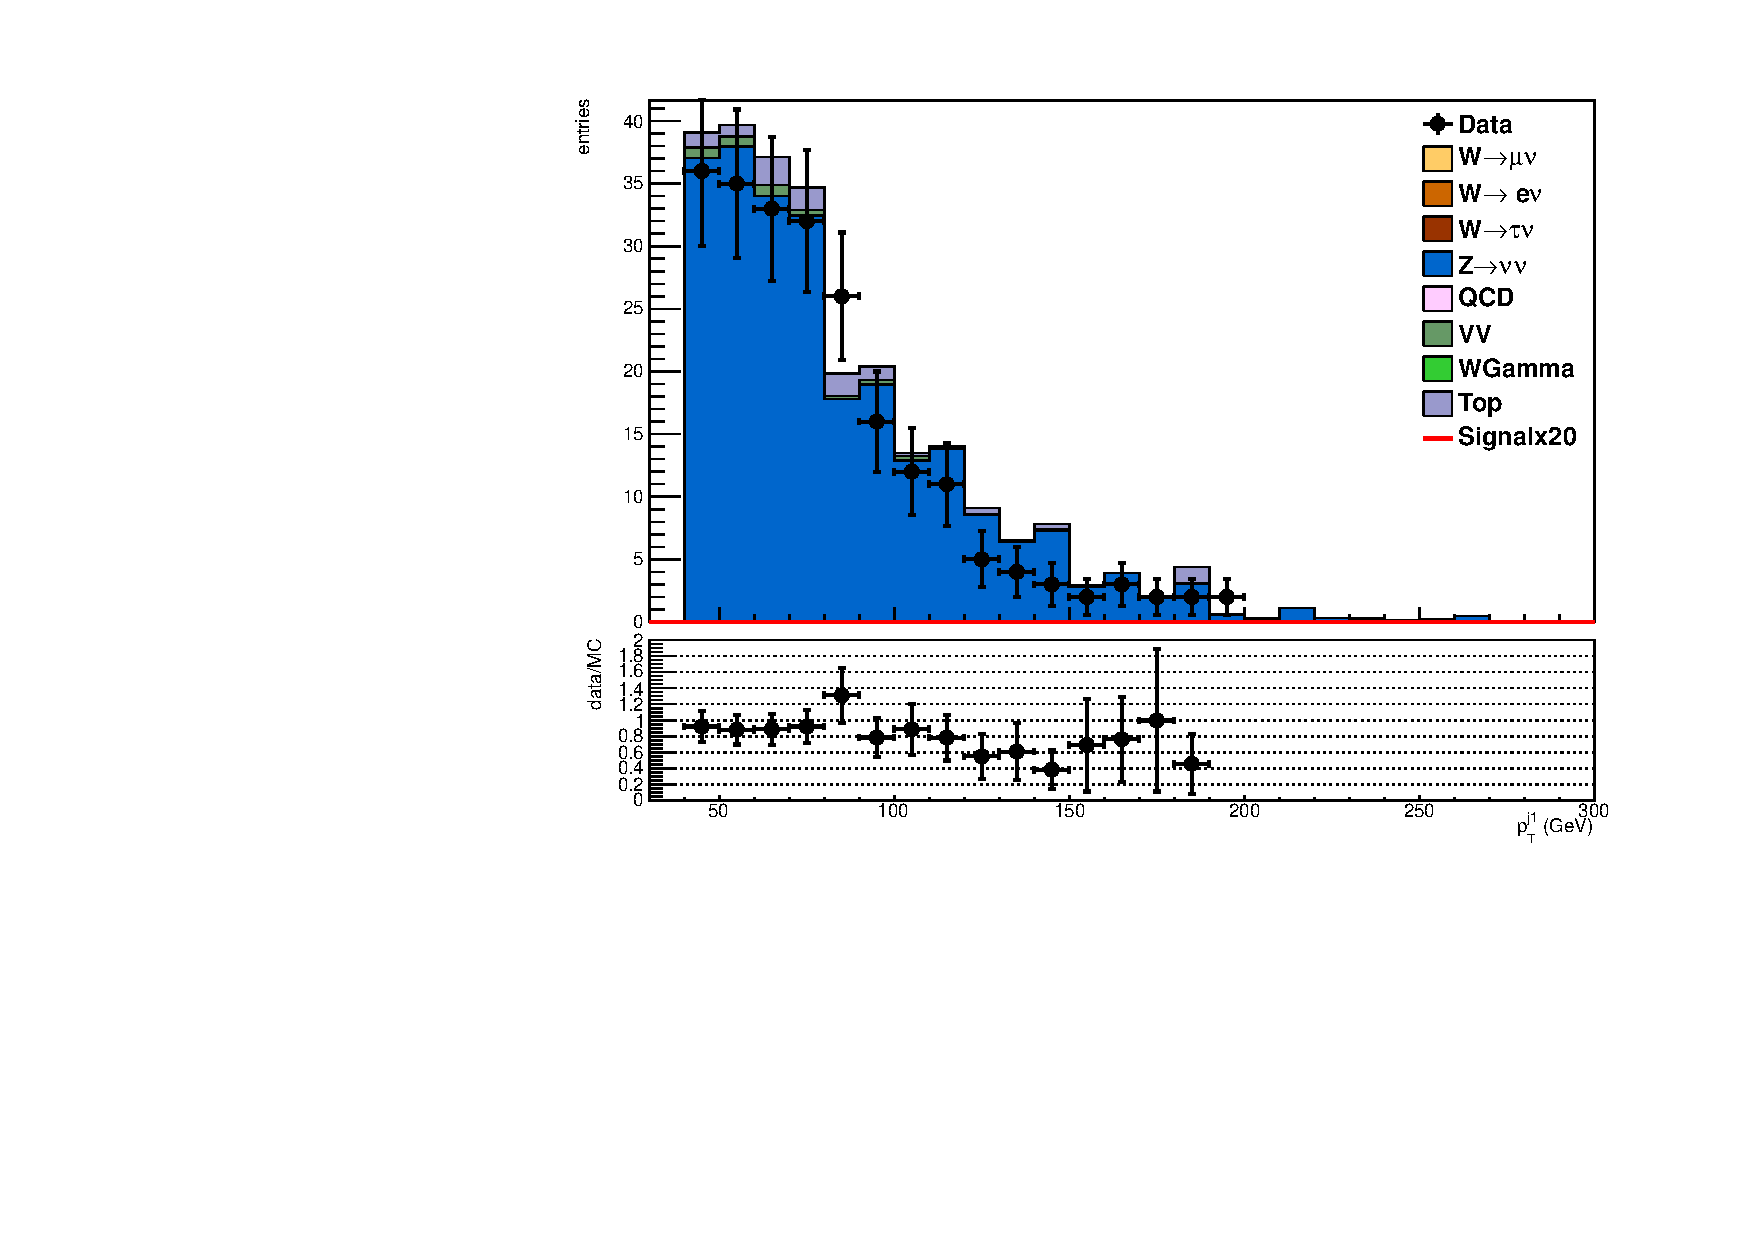
\includegraphics[width=\textwidth]{TalkPics/contplotsandpresel150914/output_contplots_alljetsmetdphicut10/mumu_jet2_pt.pdf}
    \end{block}

  \end{columns}
\end{frame}

\begin{frame}
  \frametitle{New control plots - mumu}
  \begin{columns}
    \column{.5\textwidth}
    \begin{block}{METnomu}
      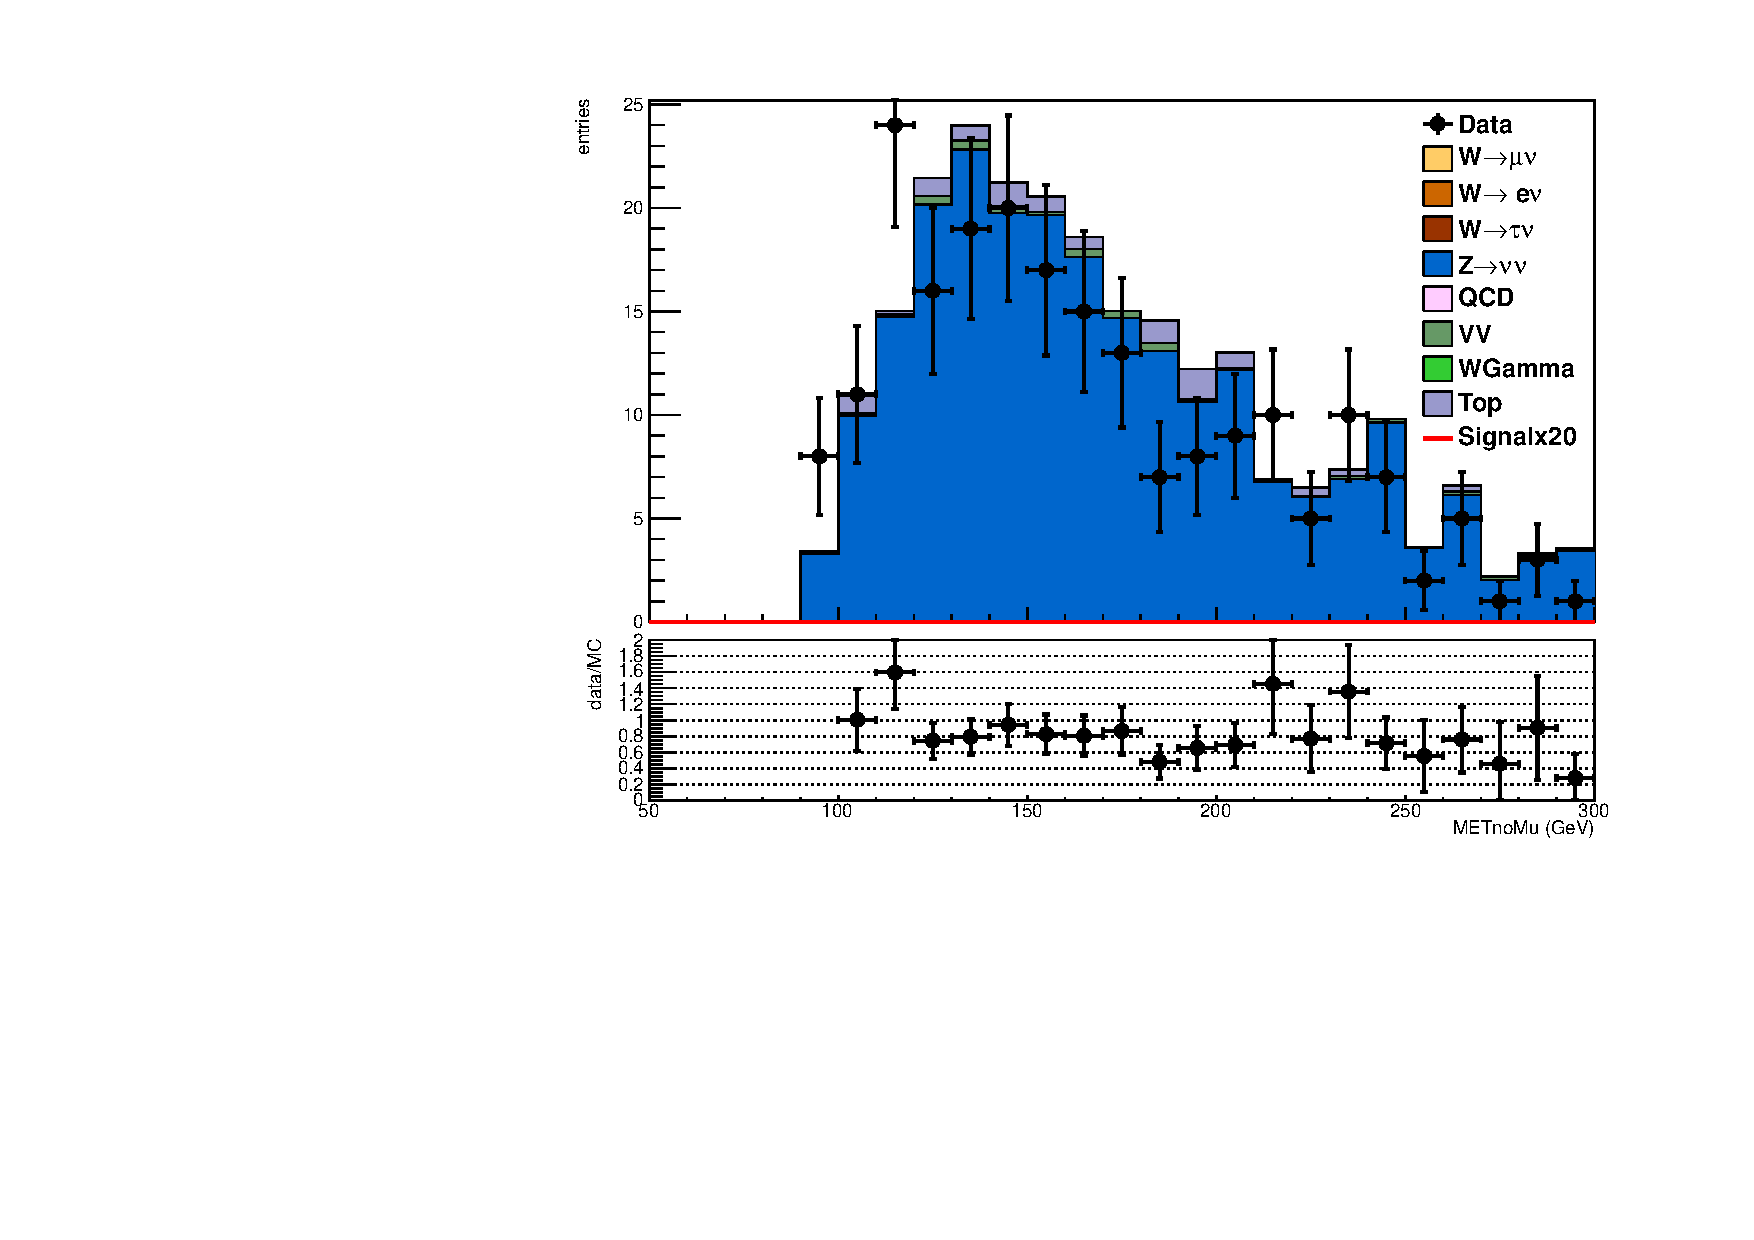
\includegraphics[width=\textwidth]{TalkPics/contplotsandpresel150914/output_contplots_alljetsmetdphicut10/mumu_metnomuons.pdf}
    \end{block}
    \column{.5\textwidth}
    \begin{block}{METnomusig}
      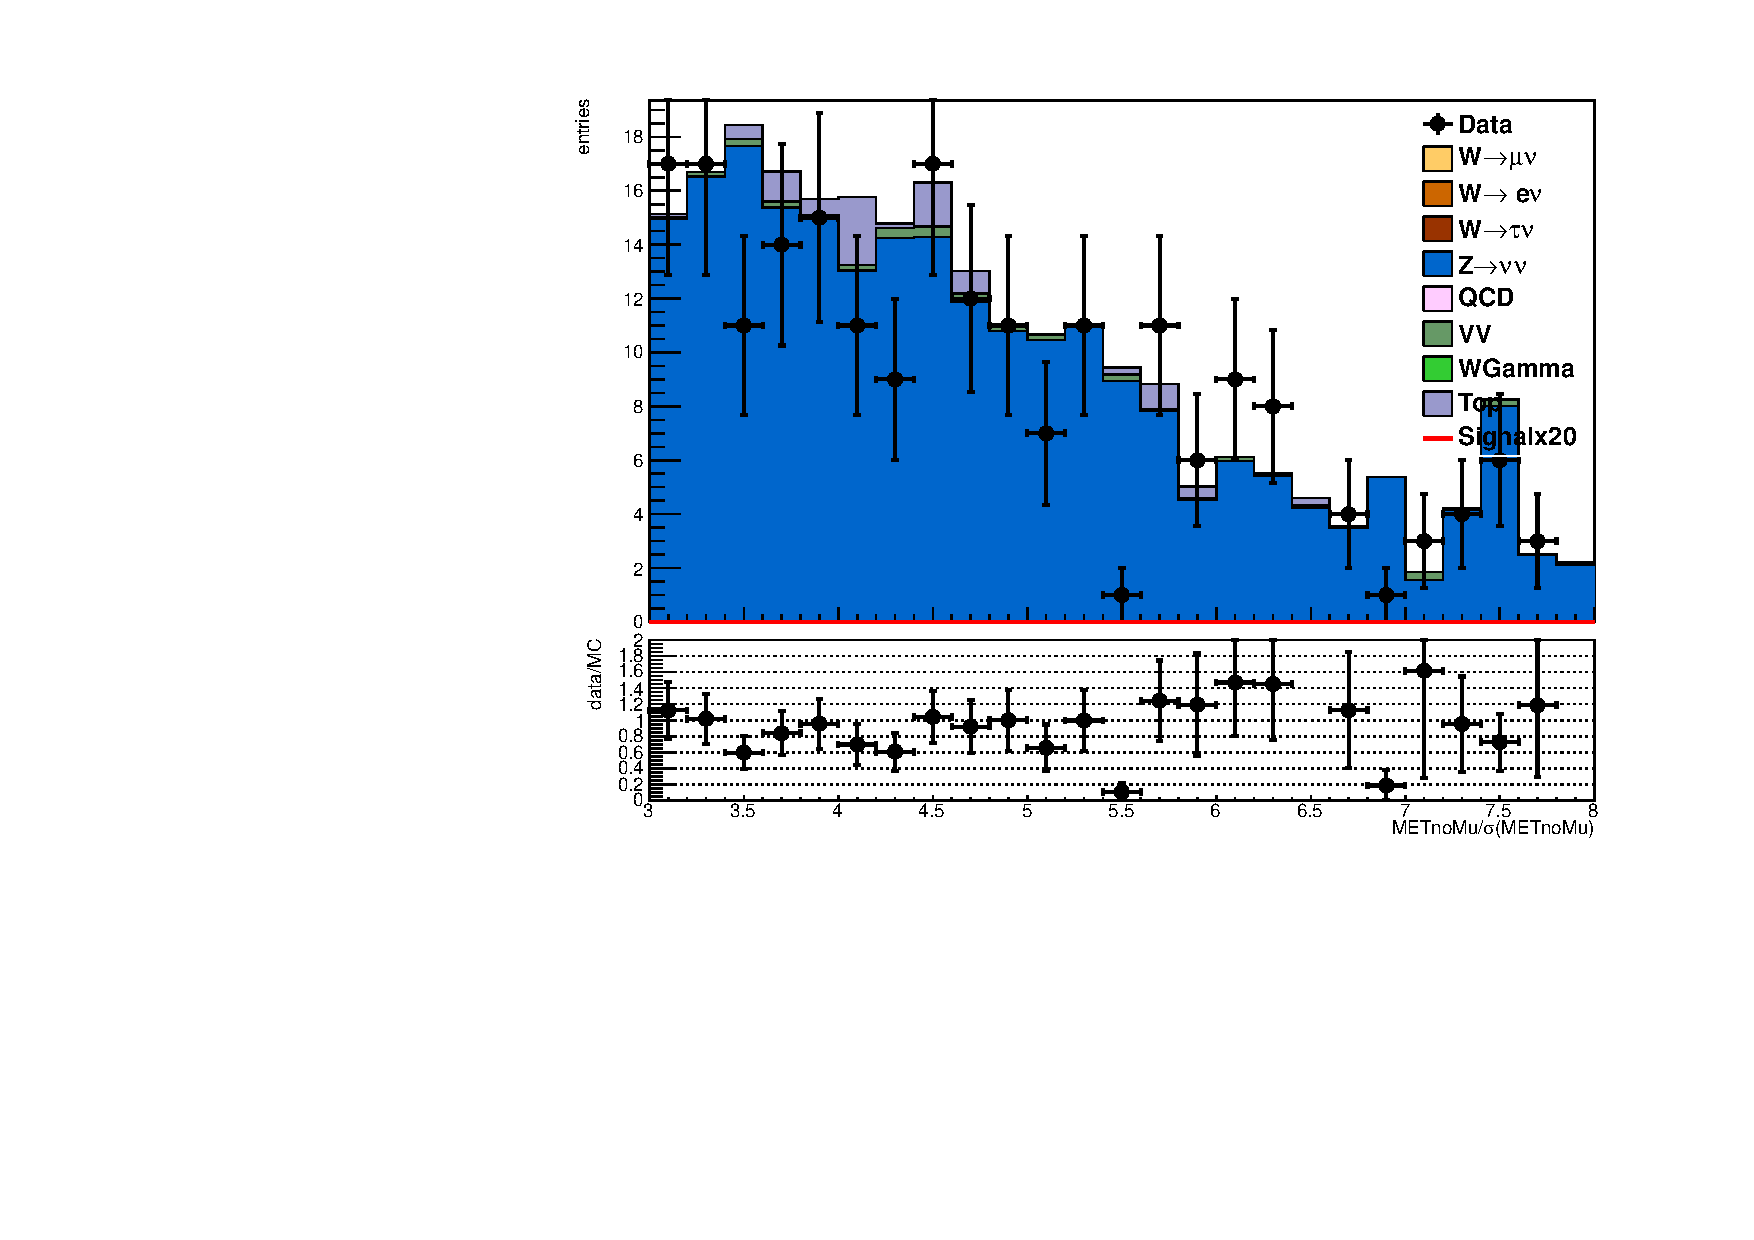
\includegraphics[width=\textwidth]{TalkPics/contplotsandpresel150914/output_contplots_alljetsmetdphicut10/mumu_metnomu_significance.pdf}
    \end{block}

  \end{columns}
\end{frame}

\begin{frame}
  \frametitle{New control plots - mumu }
  \begin{columns}
    \column{.5\textwidth}
    \begin{block}{Mjj}
      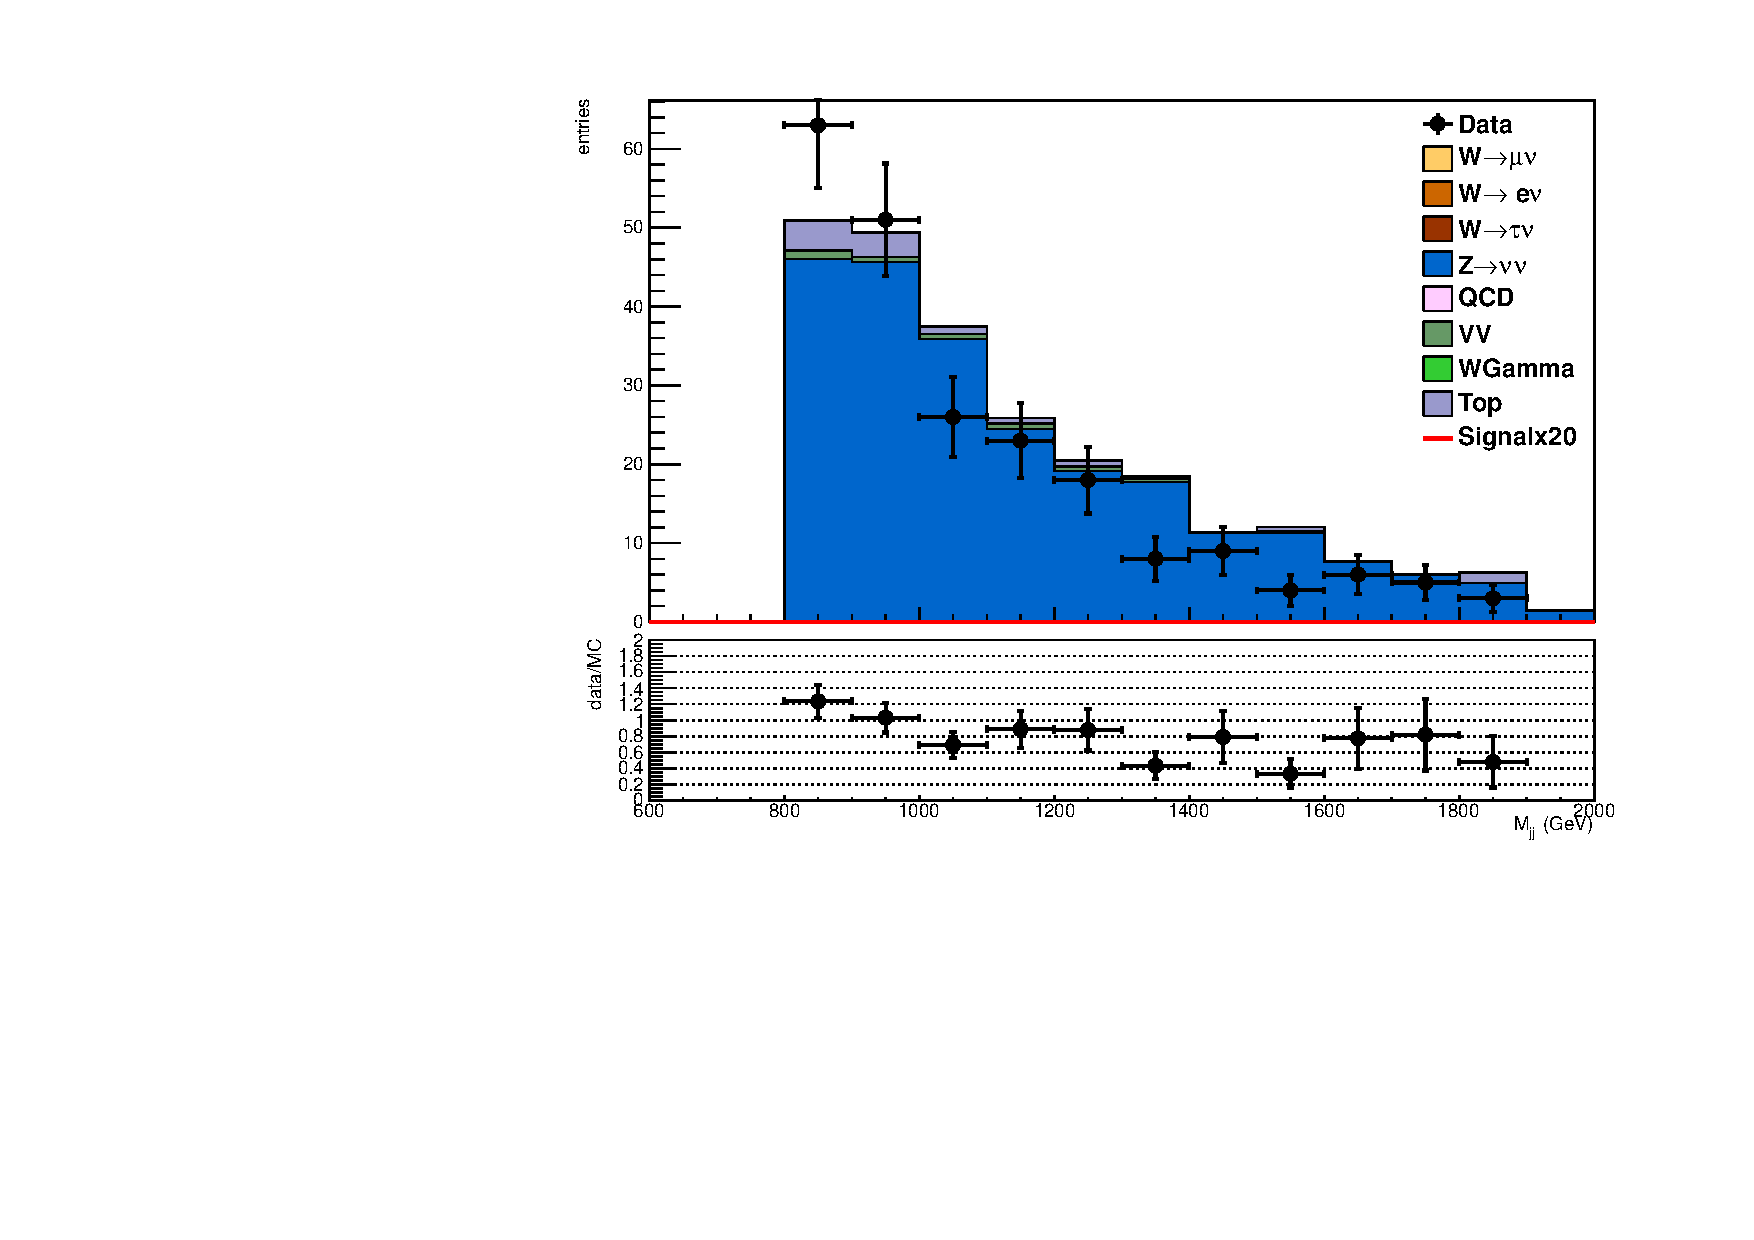
\includegraphics[width=\textwidth]{TalkPics/contplotsandpresel150914/output_contplots_alljetsmetdphicut10/mumu_dijet_M.pdf}
    \end{block}
    \column{.5\textwidth}
    \begin{block}{dijet-metnomu pt fraction}
      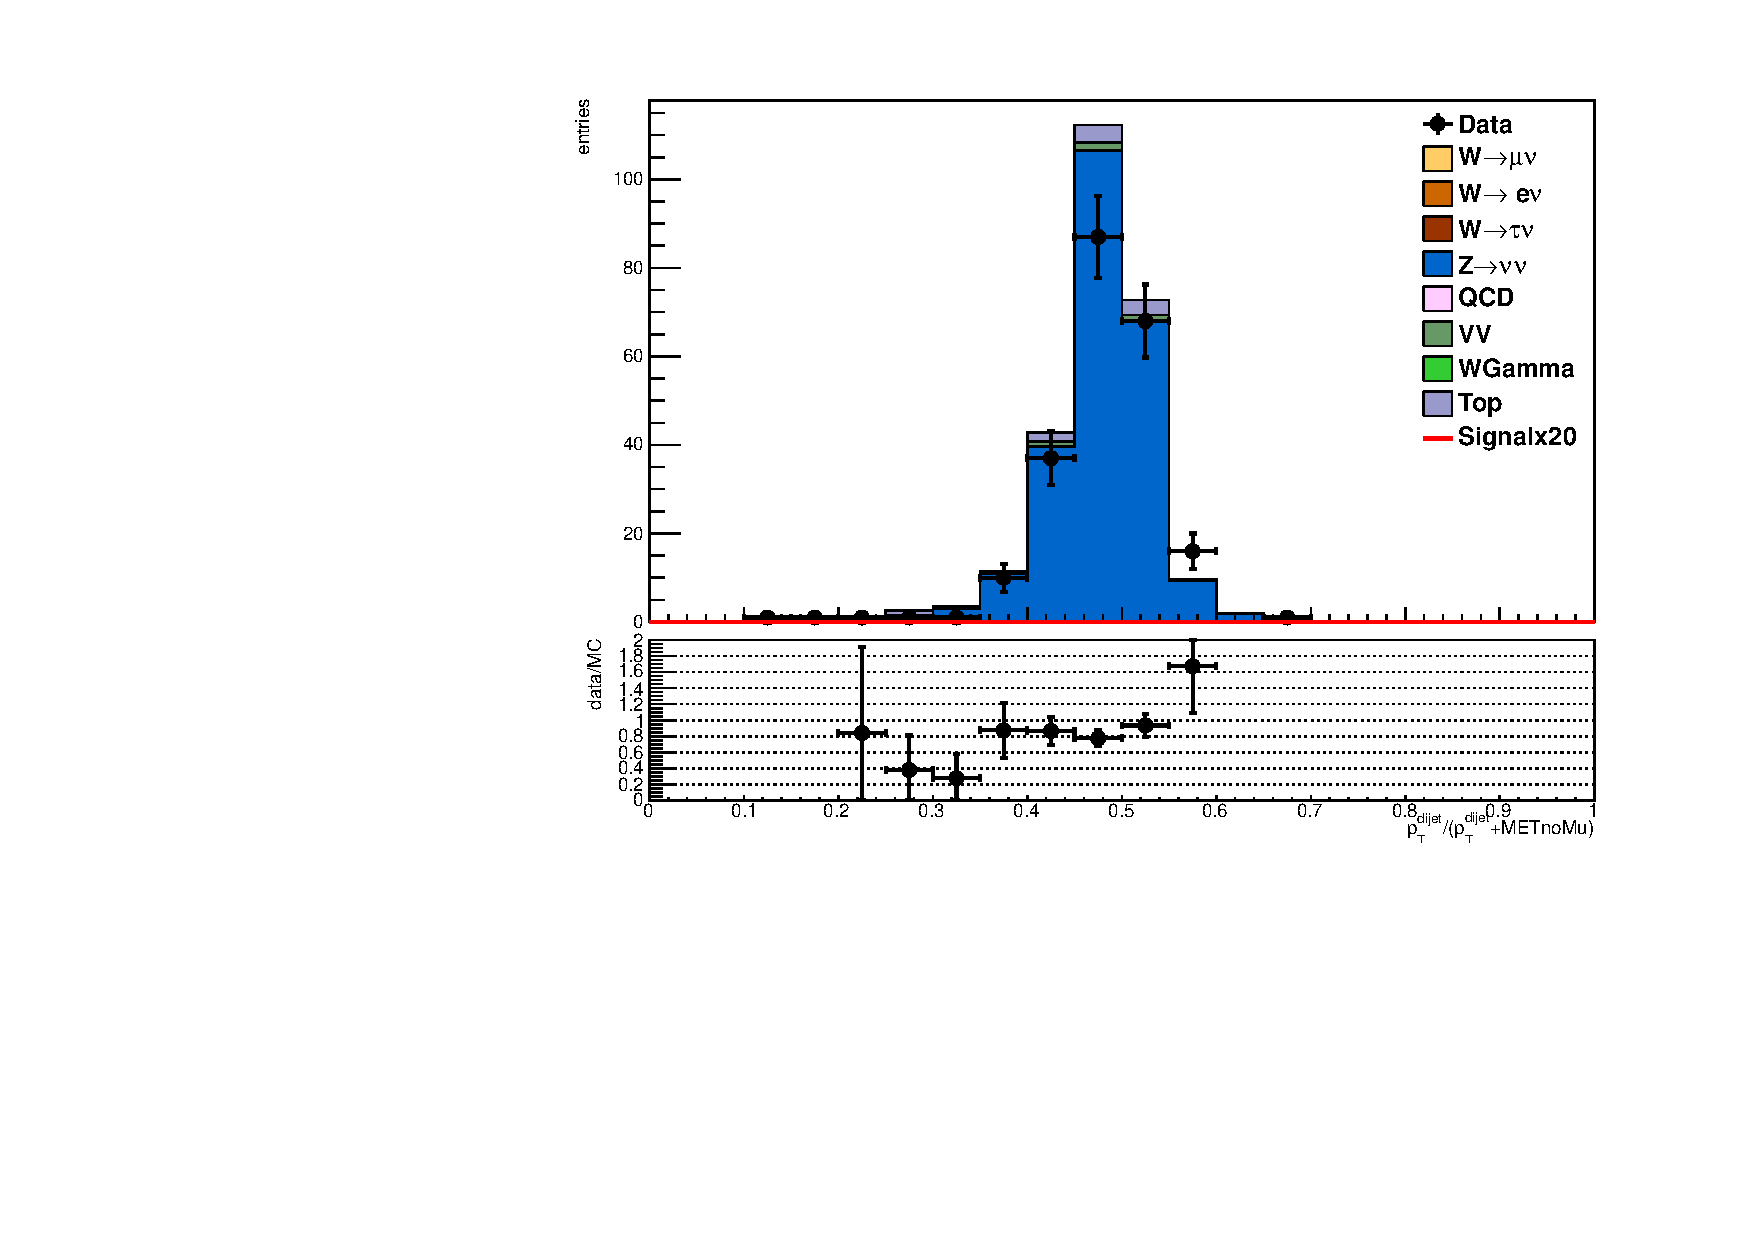
\includegraphics[width=\textwidth]{TalkPics/contplotsandpresel150914/output_contplots_alljetsmetdphicut10/mumu_dijetmetnomu_ptfraction.pdf}
    \end{block}
  \end{columns}
\end{frame}

\begin{frame}
  \frametitle{New control plots -mumu}
  \begin{columns}
    \column{.5\textwidth}
    \begin{block}{Dphijj}
      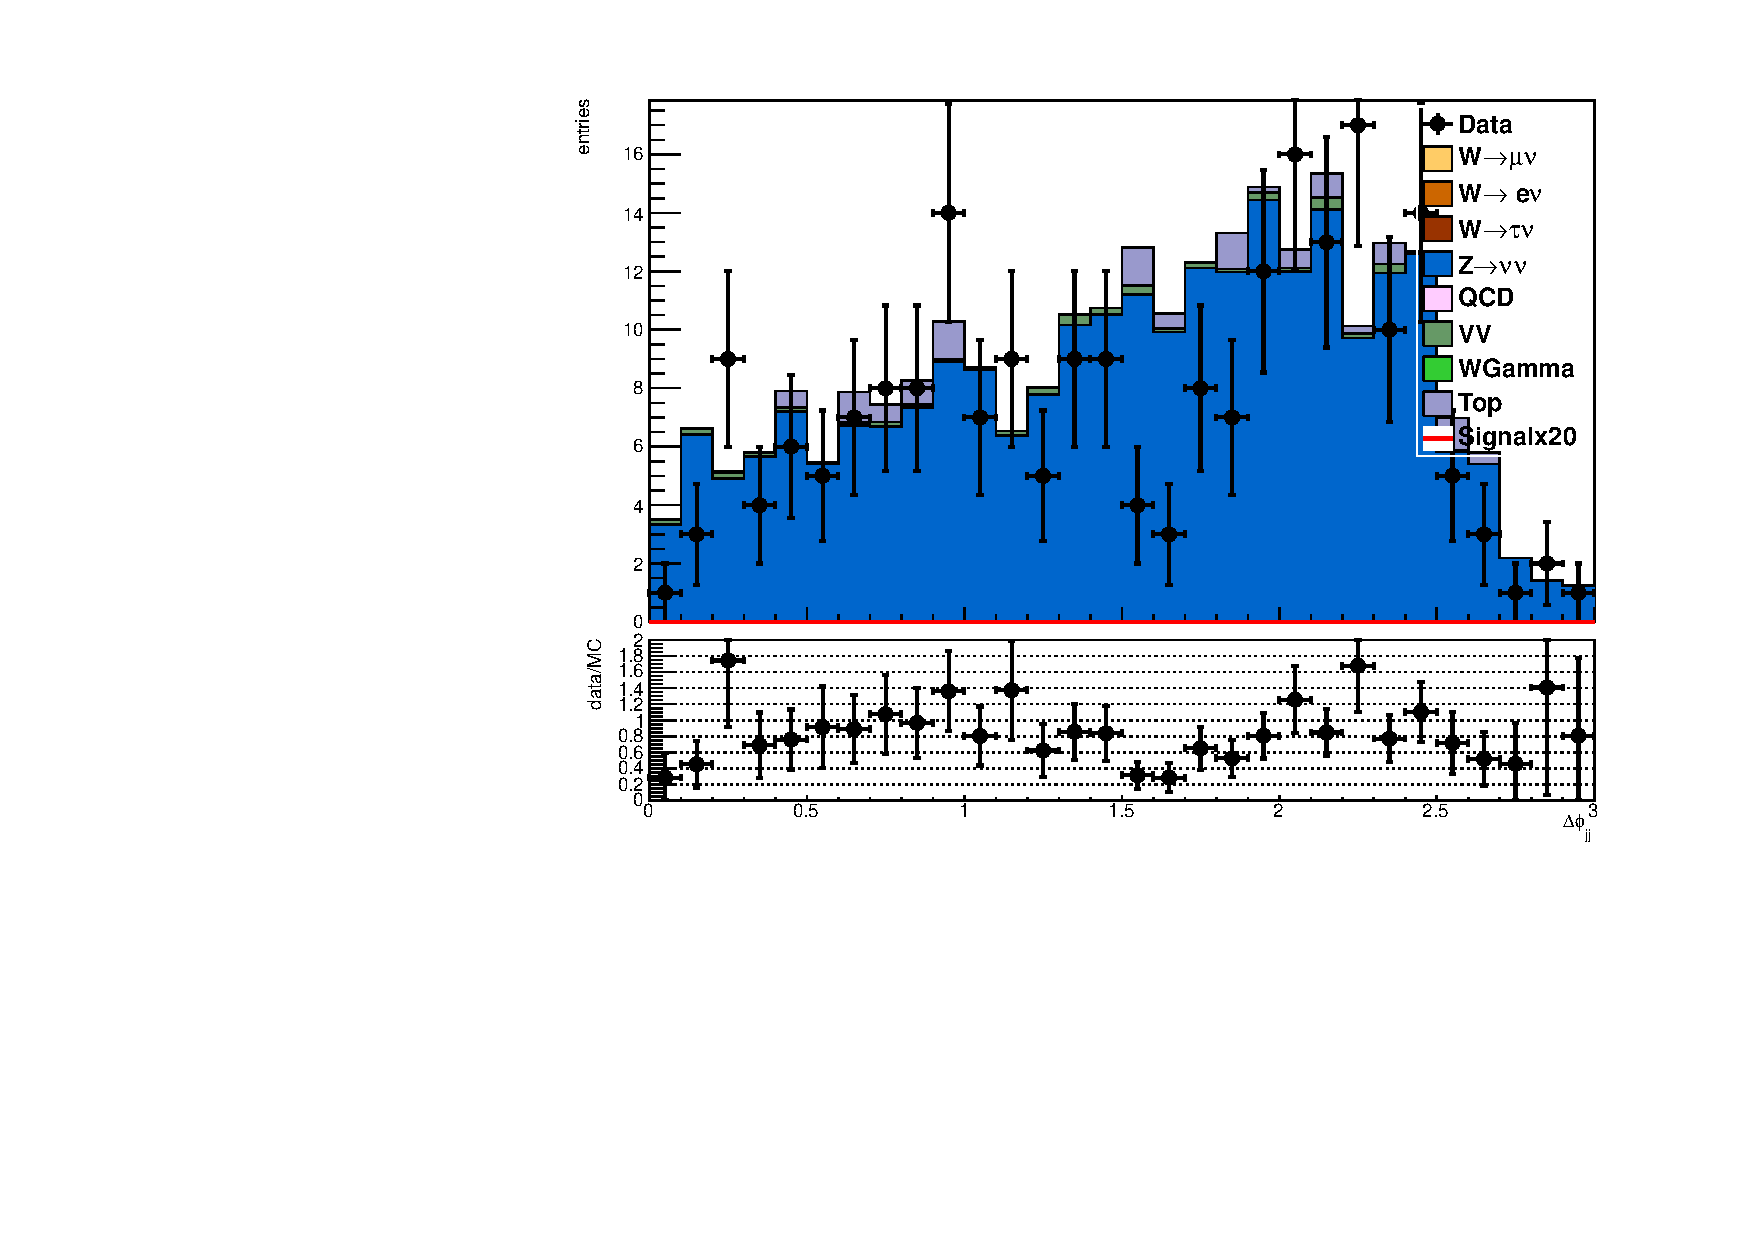
\includegraphics[width=\textwidth]{TalkPics/contplotsandpresel150914/output_contplots_alljetsmetdphicut10/mumu_dijet_dphi.pdf}
    \end{block}
    \column{.5\textwidth}
    \begin{block}{Detajj}
      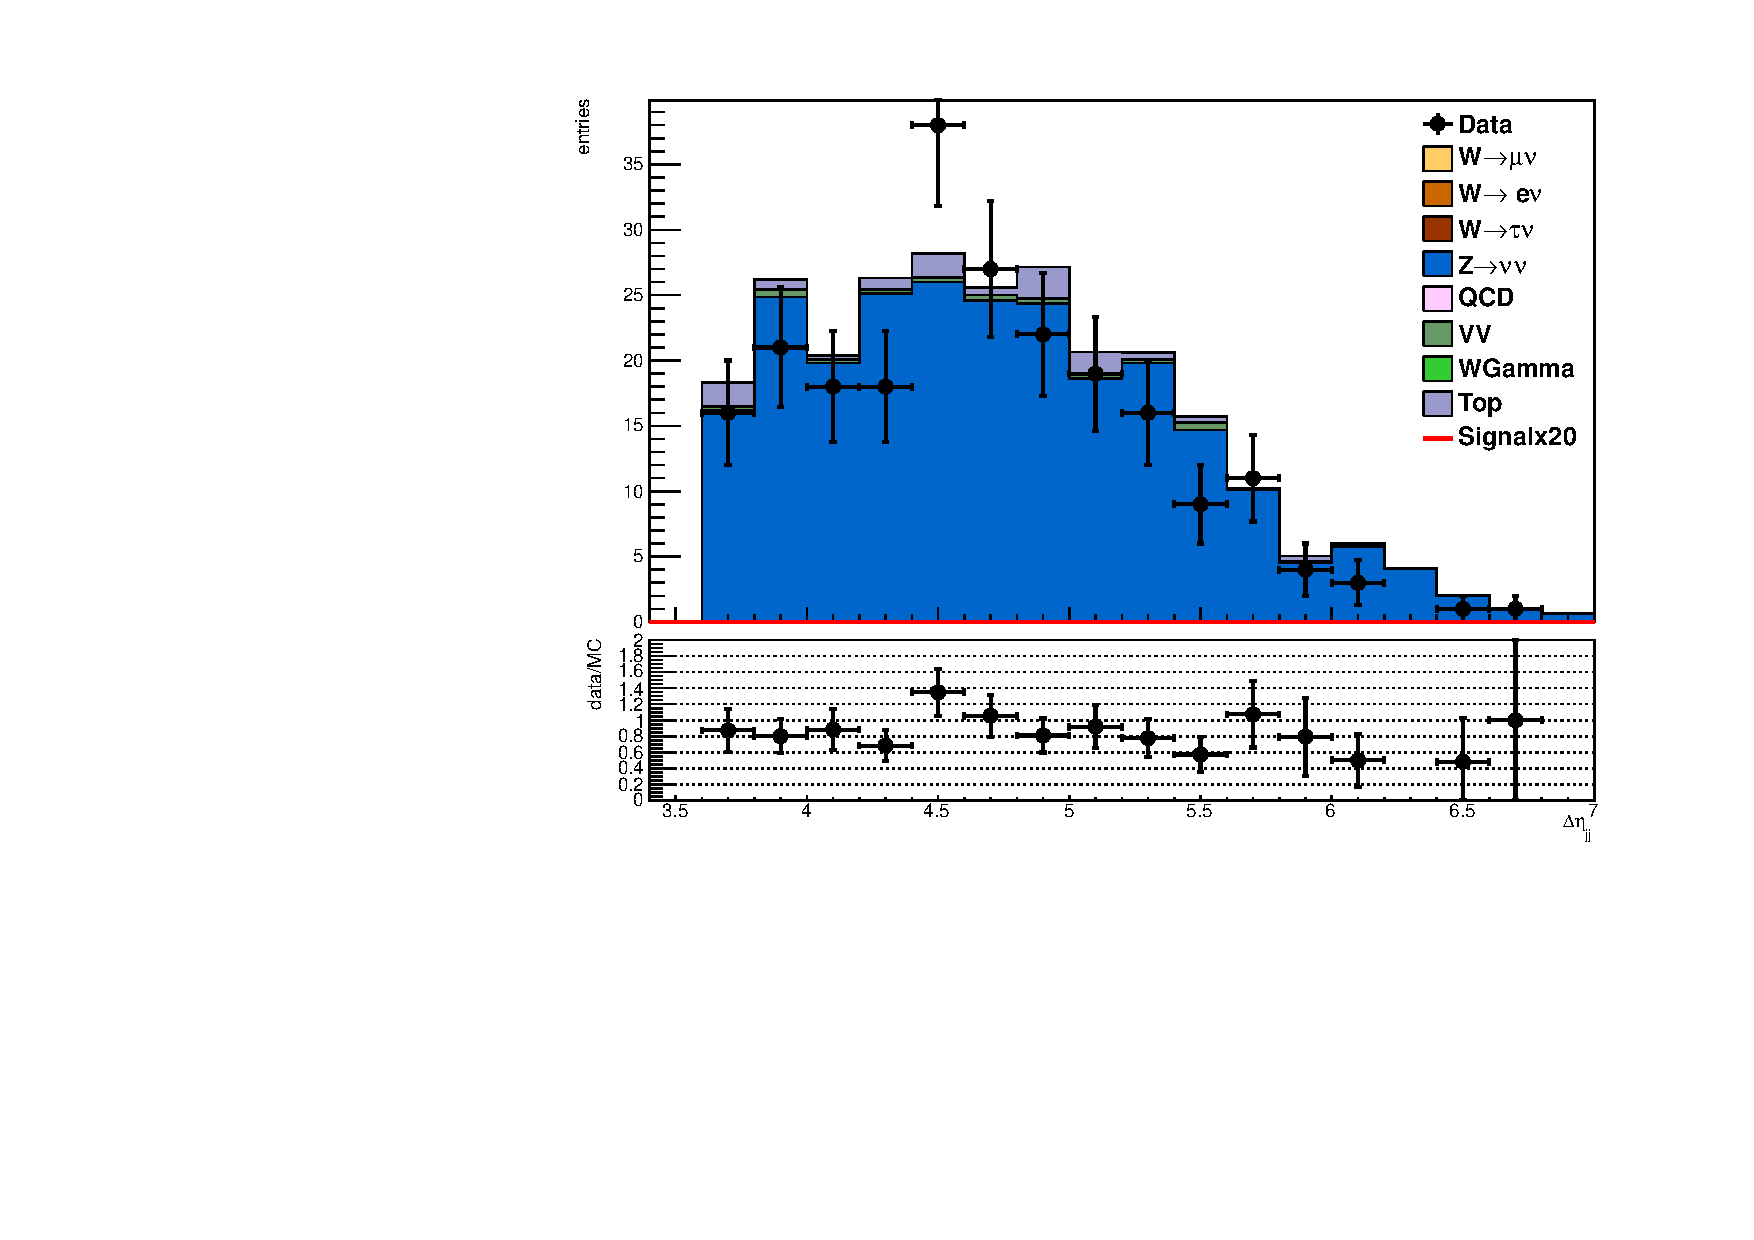
\includegraphics[width=\textwidth]{TalkPics/contplotsandpresel150914/output_contplots_alljetsmetdphicut10/mumu_dijet_deta.pdf}
    \end{block}

  \end{columns}
\end{frame}

\begin{frame}
  \frametitle{New control plots -mumu}
  \begin{columns}
    \column{.5\textwidth}
    \begin{block}{Leading jets-met mindphi}
      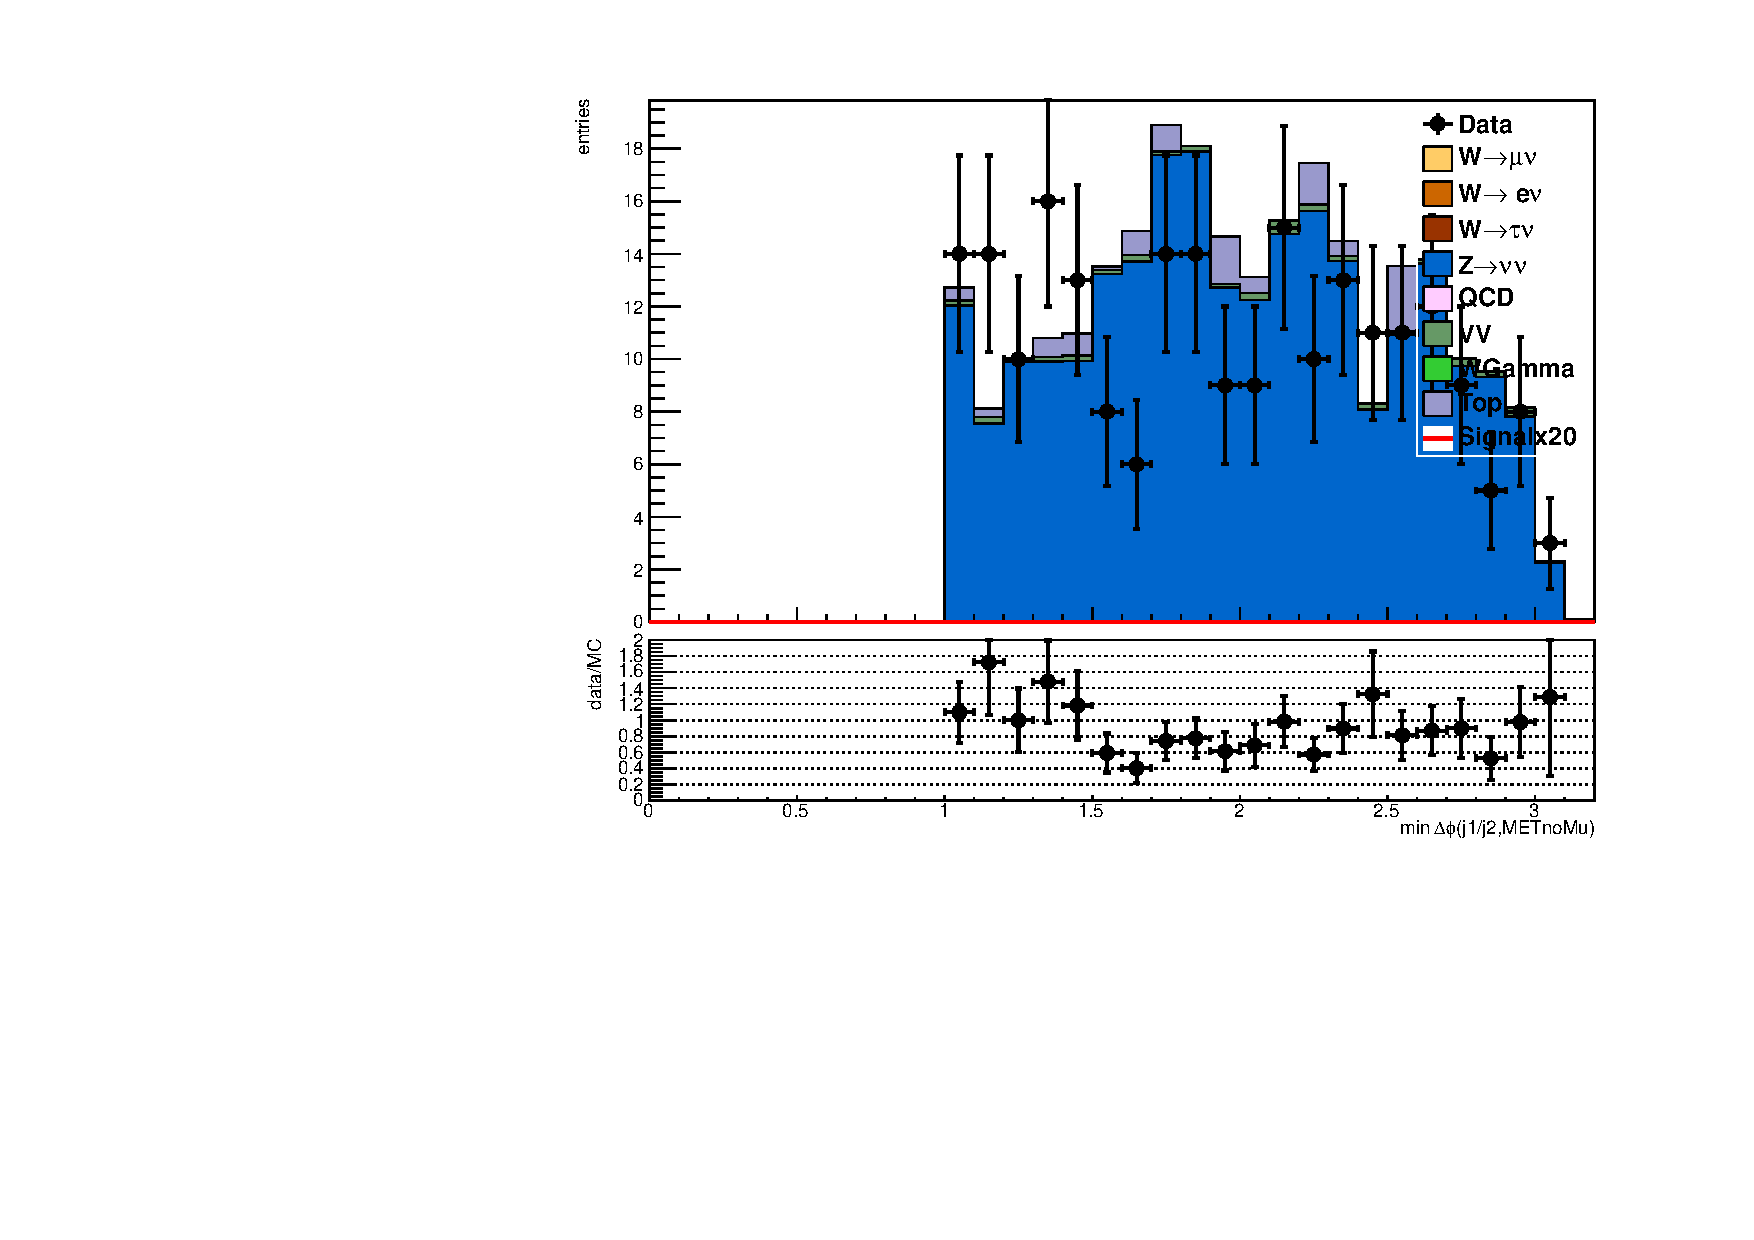
\includegraphics[width=\textwidth]{TalkPics/contplotsandpresel150914/output_contplots_alljetsmetdphicut10/mumu_jetmetnomu_mindphi.pdf}
    \end{block}
    \column{.5\textwidth}
    \begin{block}{All jet-met mindphi}
      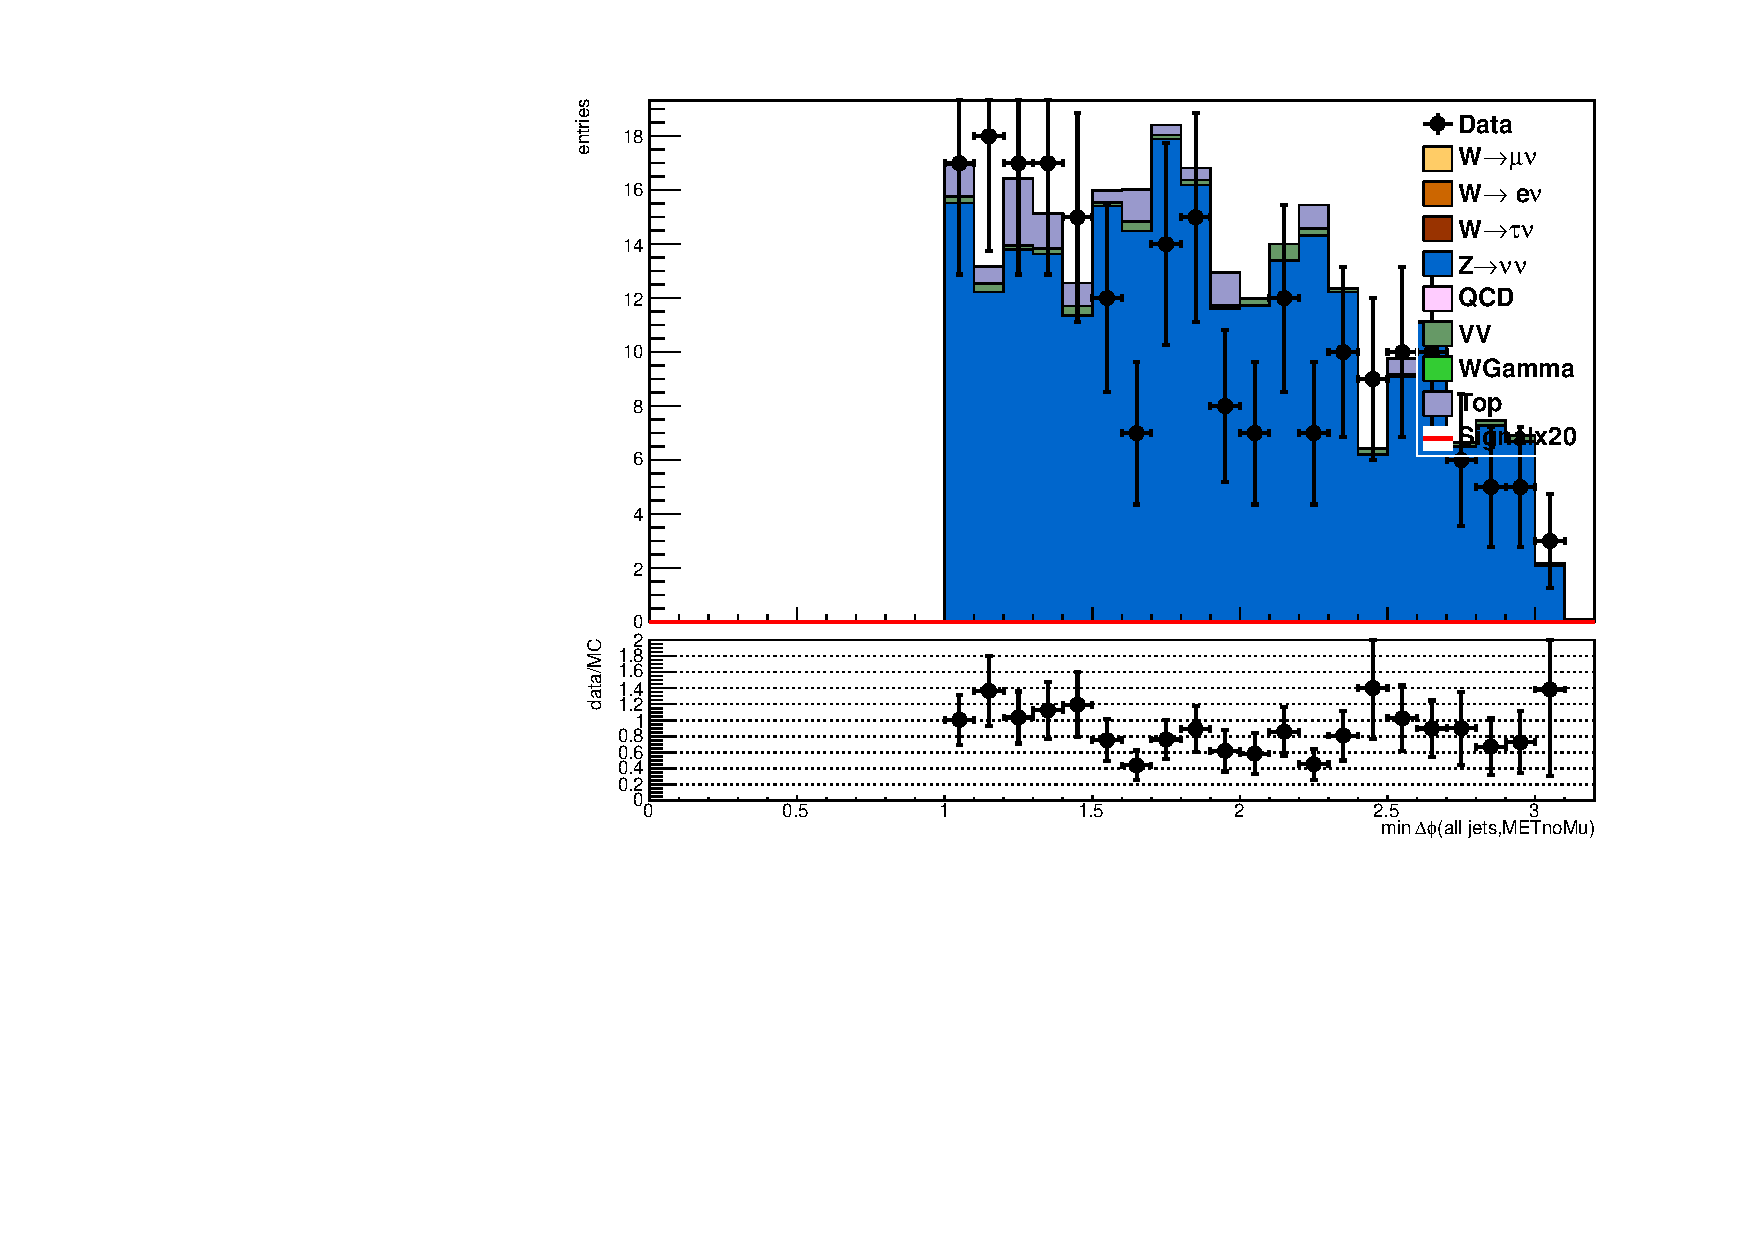
\includegraphics[width=\textwidth]{TalkPics/contplotsandpresel150914/output_contplots_alljetsmetdphicut10/mumu_alljetsmetnomu_mindphi.pdf}
    \end{block}

  \end{columns}
\end{frame}

\begin{frame}
  \frametitle{New control plots -enu}
  \begin{columns}
    \column{.5\textwidth}
    \begin{block}{Jet 1 pt}
      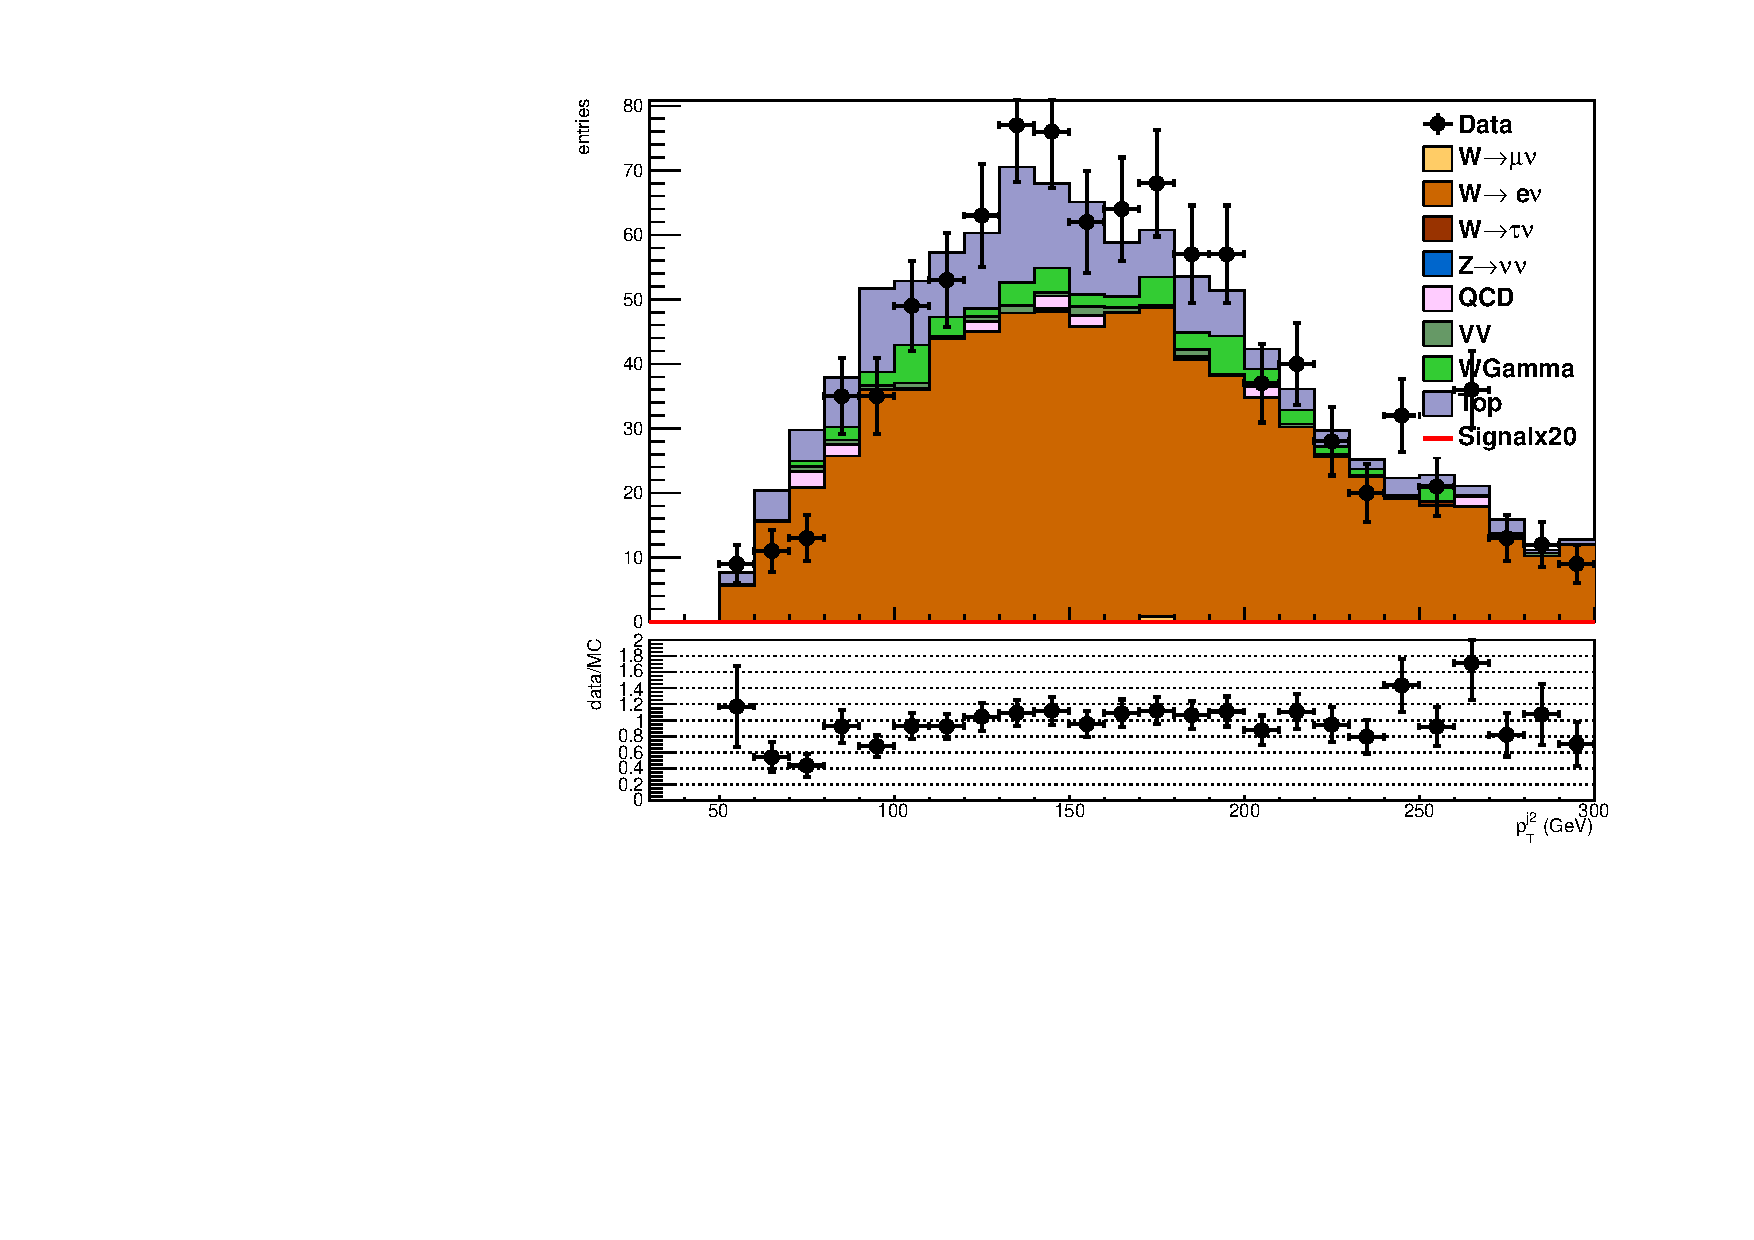
\includegraphics[width=\textwidth]{TalkPics/contplotsandpresel150914/output_contplots_alljetsmetdphicut10/enu_jet1_pt.pdf}
    \end{block}
    \column{.5\textwidth}
    \begin{block}{Jet 2 pt}
      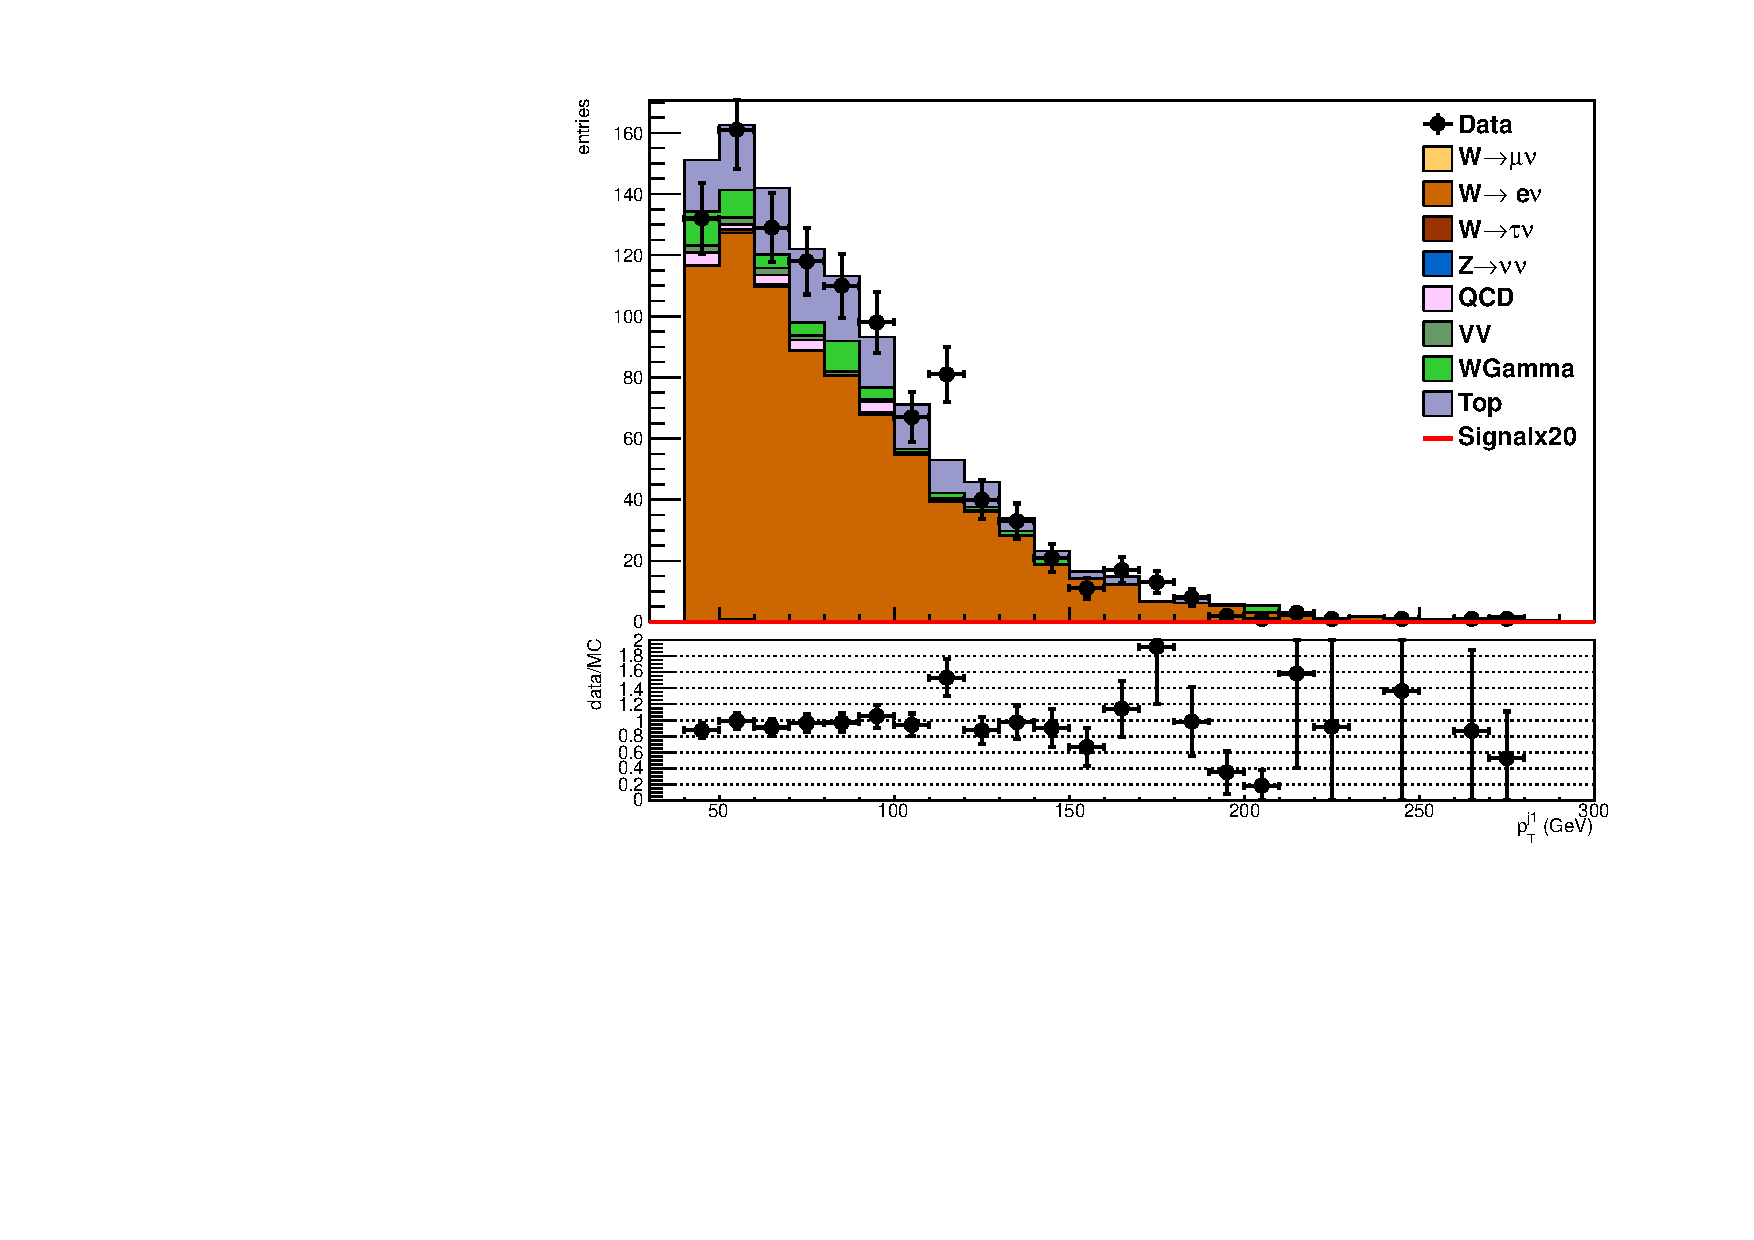
\includegraphics[width=\textwidth]{TalkPics/contplotsandpresel150914/output_contplots_alljetsmetdphicut10/enu_jet2_pt.pdf}
    \end{block}

  \end{columns}
\end{frame}

\begin{frame}
  \frametitle{New control plots -enu}
  \begin{columns}
    \column{.5\textwidth}
    \begin{block}{METnomu}
      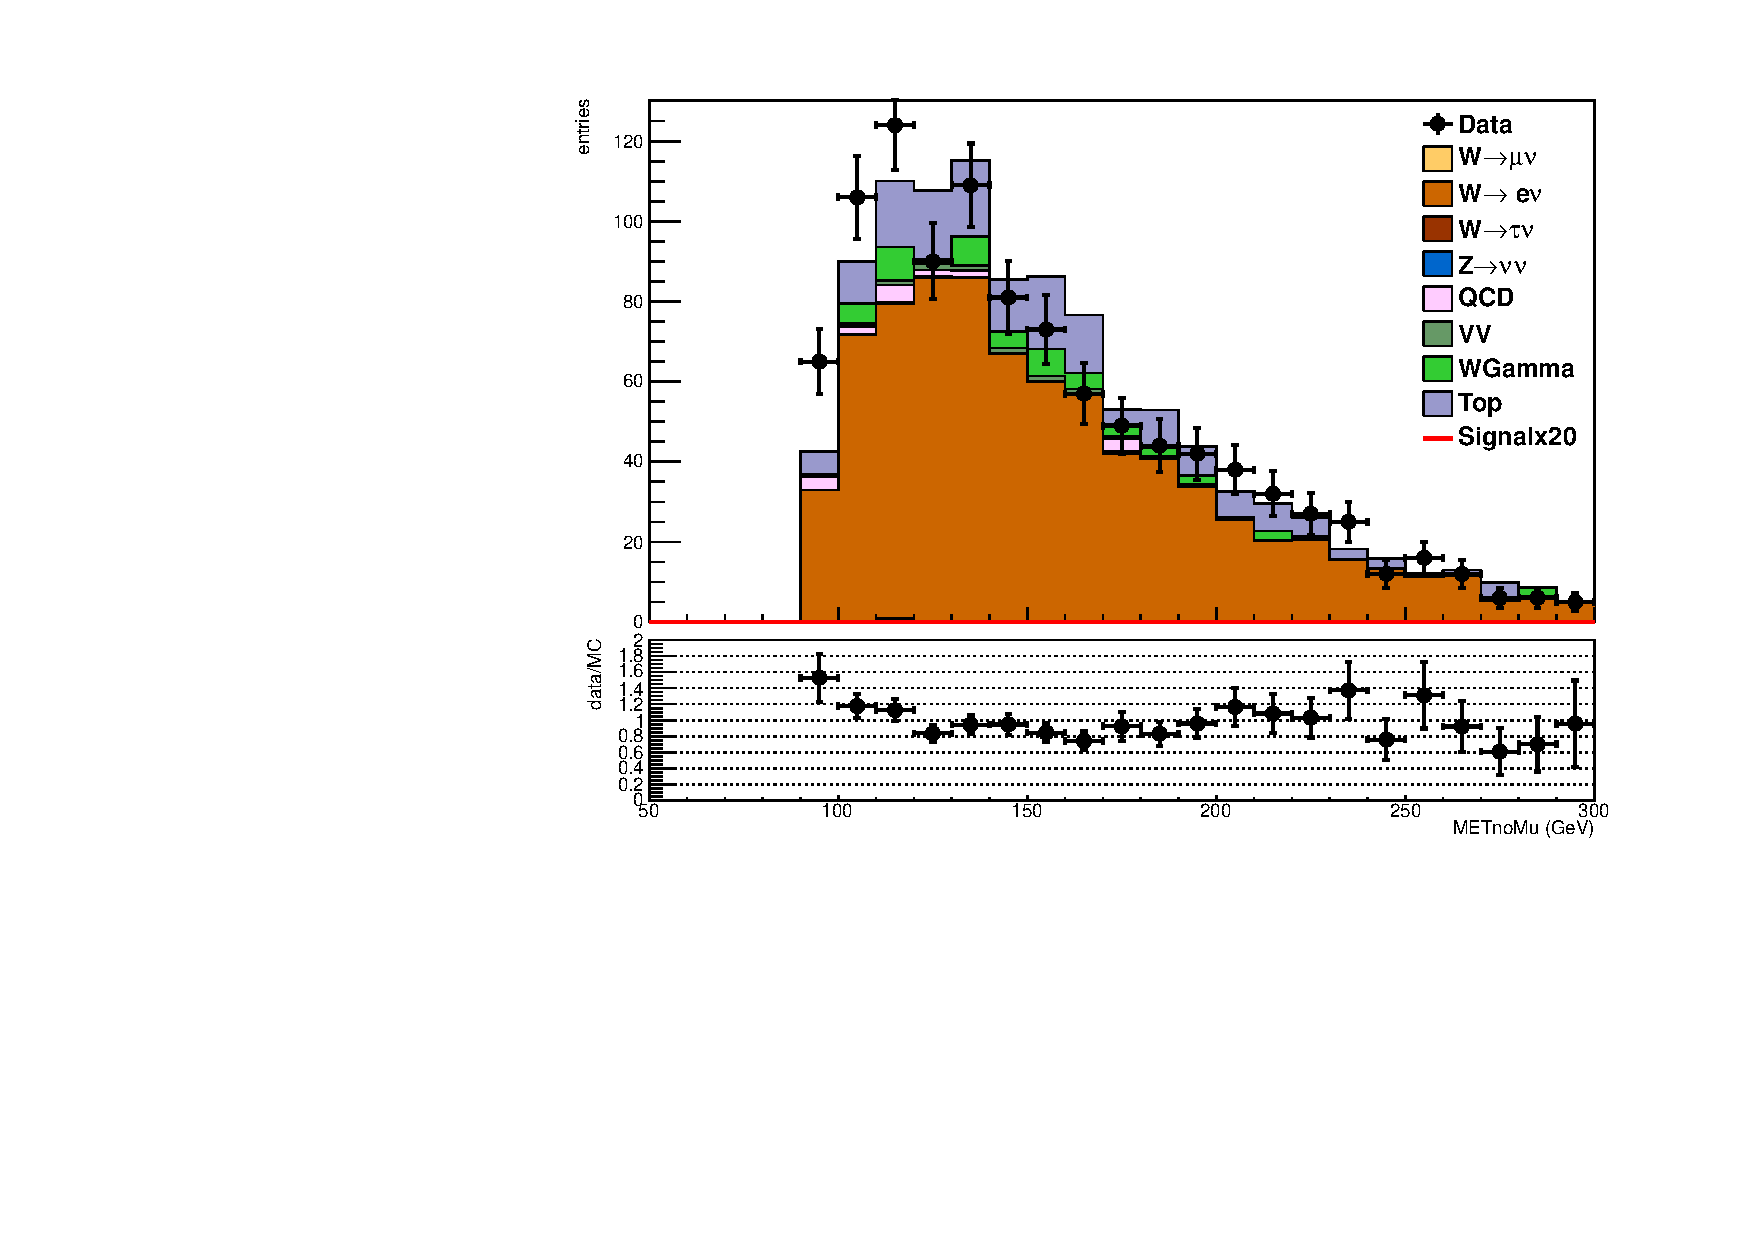
\includegraphics[width=\textwidth]{TalkPics/contplotsandpresel150914/output_contplots_alljetsmetdphicut10/enu_metnomuons.pdf}
    \end{block}
    \column{.5\textwidth}
    \begin{block}{METnomusig}
      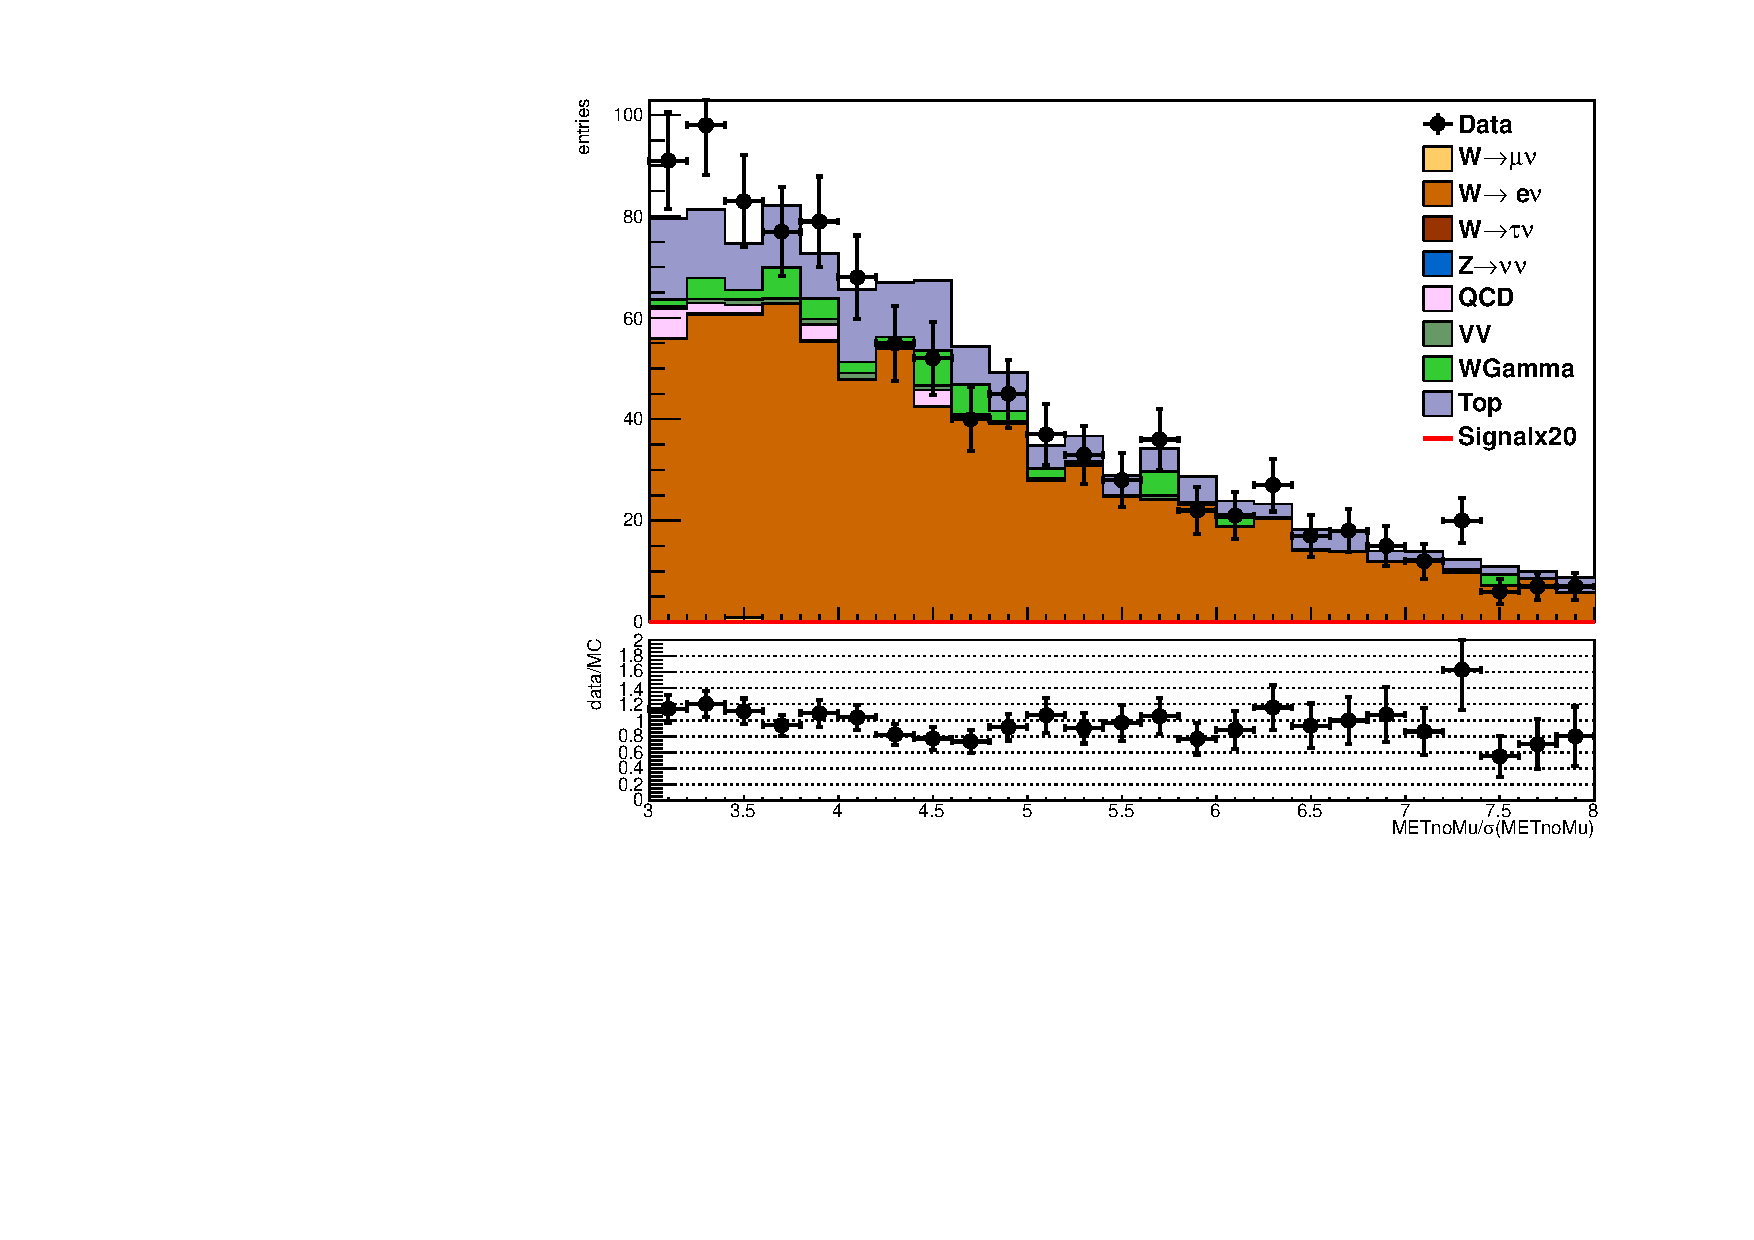
\includegraphics[width=\textwidth]{TalkPics/contplotsandpresel150914/output_contplots_alljetsmetdphicut10/enu_metnomu_significance.pdf}
    \end{block}

  \end{columns}
\end{frame}

\begin{frame}
  \frametitle{New control plots - enu}
  \begin{columns}
    \column{.5\textwidth}
    \begin{block}{Mjj}
      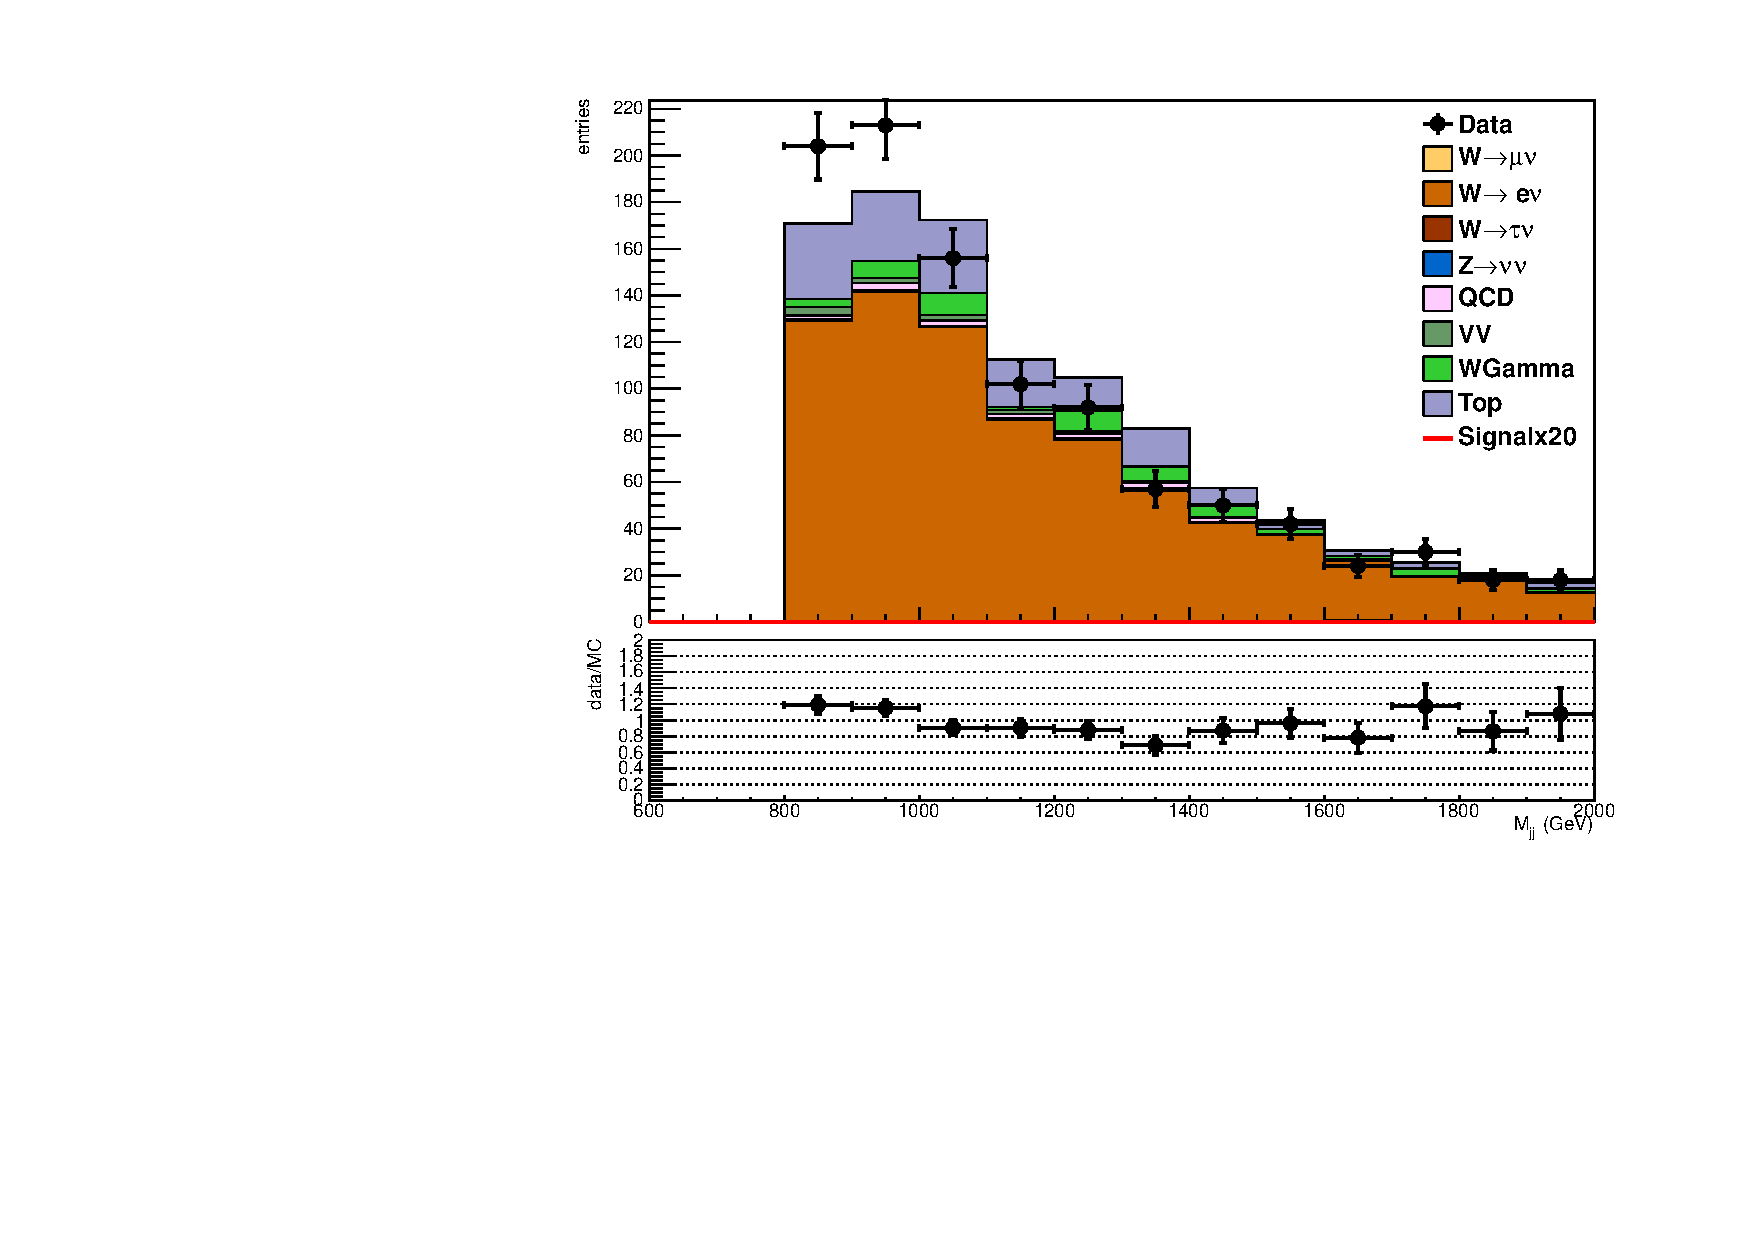
\includegraphics[width=\textwidth]{TalkPics/contplotsandpresel150914/output_contplots_alljetsmetdphicut10/enu_dijet_M.pdf}
    \end{block}
    \column{.5\textwidth}
    \begin{block}{mt}
      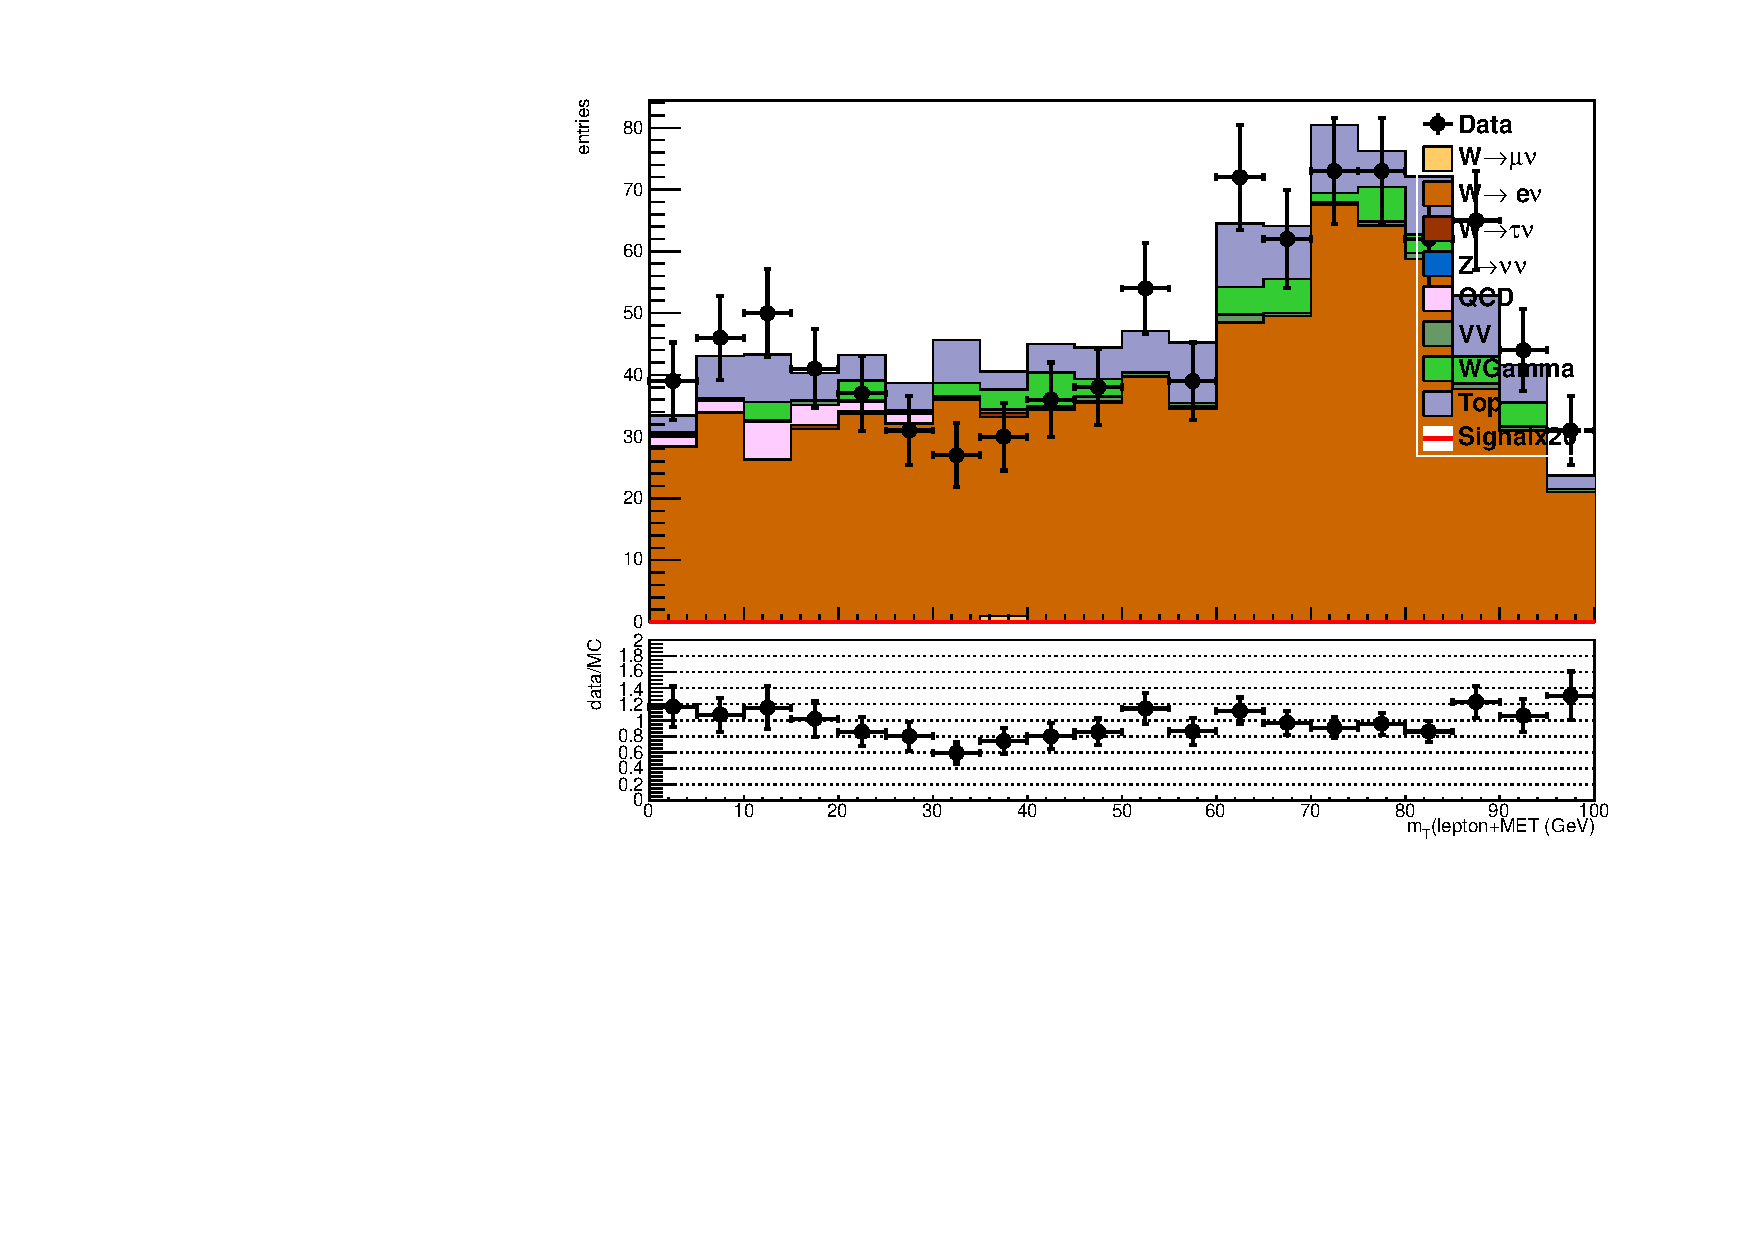
\includegraphics[width=\textwidth]{TalkPics/contplotsandpresel150914/output_contplots_alljetsmetdphicut10/enu_lep_mt.pdf}
    \end{block}
  \end{columns}
\end{frame}

\begin{frame}
  \frametitle{New control plots - enu}
  \begin{columns}
    \column{.5\textwidth}
    \begin{block}{Dijet Dphi}
      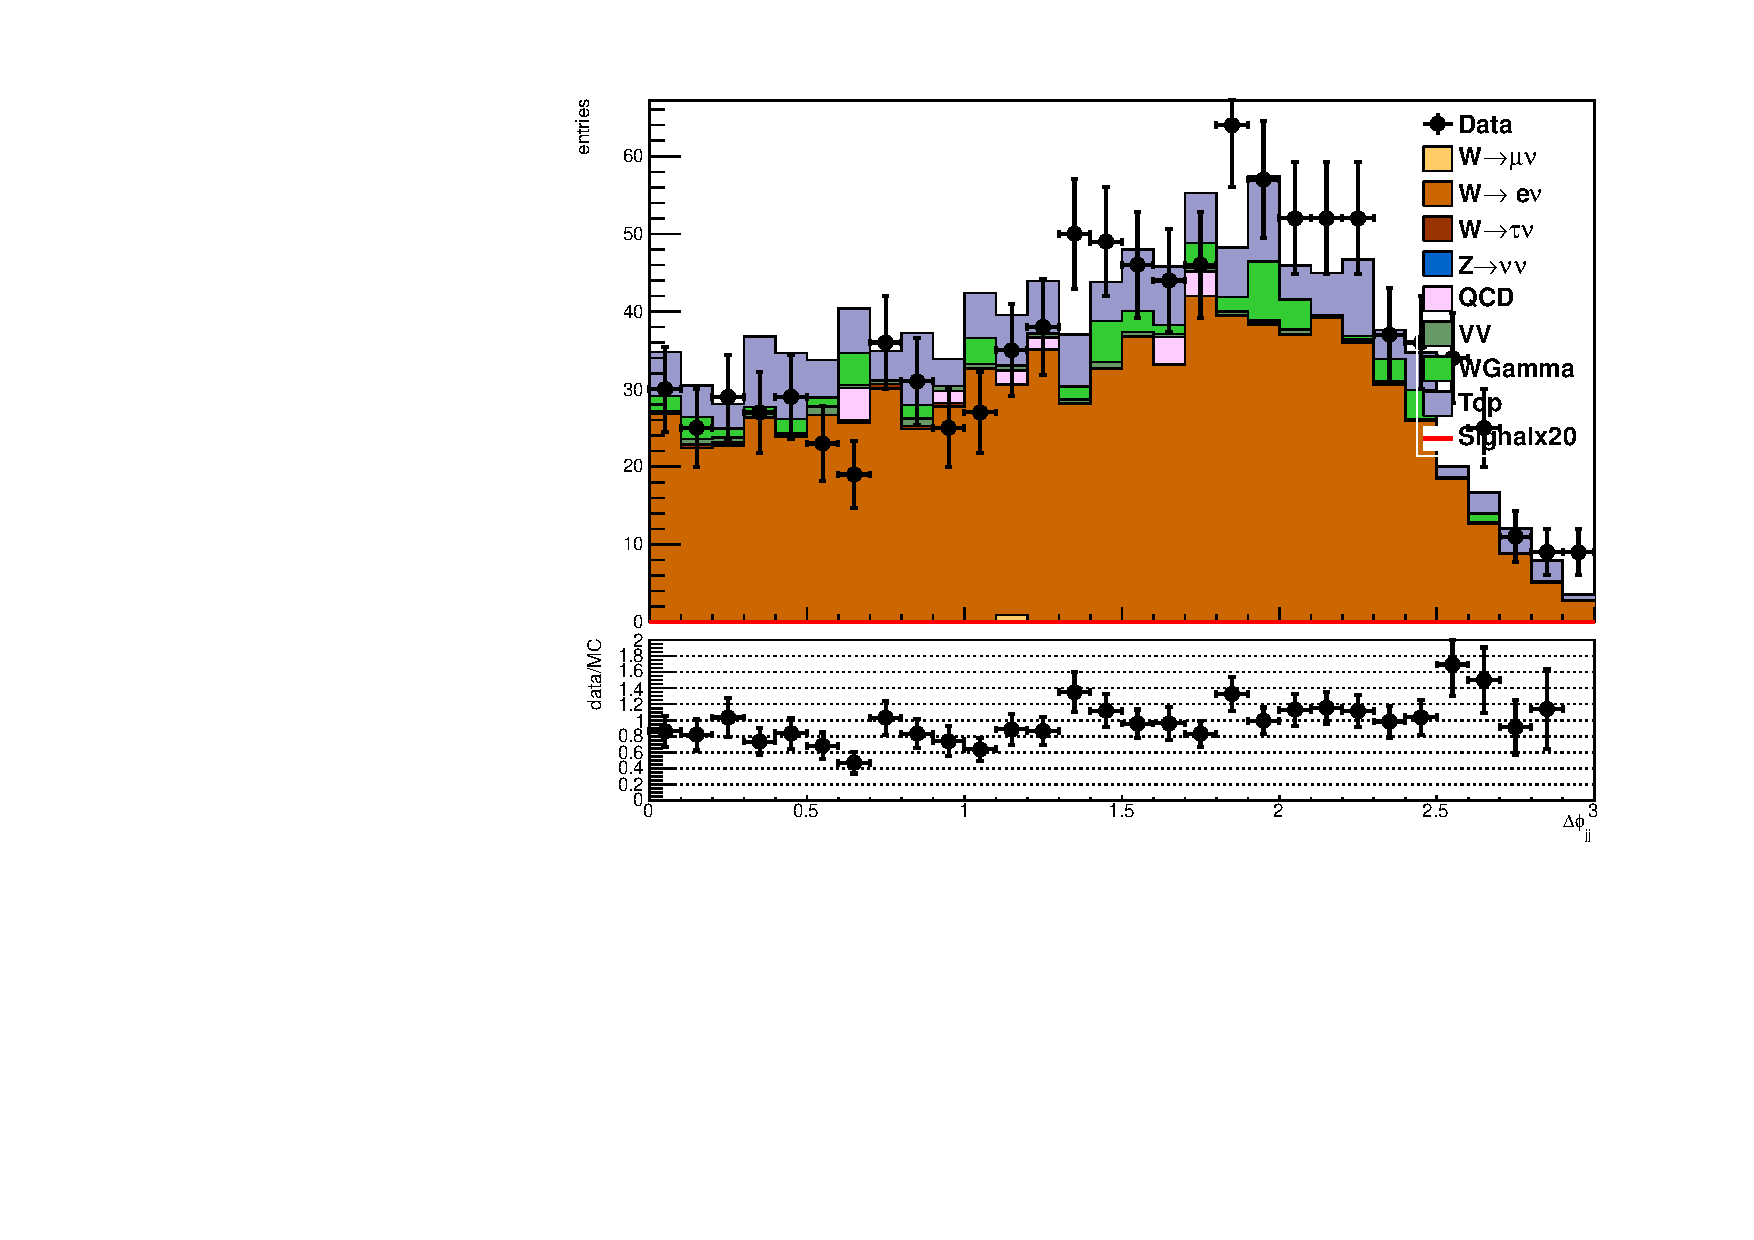
\includegraphics[width=\textwidth]{TalkPics/contplotsandpresel150914/output_contplots_alljetsmetdphicut10/enu_dijet_dphi.pdf}
    \end{block}
    \column{.5\textwidth}
    \begin{block}{Detajj}
      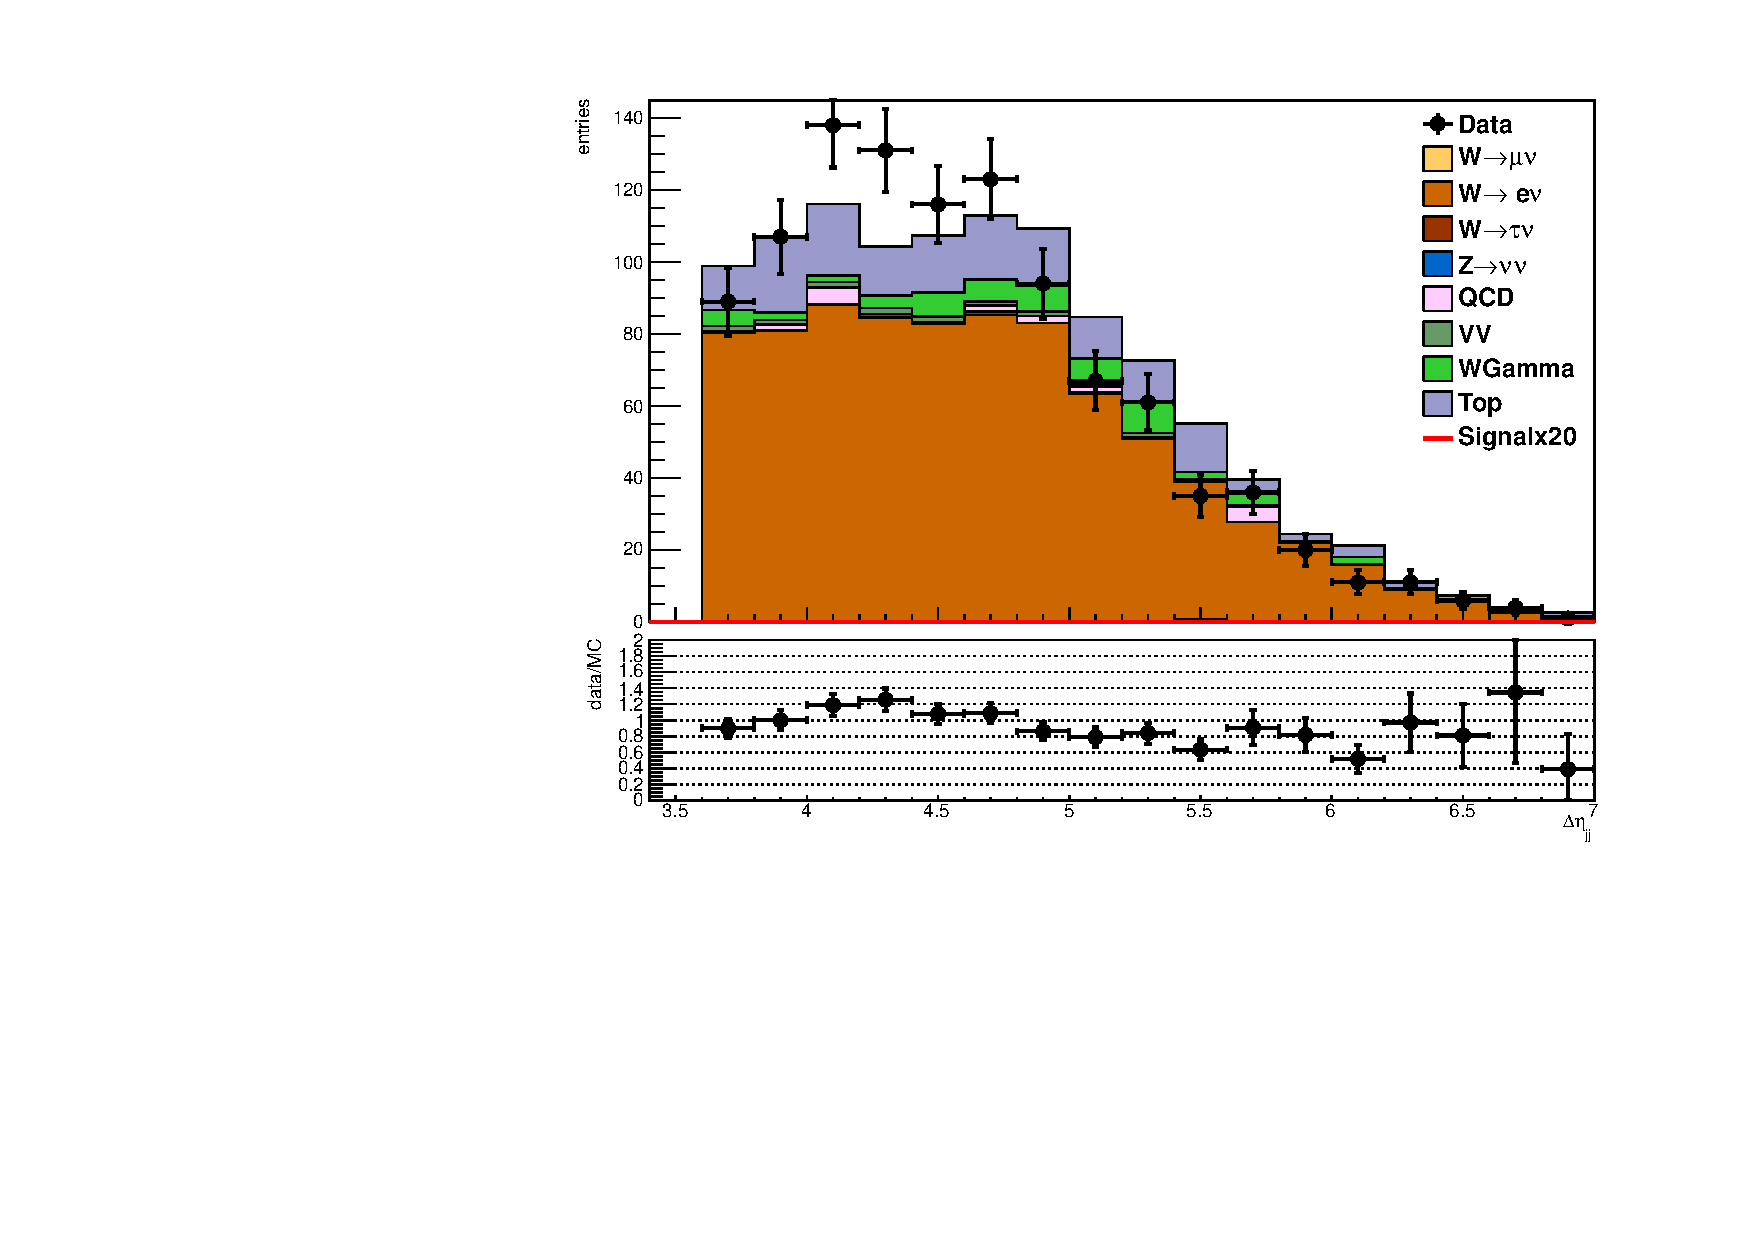
\includegraphics[width=\textwidth]{TalkPics/contplotsandpresel150914/output_contplots_alljetsmetdphicut10/enu_dijet_deta.pdf}
    \end{block}

  \end{columns}
\end{frame}

\begin{frame}
  \frametitle{New control plots - enu}
  \begin{columns}
    \column{.5\textwidth}
    \begin{block}{Leading jets-met mindphi}
      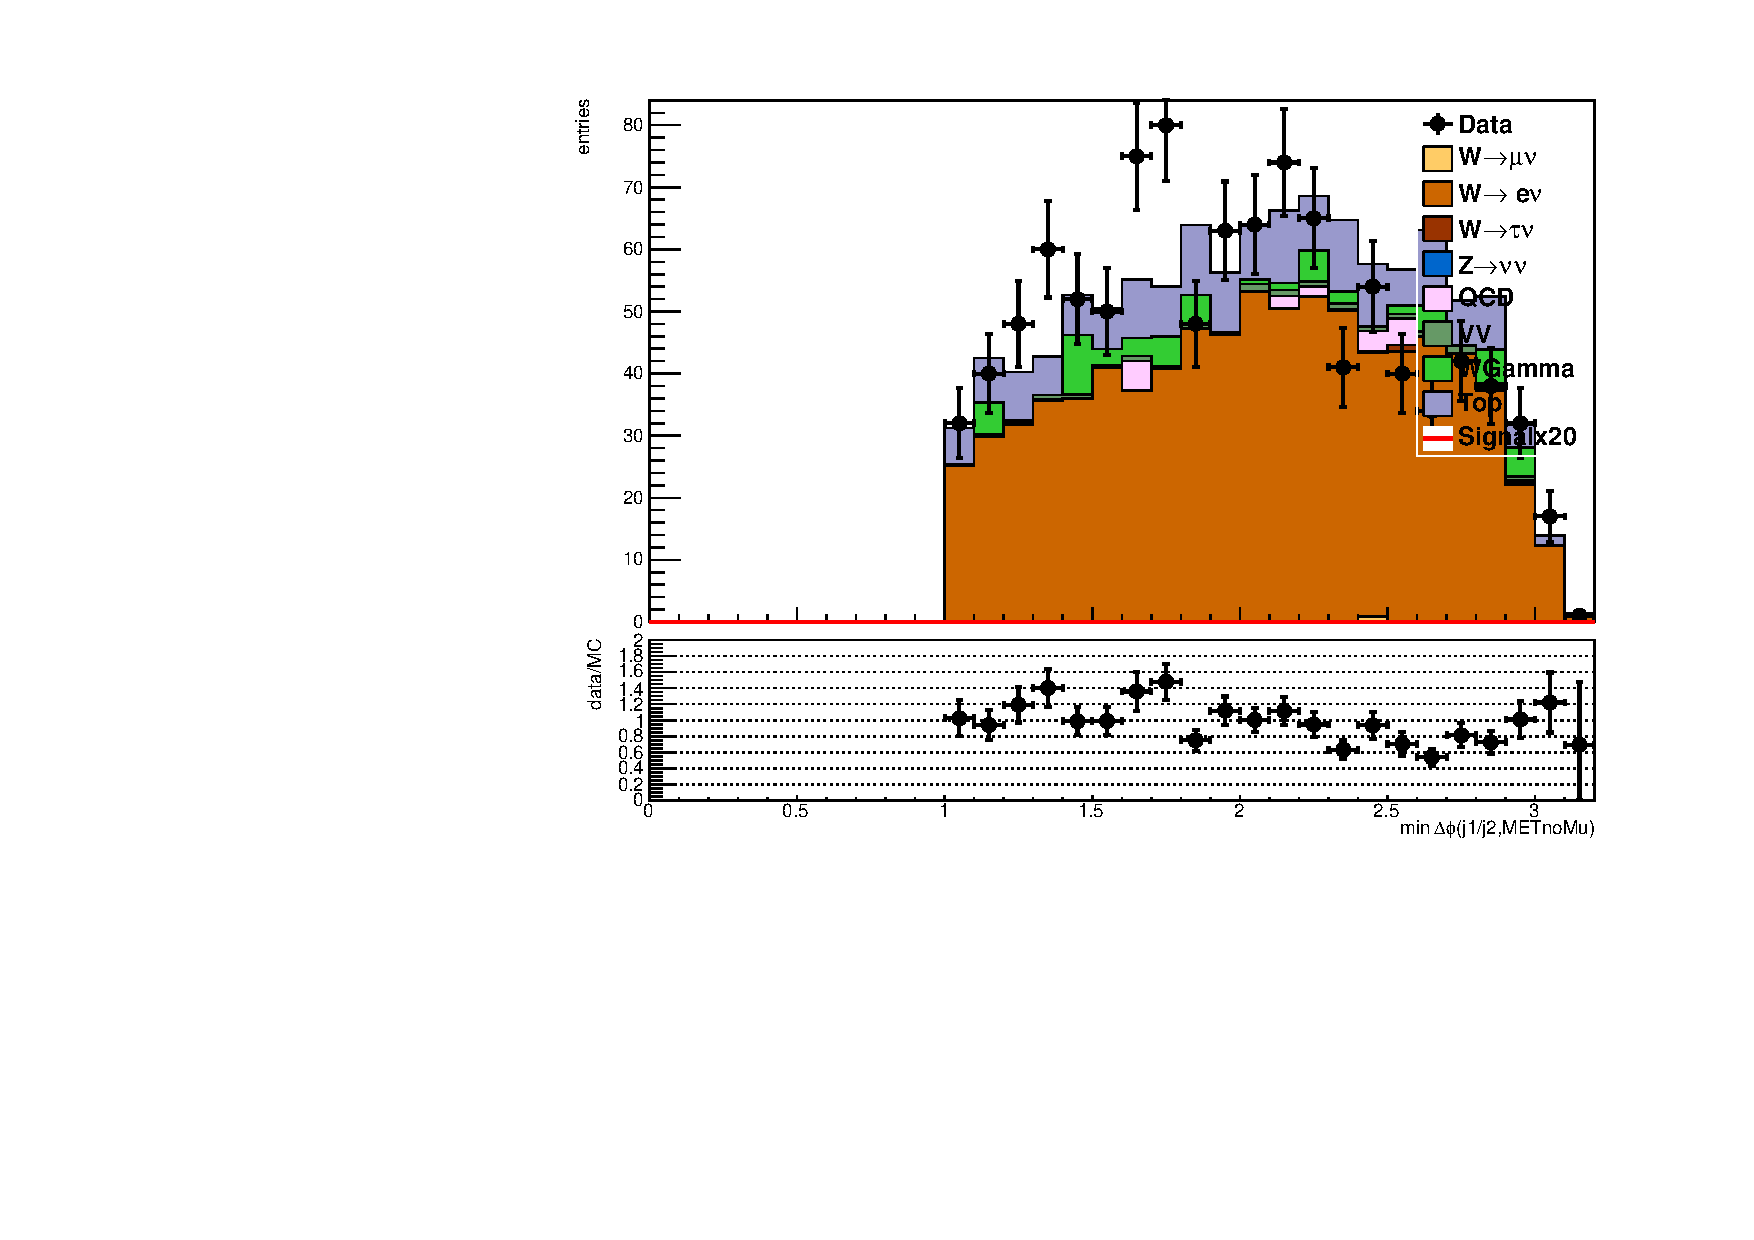
\includegraphics[width=\textwidth]{TalkPics/contplotsandpresel150914/output_contplots_alljetsmetdphicut10/enu_jetmetnomu_mindphi.pdf}
    \end{block}
    \column{.5\textwidth}
    \begin{block}{All jets-met mindphi}
      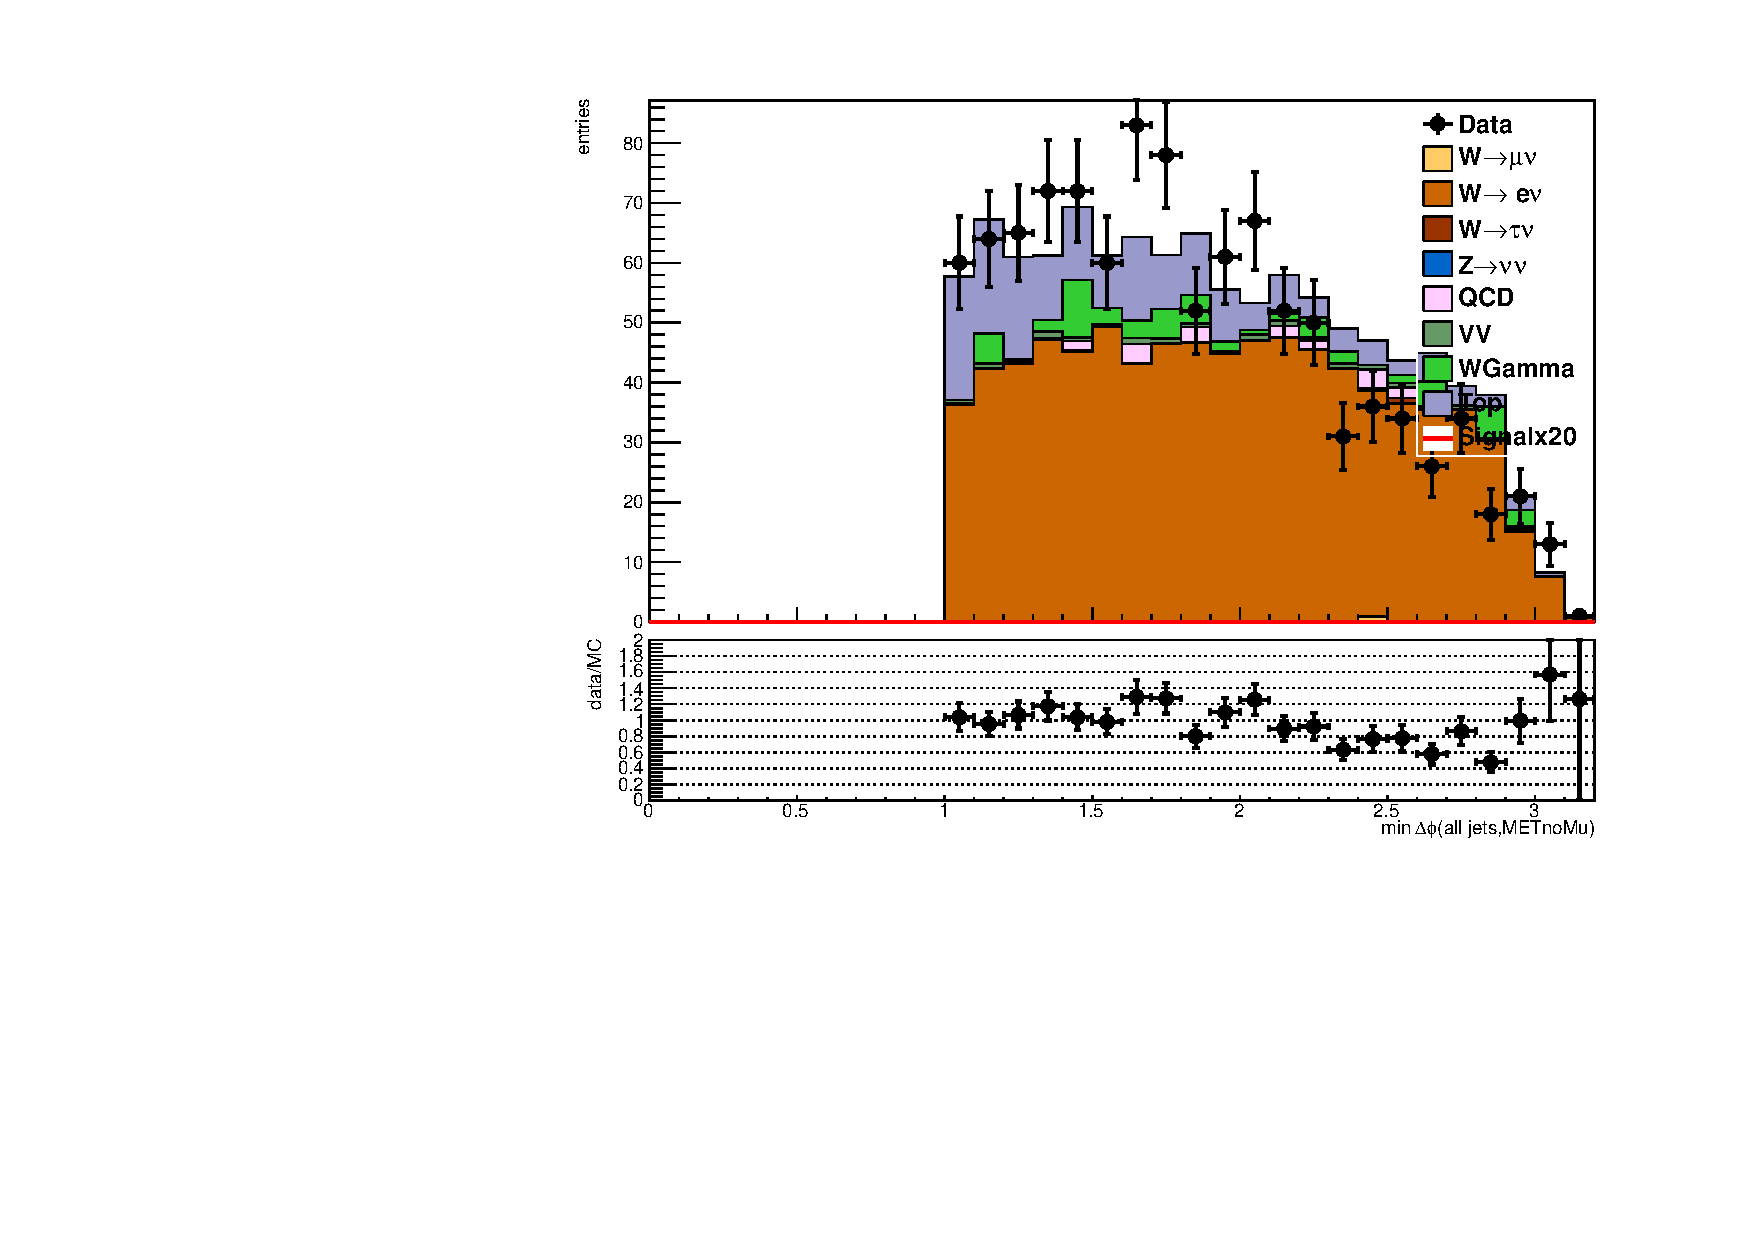
\includegraphics[width=\textwidth]{TalkPics/contplotsandpresel150914/output_contplots_alljetsmetdphicut10/enu_alljetsmetnomu_mindphi.pdf}
    \end{block}

  \end{columns}
\end{frame}

\begin{frame}
  \frametitle{New control plots - enu}
  \begin{columns}
    \column{.5\textwidth}
    \begin{block}{dijet-metnomu pt fraction}
      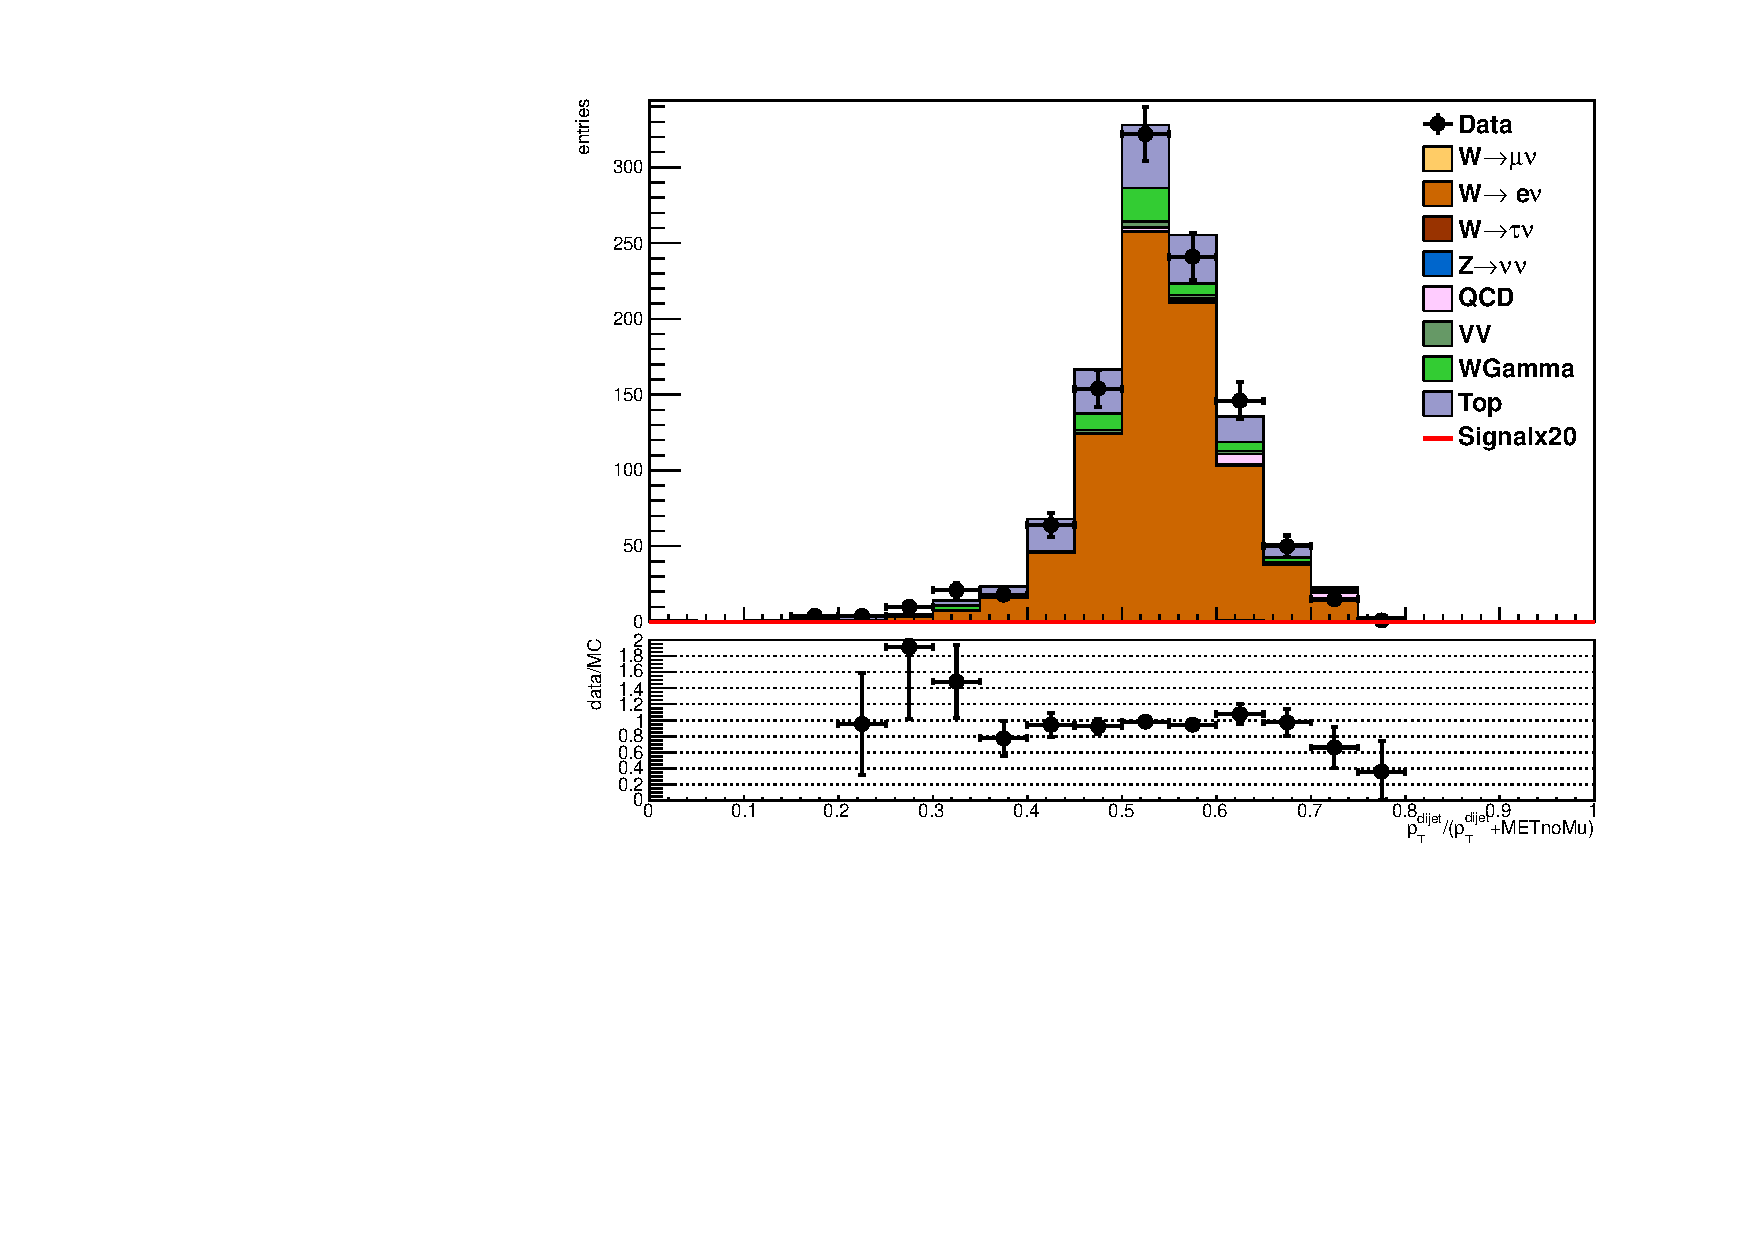
\includegraphics[width=\textwidth]{TalkPics/contplotsandpresel150914/output_contplots_alljetsmetdphicut10/enu_dijetmetnomu_ptfraction.pdf}
    \end{block}
  \end{columns}
\end{frame}

\begin{frame}
  \frametitle{New control plots - munu}
  \begin{columns}
    \column{.5\textwidth}
    \begin{block}{Jet 1 pt}
      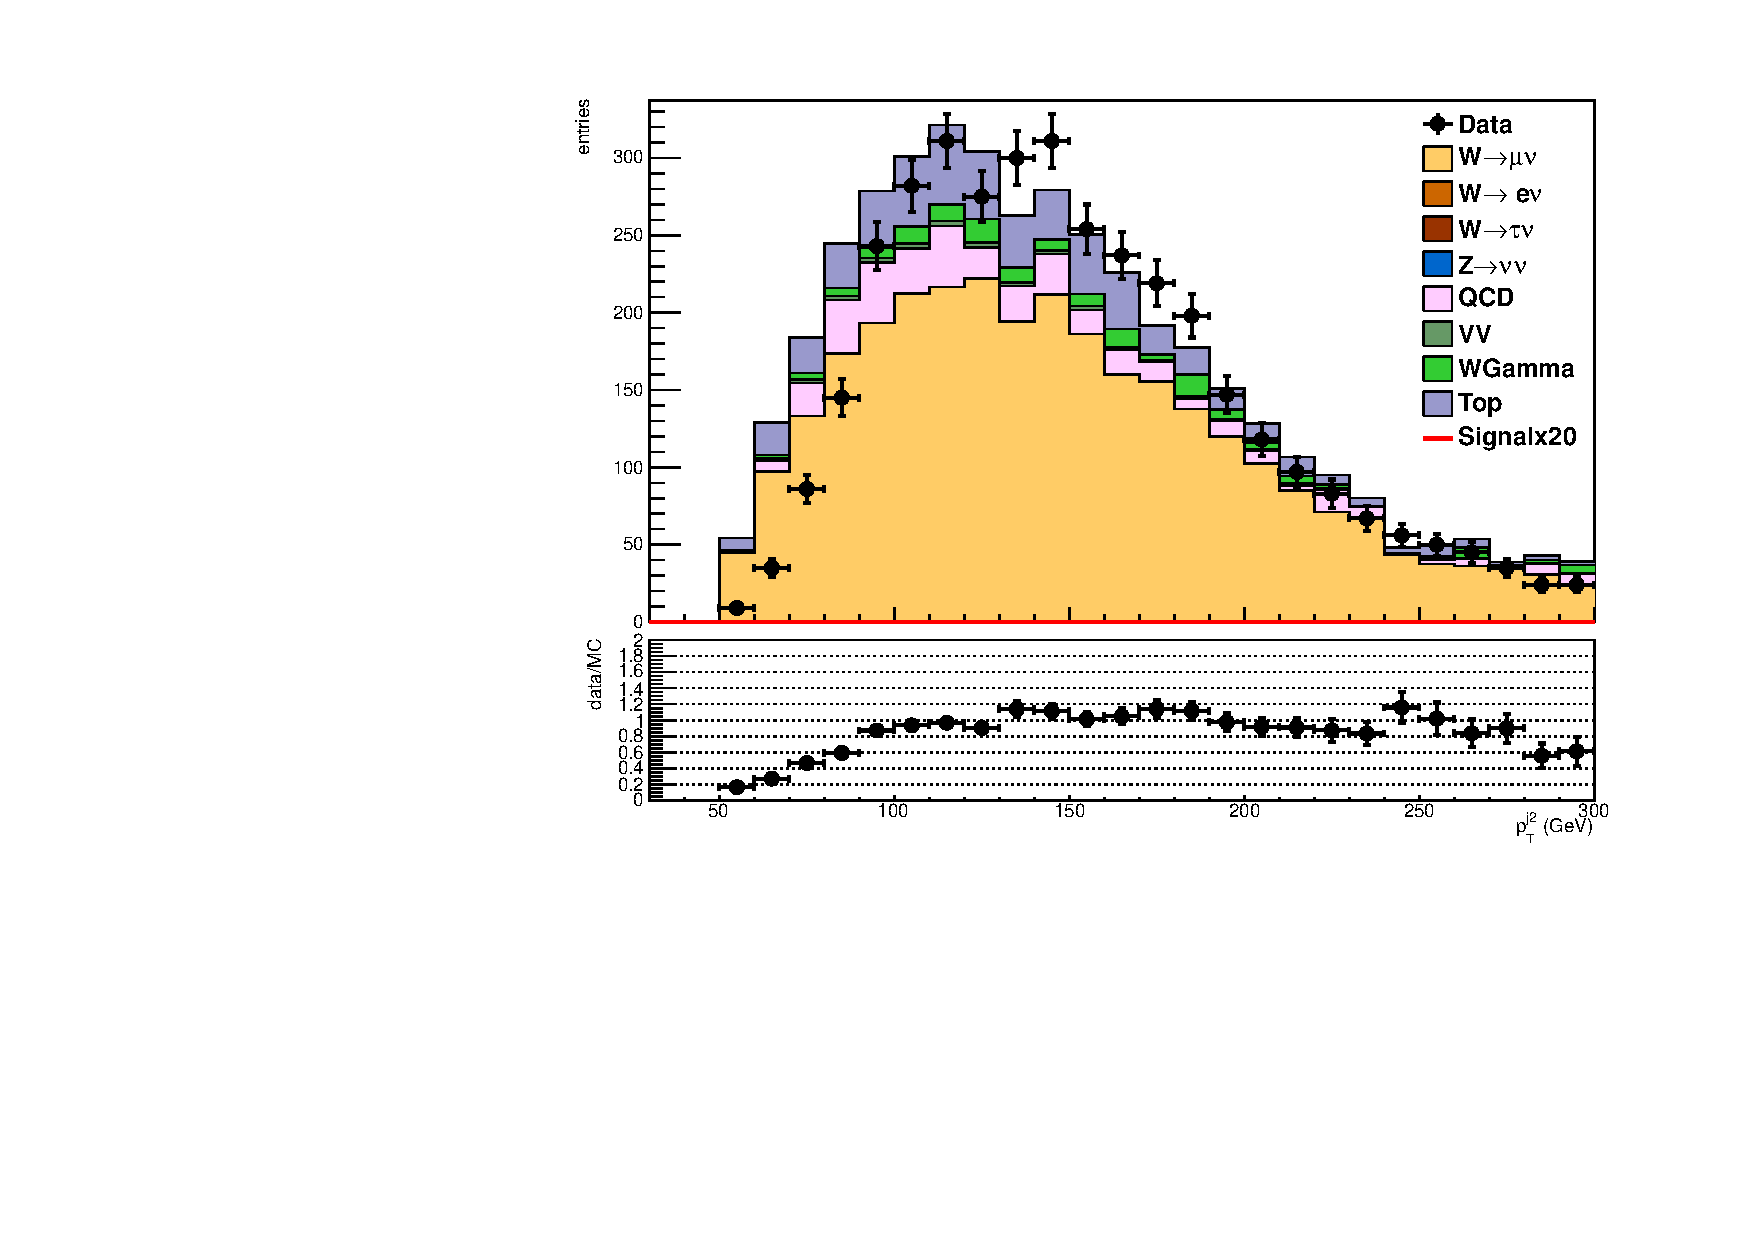
\includegraphics[width=\textwidth]{TalkPics/contplotsandpresel150914/output_contplots_alljetsmetdphicut10/munu_jet1_pt.pdf}
    \end{block}
    \column{.5\textwidth}
    \begin{block}{Jet 2 pt}
      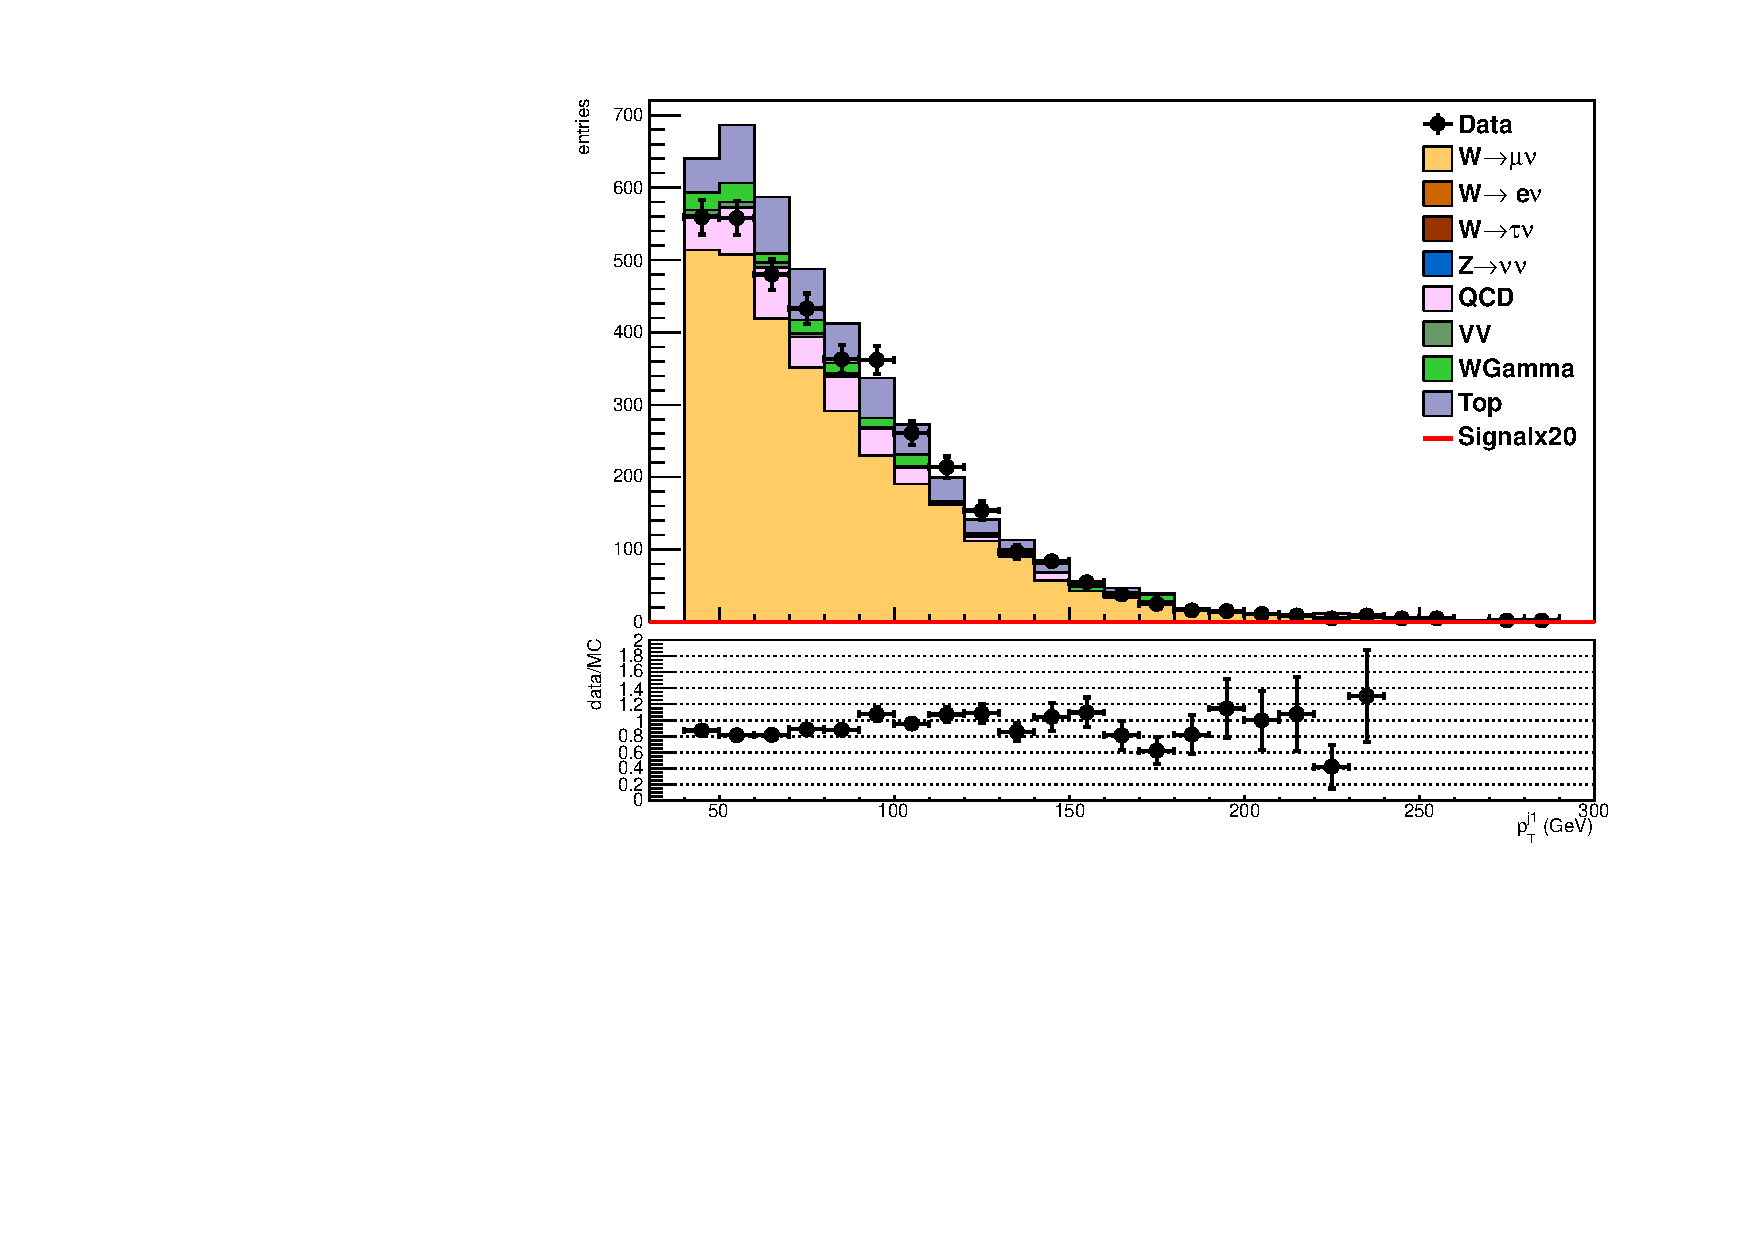
\includegraphics[width=\textwidth]{TalkPics/contplotsandpresel150914/output_contplots_alljetsmetdphicut10/munu_jet2_pt.pdf}
    \end{block}

  \end{columns}
\end{frame}

\begin{frame}
  \frametitle{New control plots - munu}
  \begin{columns}
    \column{.5\textwidth}
    \begin{block}{METnomu}
      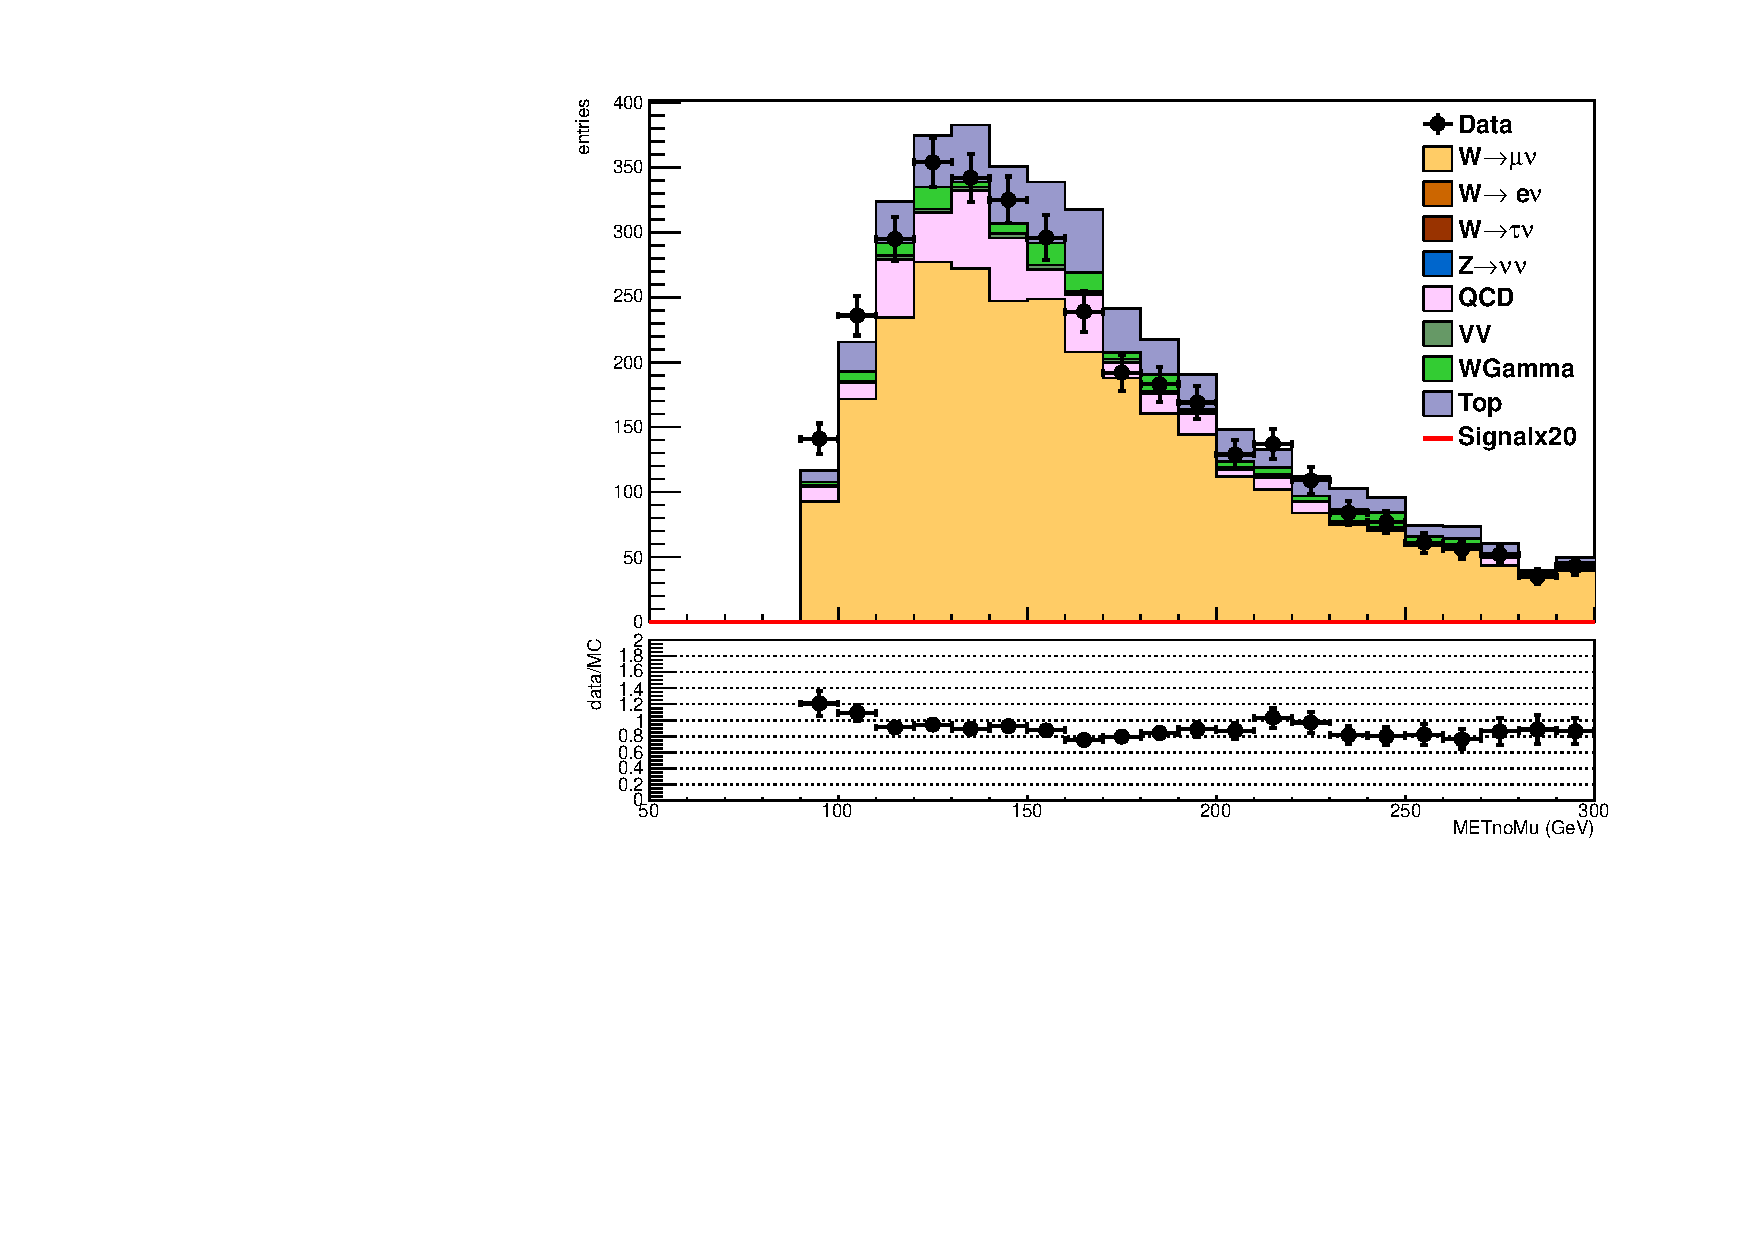
\includegraphics[width=\textwidth]{TalkPics/contplotsandpresel150914/output_contplots_alljetsmetdphicut10/munu_metnomuons.pdf}
    \end{block}
    \column{.5\textwidth}
    \begin{block}{METnomusig}
      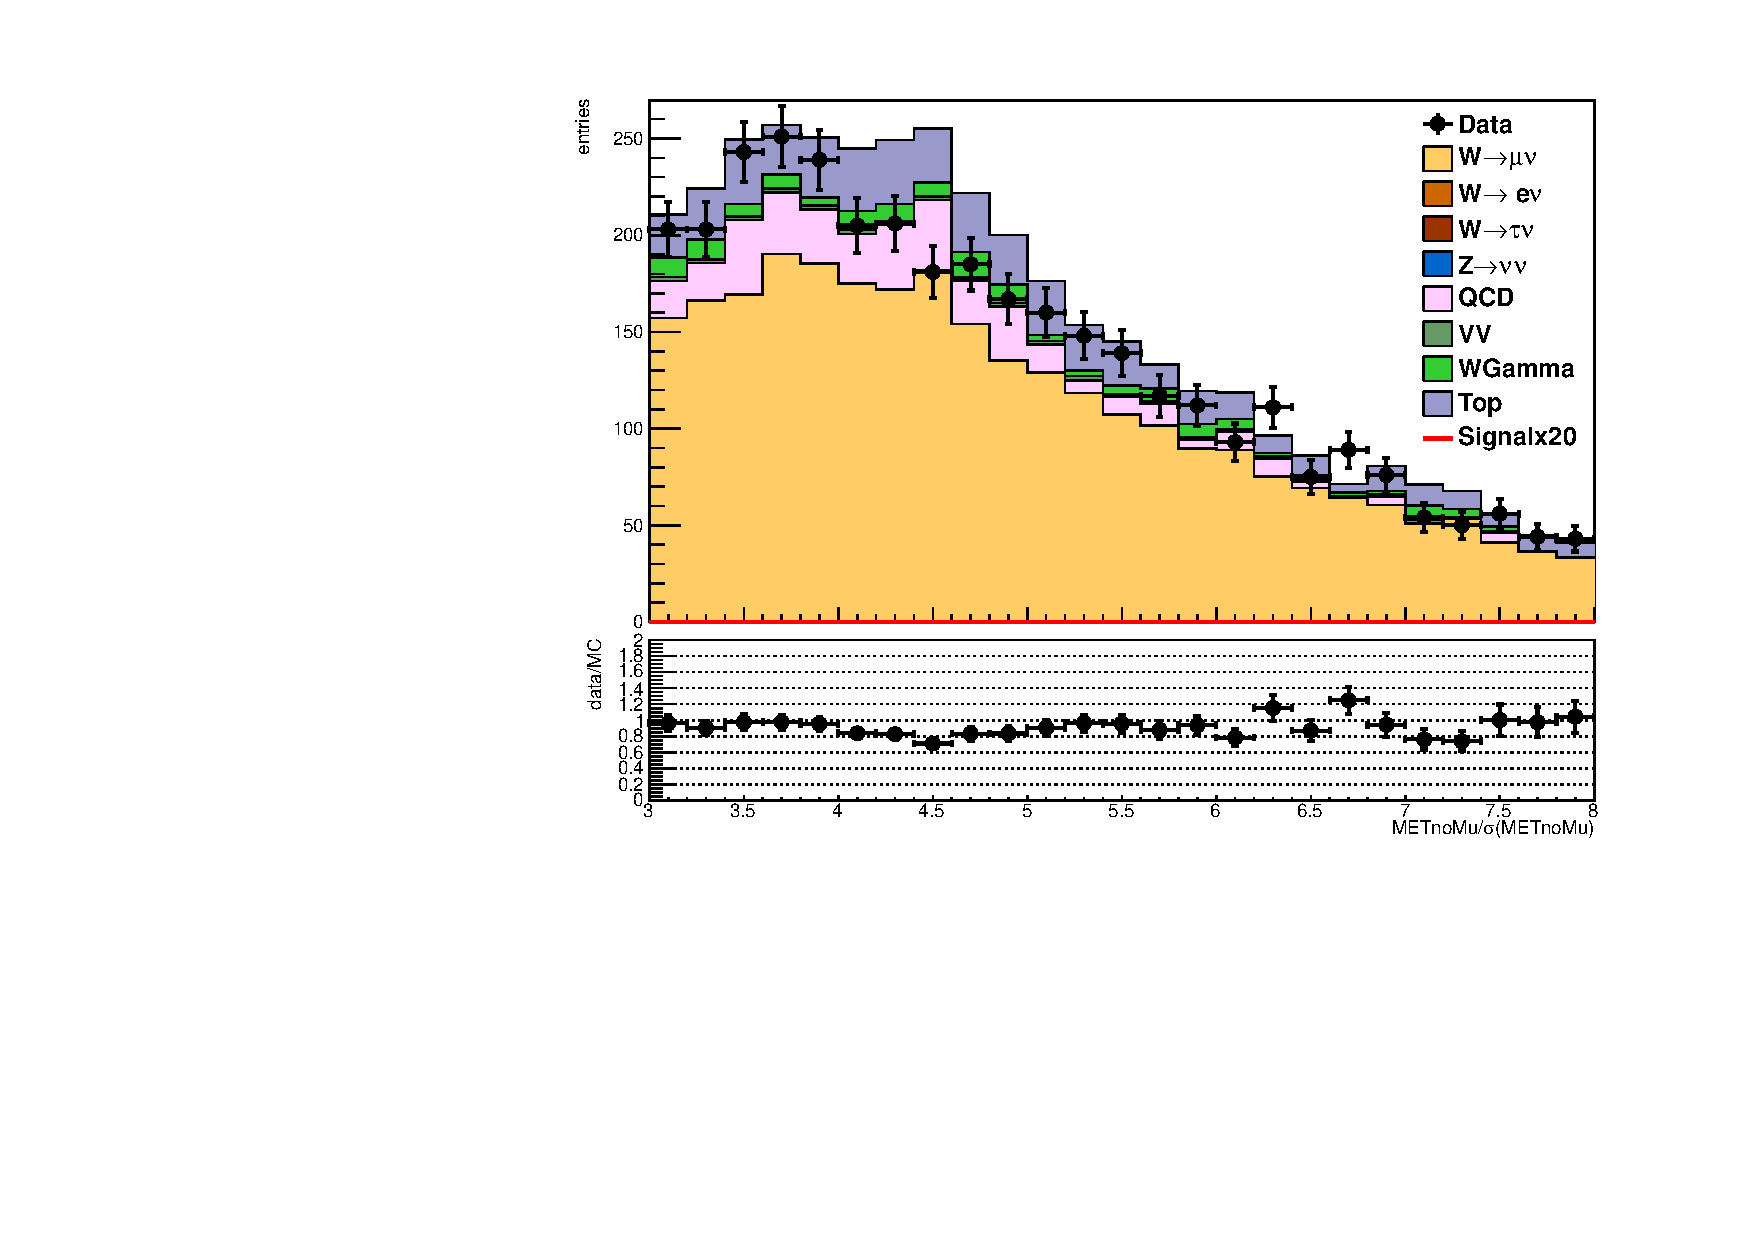
\includegraphics[width=\textwidth]{TalkPics/contplotsandpresel150914/output_contplots_alljetsmetdphicut10/munu_metnomu_significance.pdf}
    \end{block}

  \end{columns}
\end{frame}

\begin{frame}
  \frametitle{New control plots - munu}
  \begin{columns}
    \column{.5\textwidth}
    \begin{block}{Mjj}
      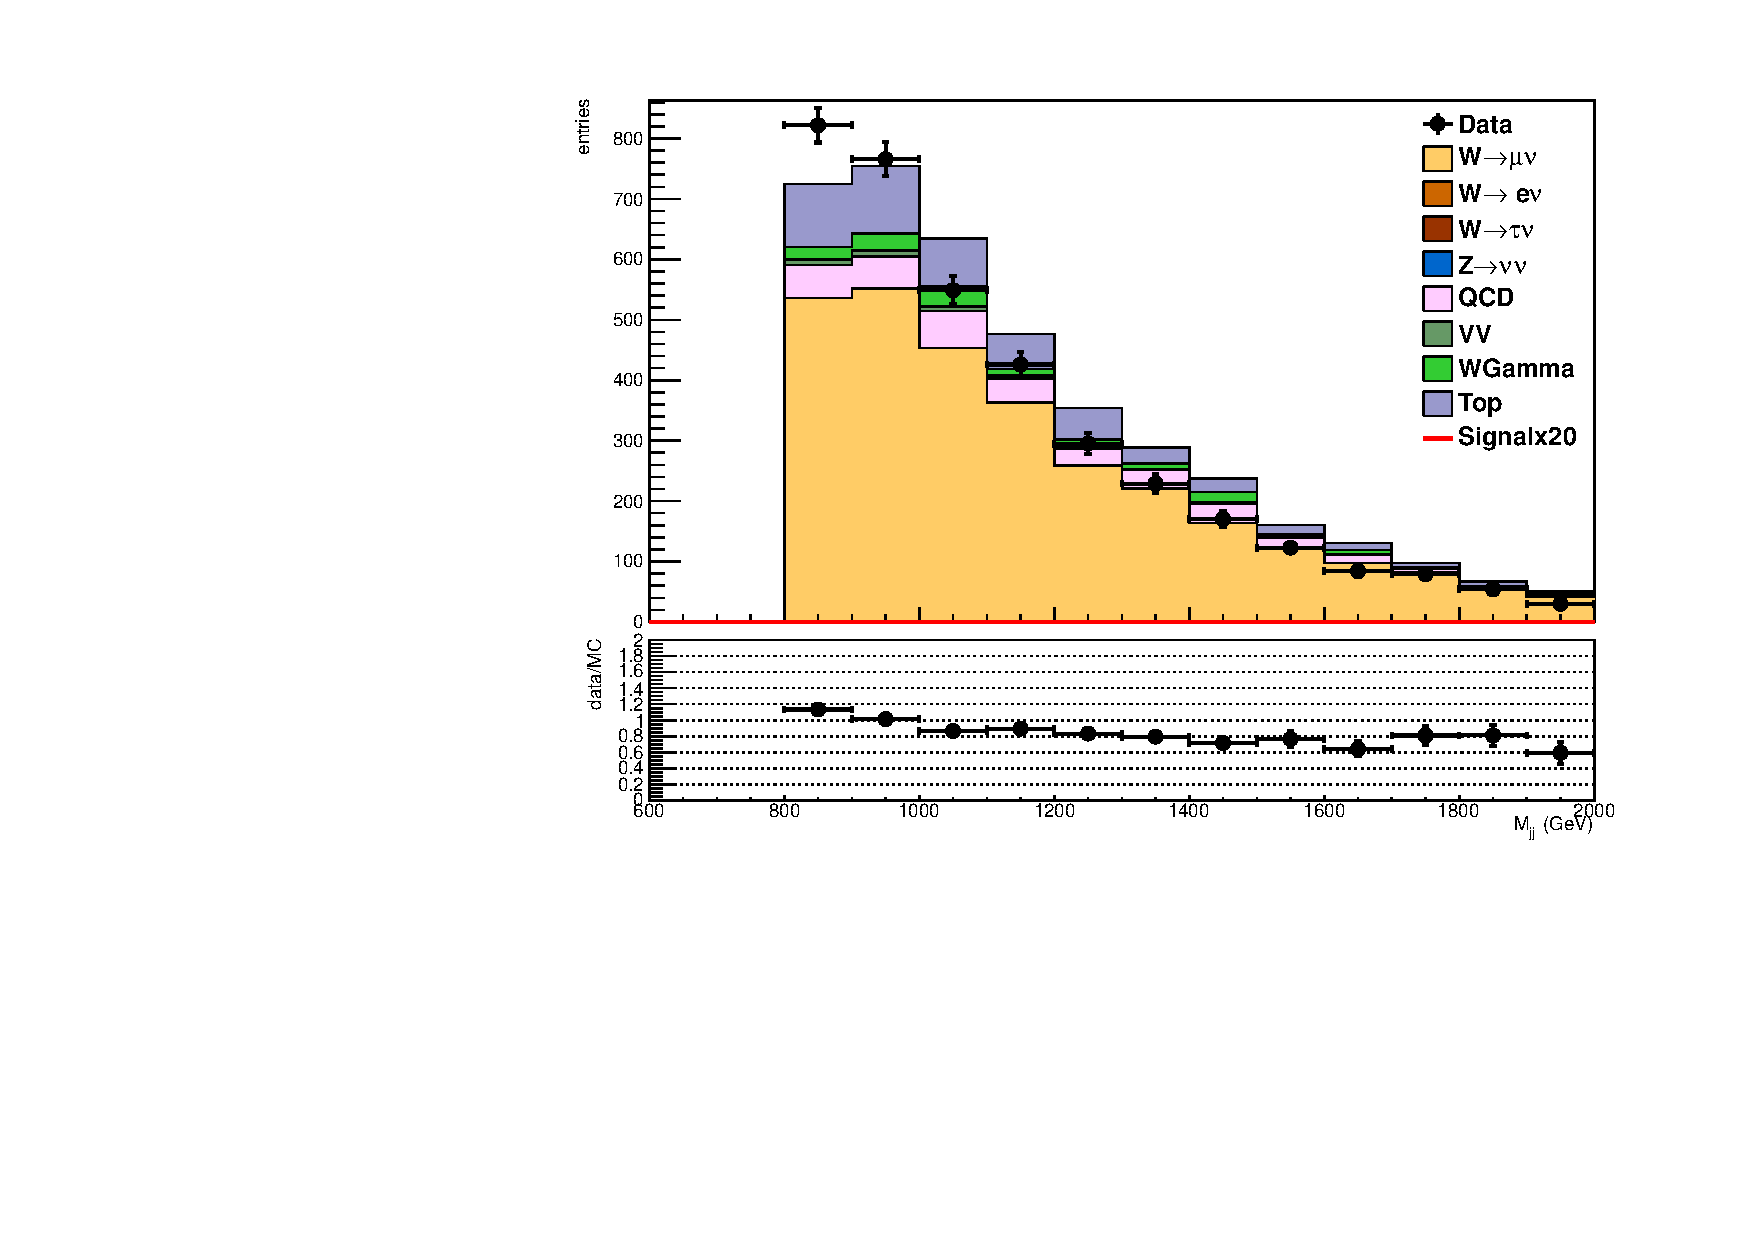
\includegraphics[width=\textwidth]{TalkPics/contplotsandpresel150914/output_contplots_alljetsmetdphicut10/munu_dijet_M.pdf}
    \end{block}
    \column{.5\textwidth}
    \begin{block}{mt}
      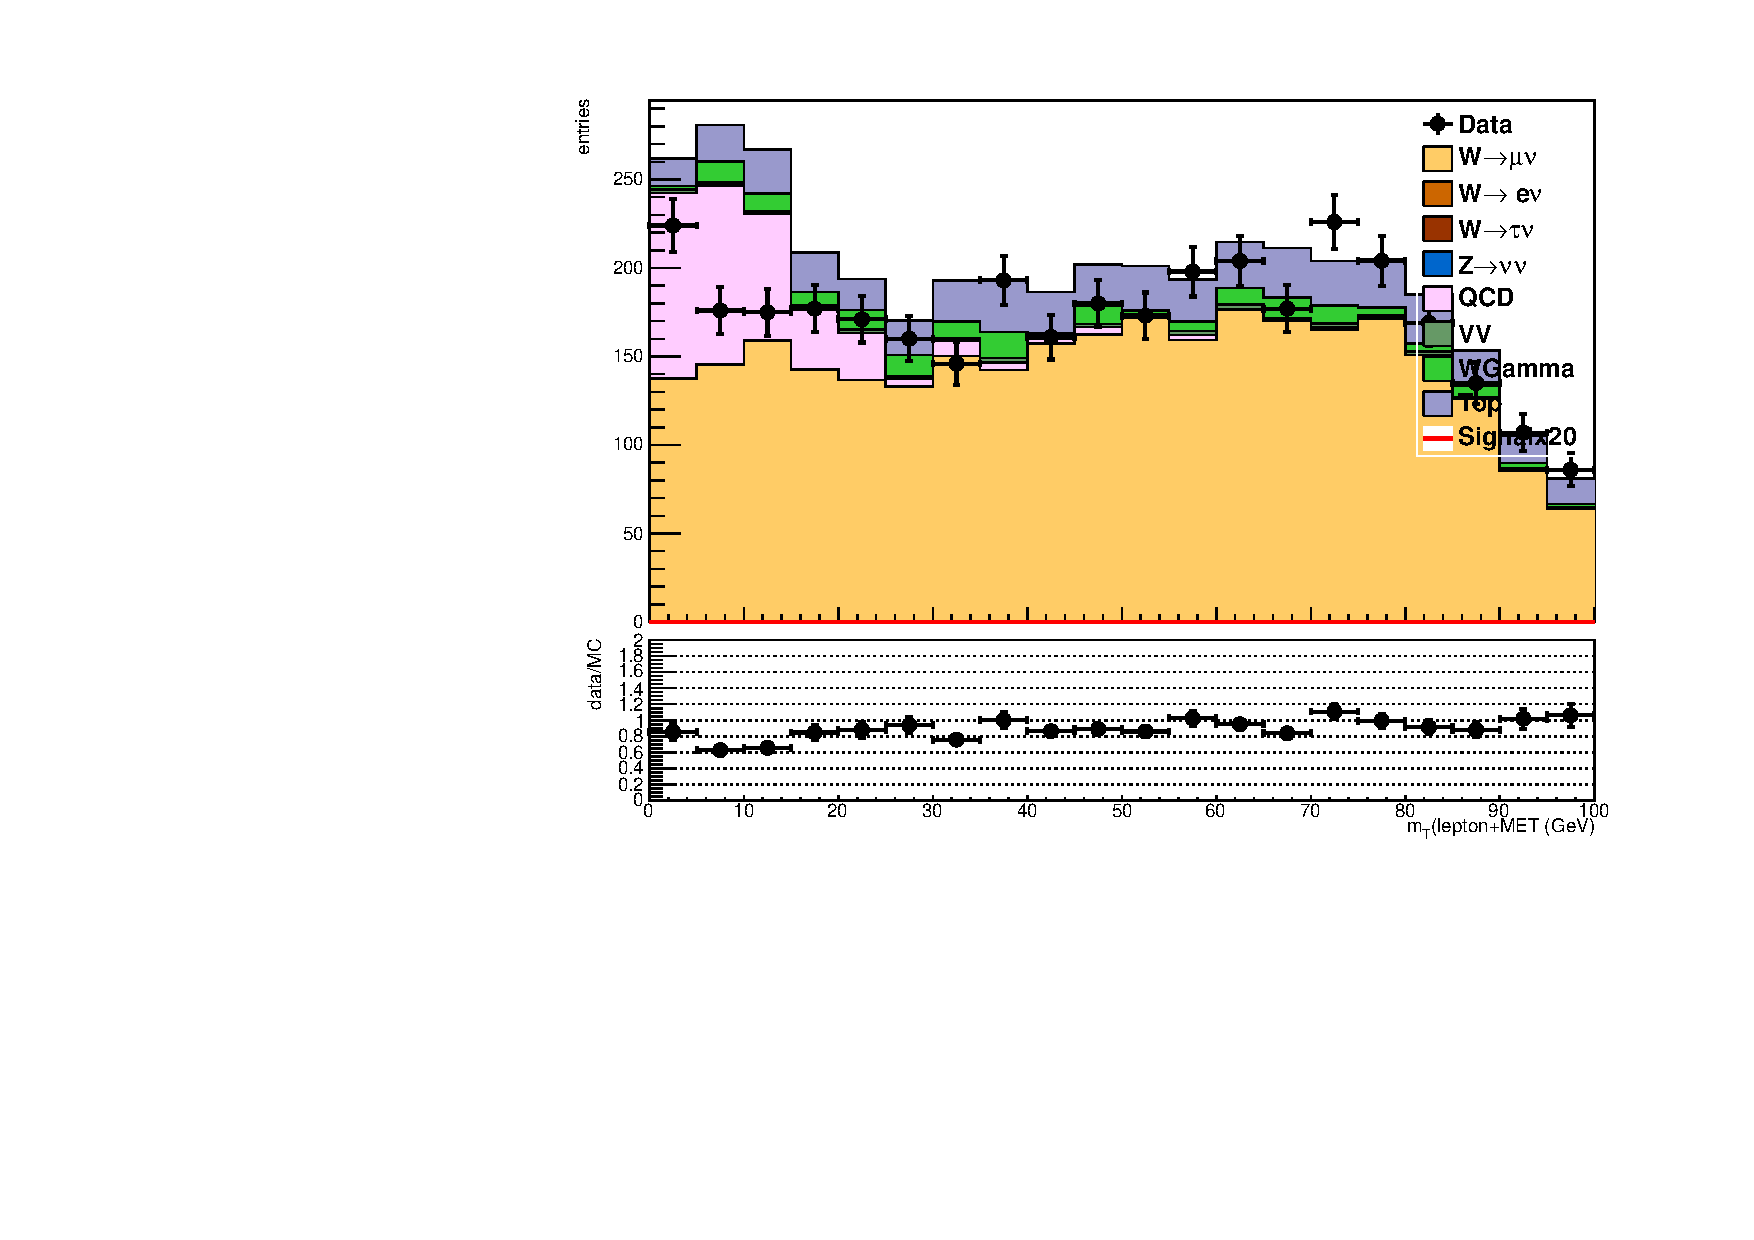
\includegraphics[width=\textwidth]{TalkPics/contplotsandpresel150914/output_contplots_alljetsmetdphicut10/munu_lep_mt.pdf}
    \end{block}
  \end{columns}
\end{frame}

\begin{frame}
  \frametitle{New control plots - munu}
  \begin{columns}
    \column{.5\textwidth}
    \begin{block}{Dijet Dphi}
      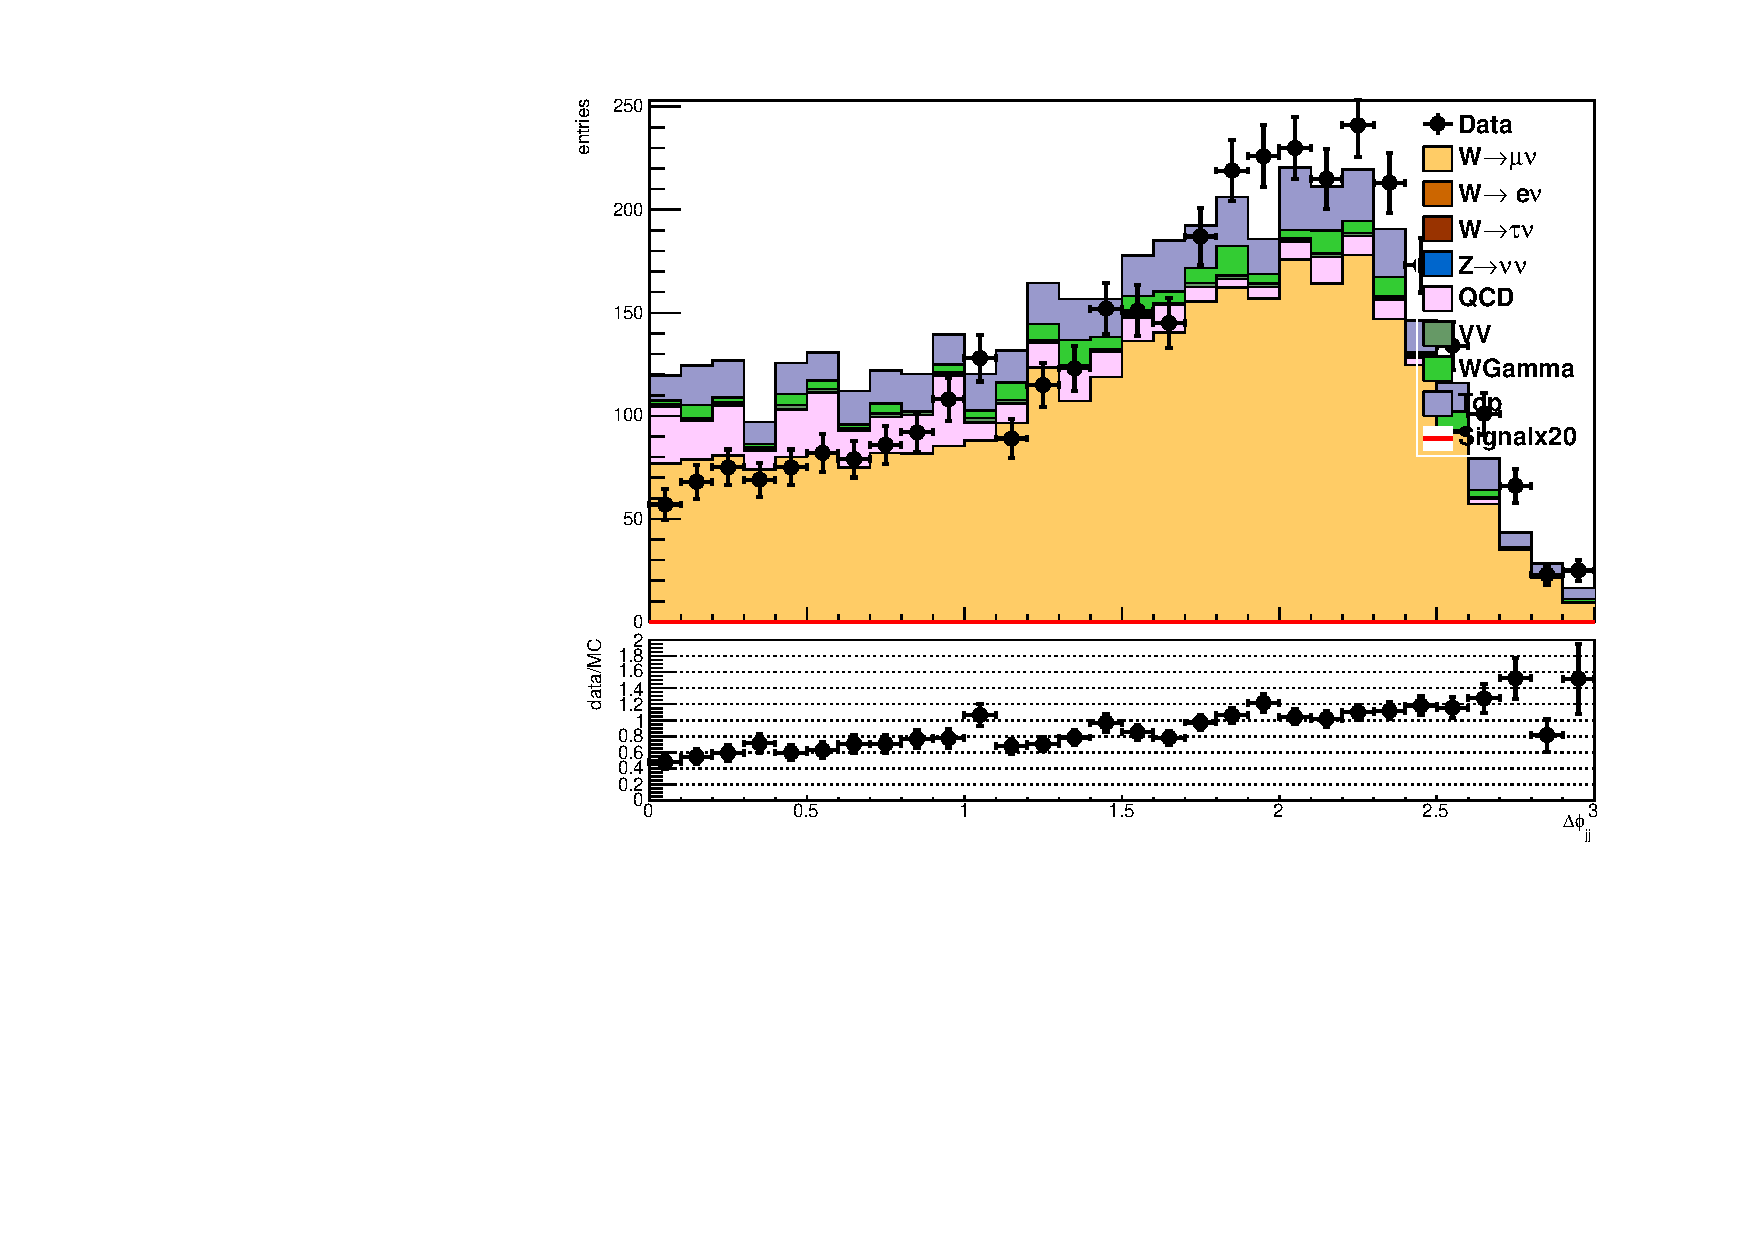
\includegraphics[width=\textwidth]{TalkPics/contplotsandpresel150914/output_contplots_alljetsmetdphicut10/munu_dijet_dphi.pdf}
    \end{block}
    \column{.5\textwidth}
    \begin{block}{Detajj}
      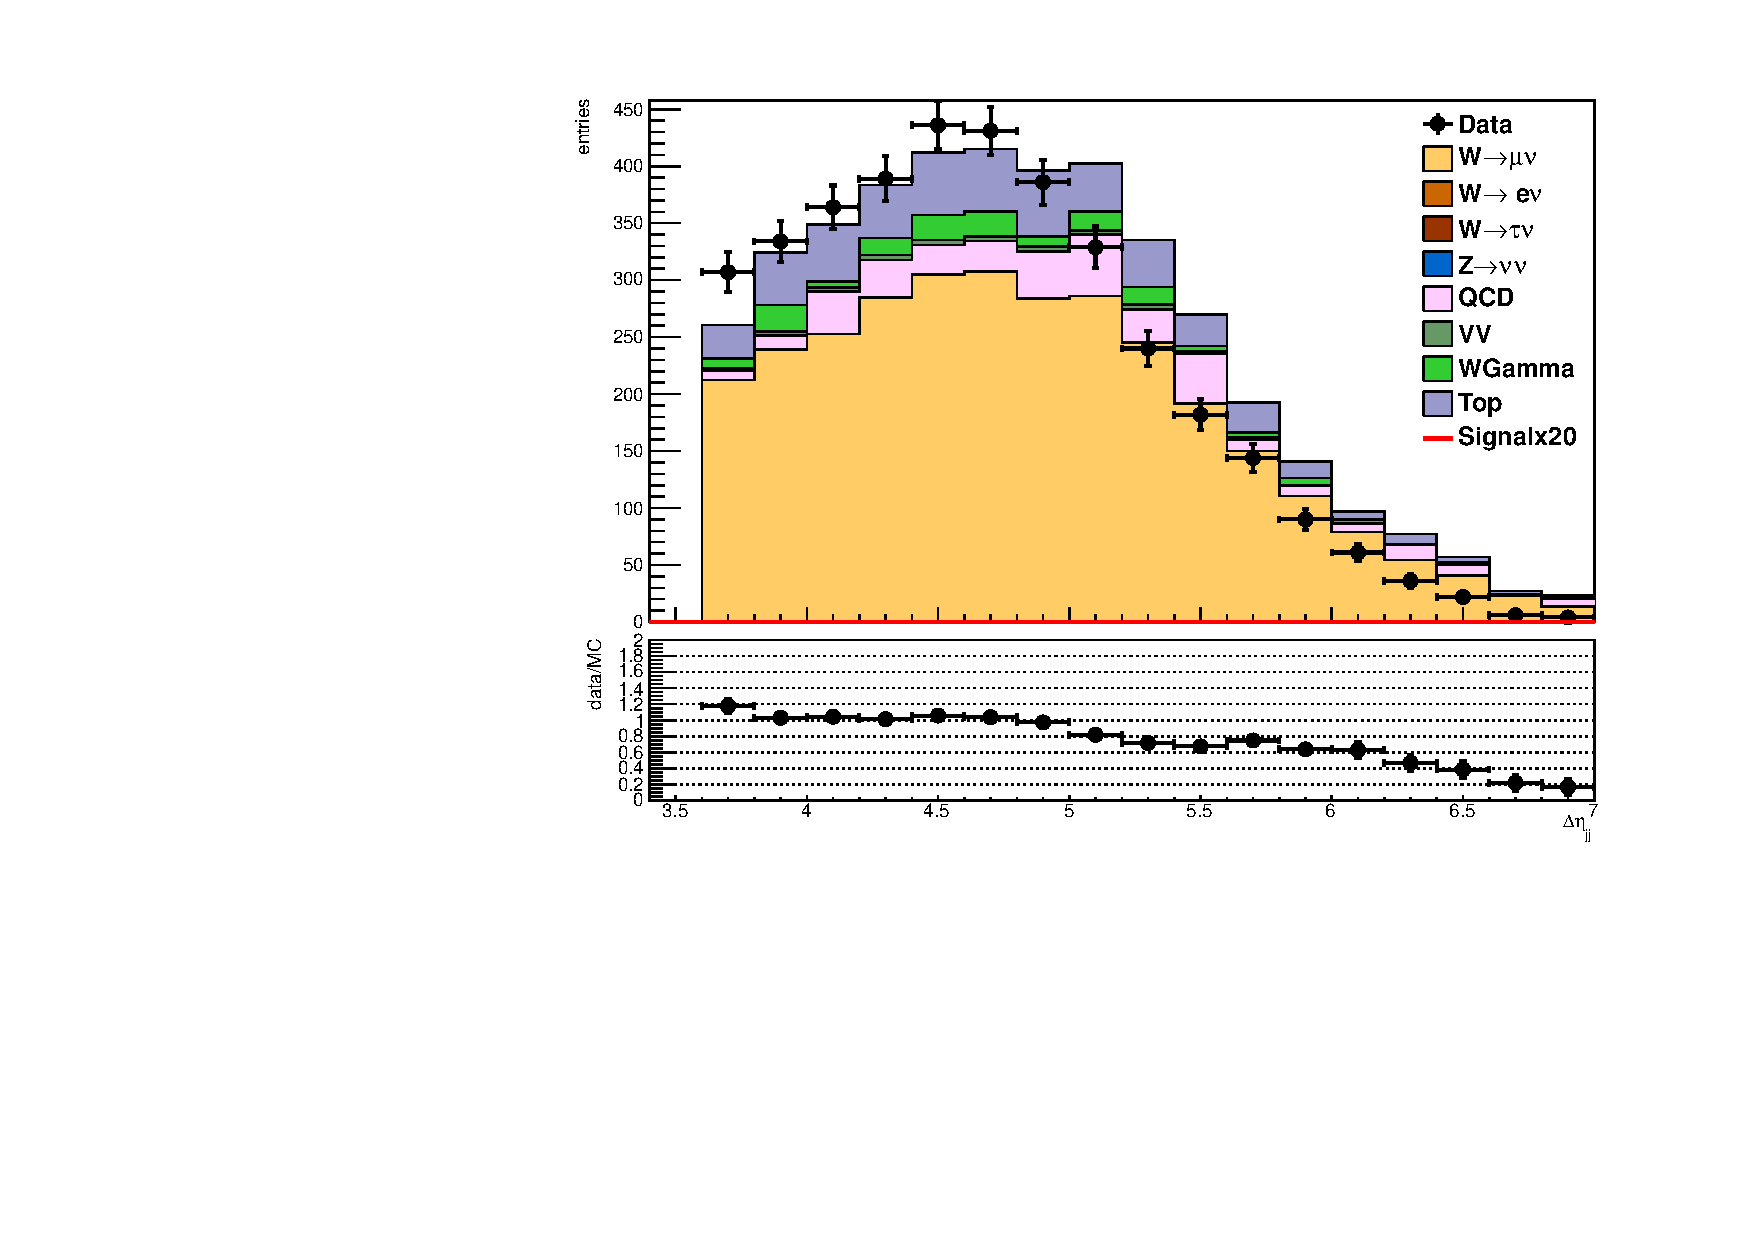
\includegraphics[width=\textwidth]{TalkPics/contplotsandpresel150914/output_contplots_alljetsmetdphicut10/munu_dijet_deta.pdf}
    \end{block}

  \end{columns}
\end{frame}

\begin{frame}
  \frametitle{New control plots - munu}
  \begin{columns}
    \column{.5\textwidth}
    \begin{block}{Leading jets-met mindphi}
      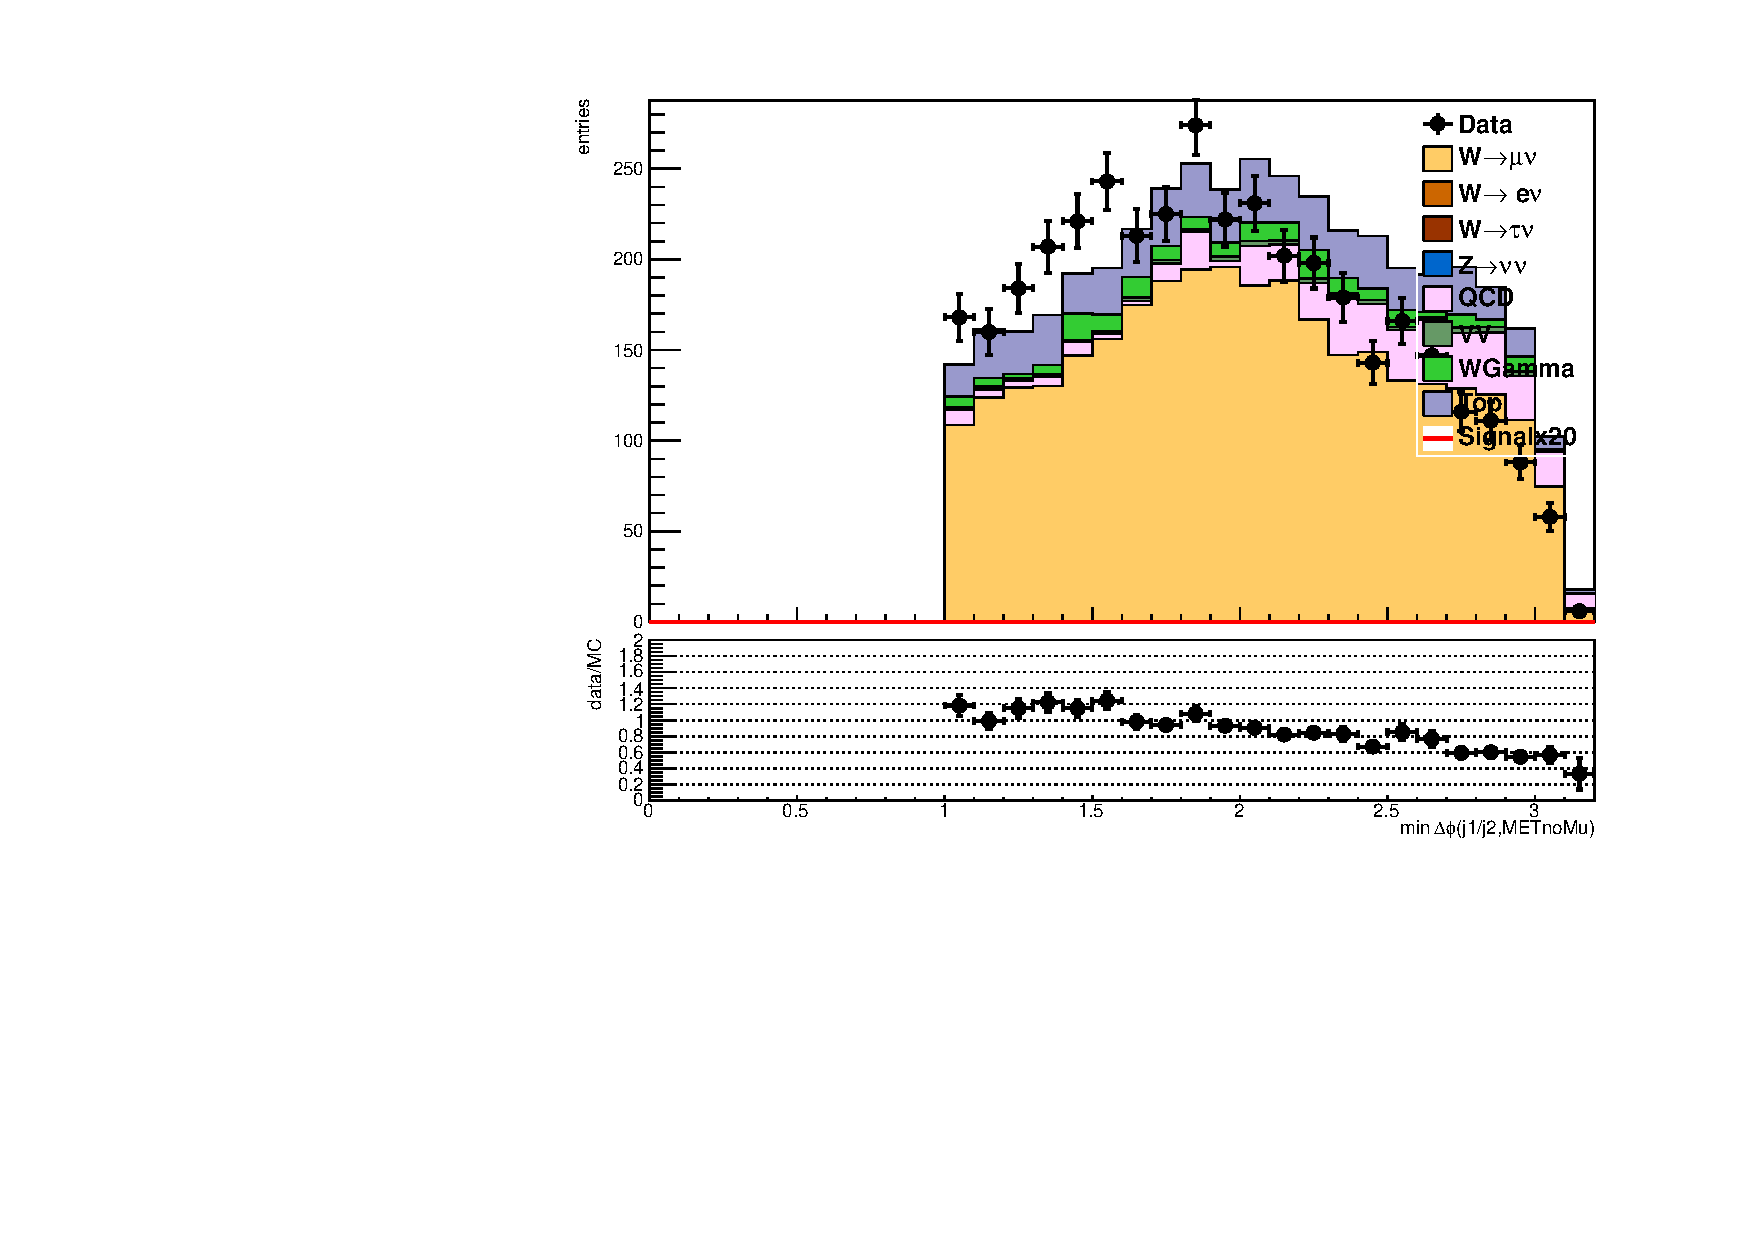
\includegraphics[width=\textwidth]{TalkPics/contplotsandpresel150914/output_contplots_alljetsmetdphicut10/munu_jetmetnomu_mindphi.pdf}
    \end{block}
    \column{.5\textwidth}
    \begin{block}{All jets-met mindphi}
      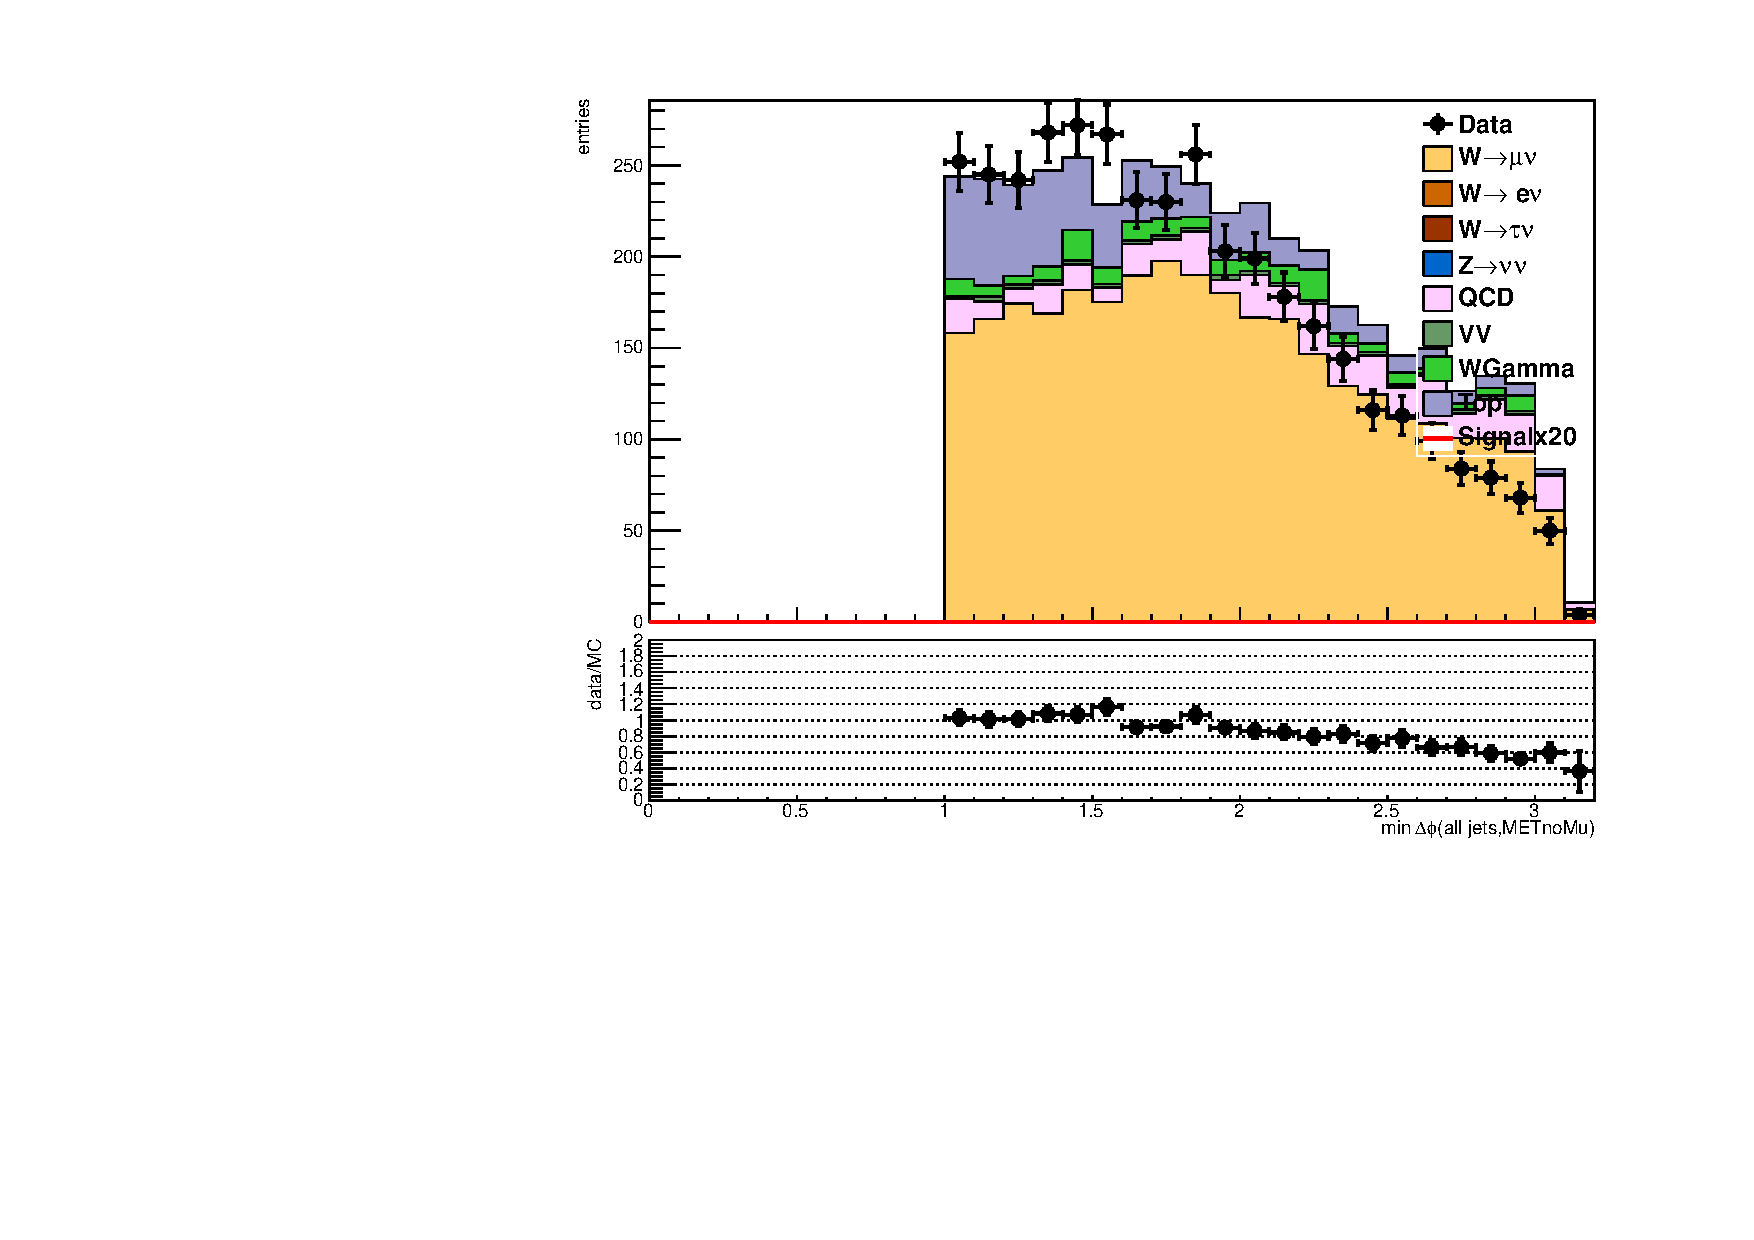
\includegraphics[width=\textwidth]{TalkPics/contplotsandpresel150914/output_contplots_alljetsmetdphicut10/munu_alljetsmetnomu_mindphi.pdf}
    \end{block}

  \end{columns}
\end{frame}

\begin{frame}
  \frametitle{New control plots - munu}
  \begin{columns}
    \column{.5\textwidth}
    \begin{block}{dijet-metnomu pt fraction}
      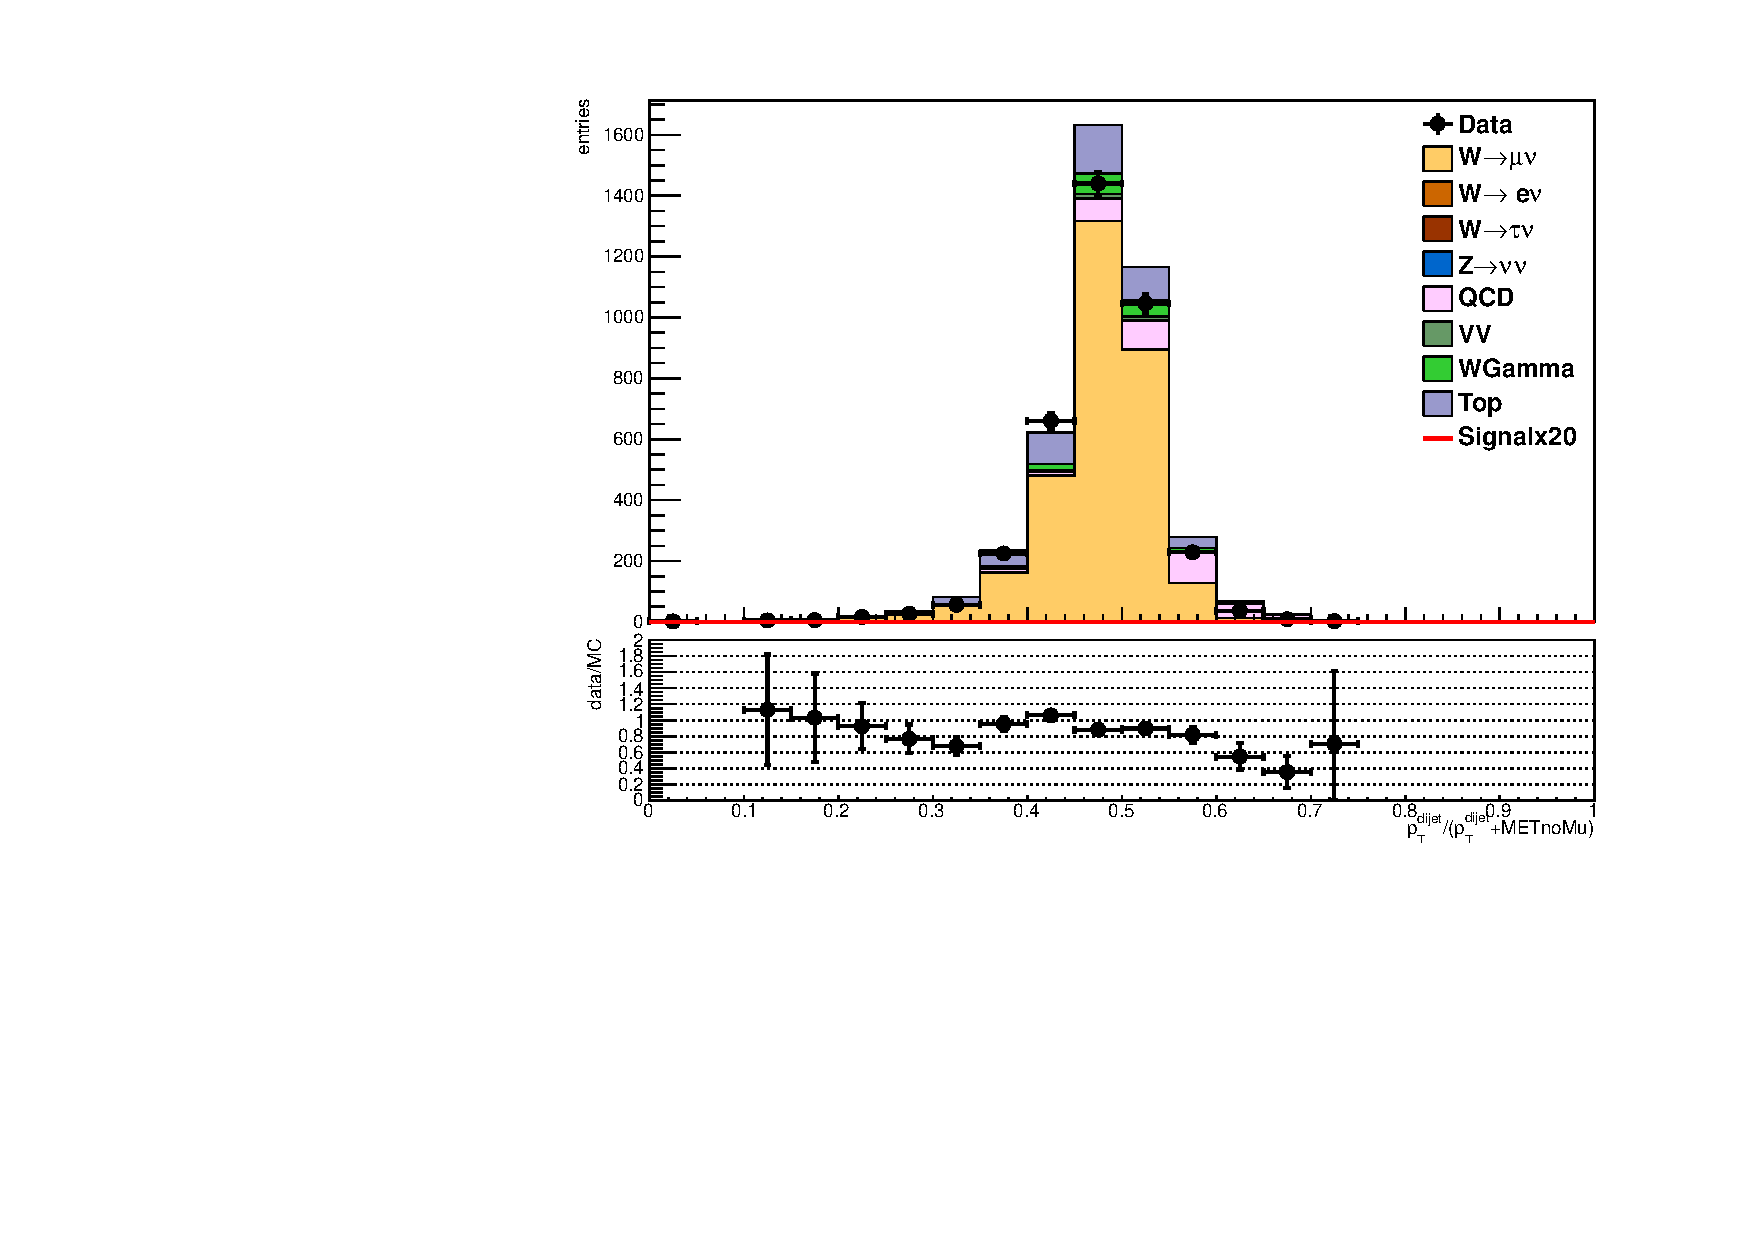
\includegraphics[width=\textwidth]{TalkPics/contplotsandpresel150914/output_contplots_alljetsmetdphicut10/munu_dijetmetnomu_ptfraction.pdf}
    \end{block}
  \end{columns}
\end{frame}

\begin{frame}
  \frametitle{New control plots - taunu}
  \begin{columns}
    \column{.5\textwidth}
    \begin{block}{Jet 1 pt}
      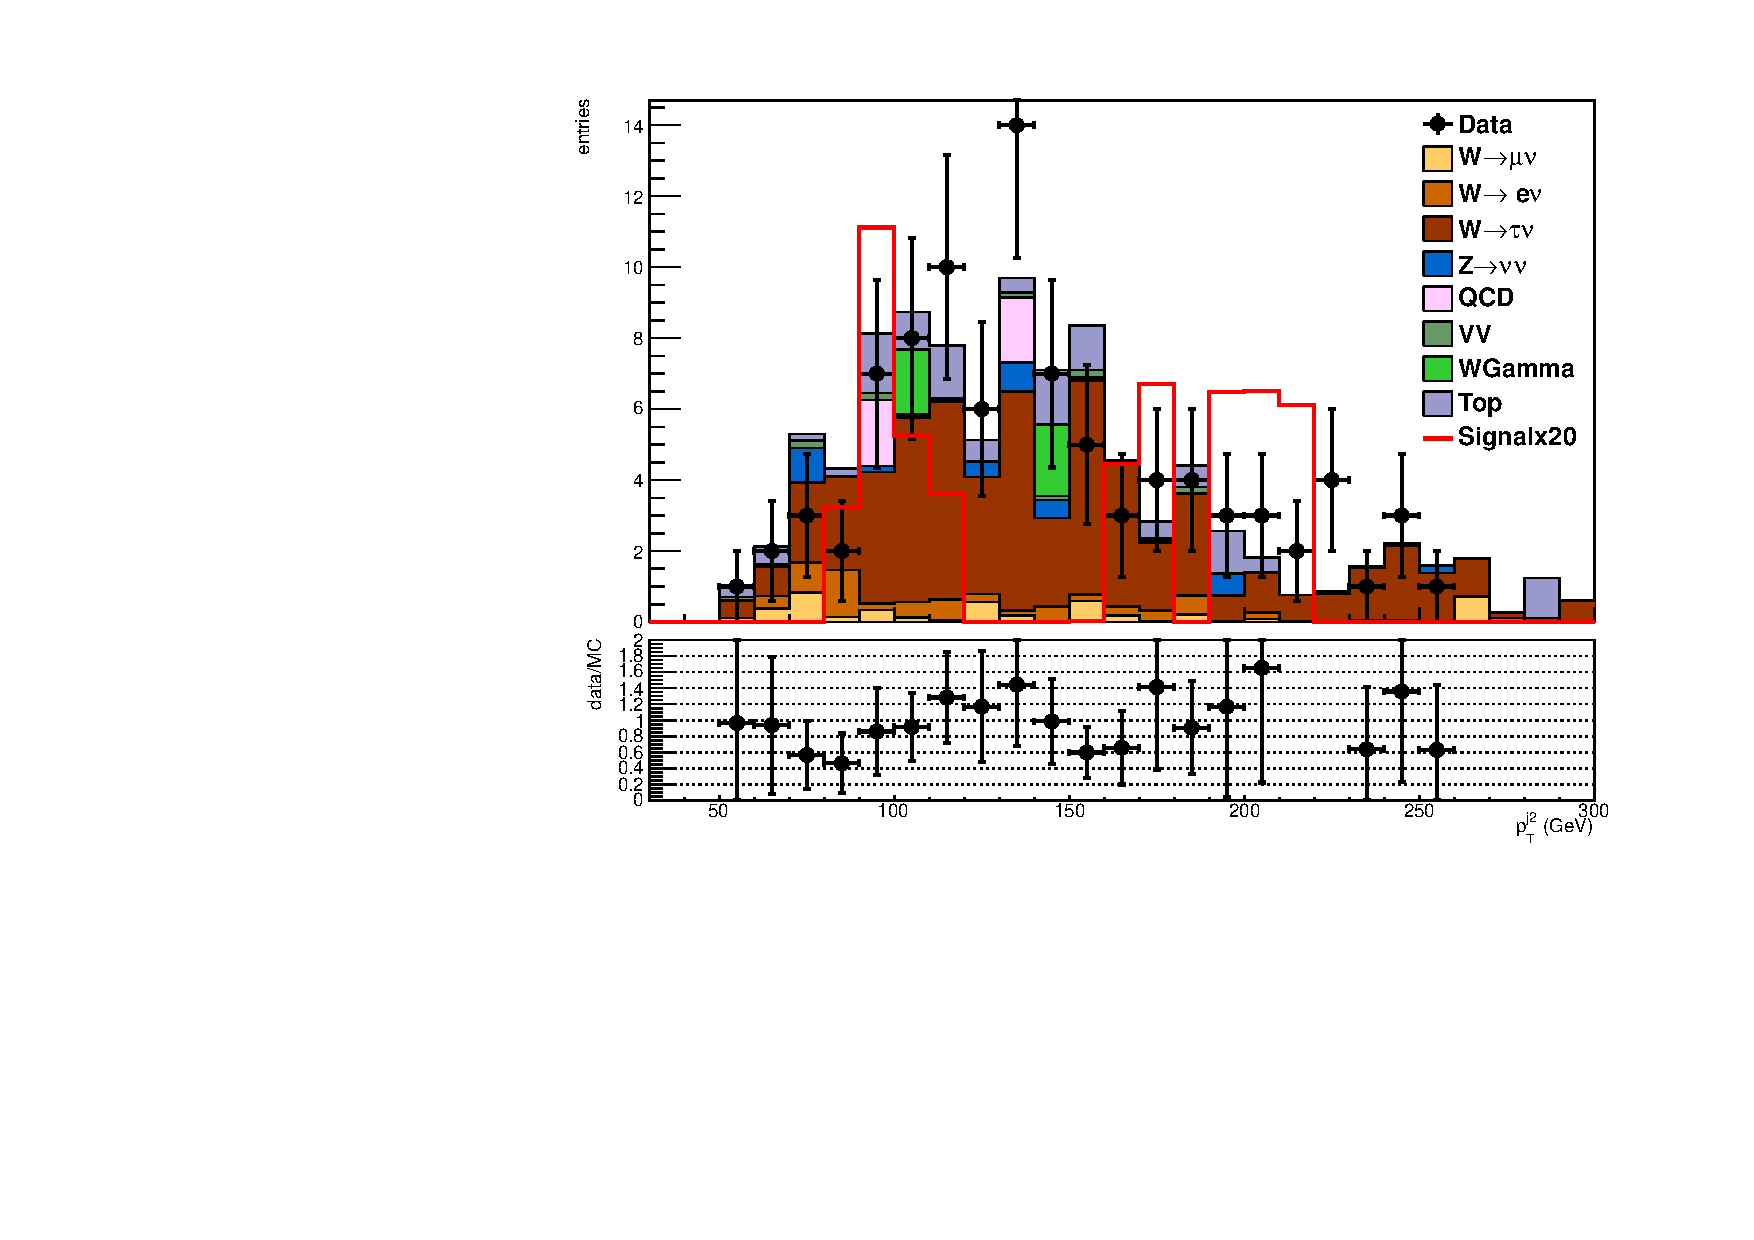
\includegraphics[width=\textwidth]{TalkPics/contplotsandpresel150914/output_contplots_alljetsmetdphicut10/taunu_jet1_pt.pdf}
    \end{block}
    \column{.5\textwidth}
    \begin{block}{Jet 2 pt}
      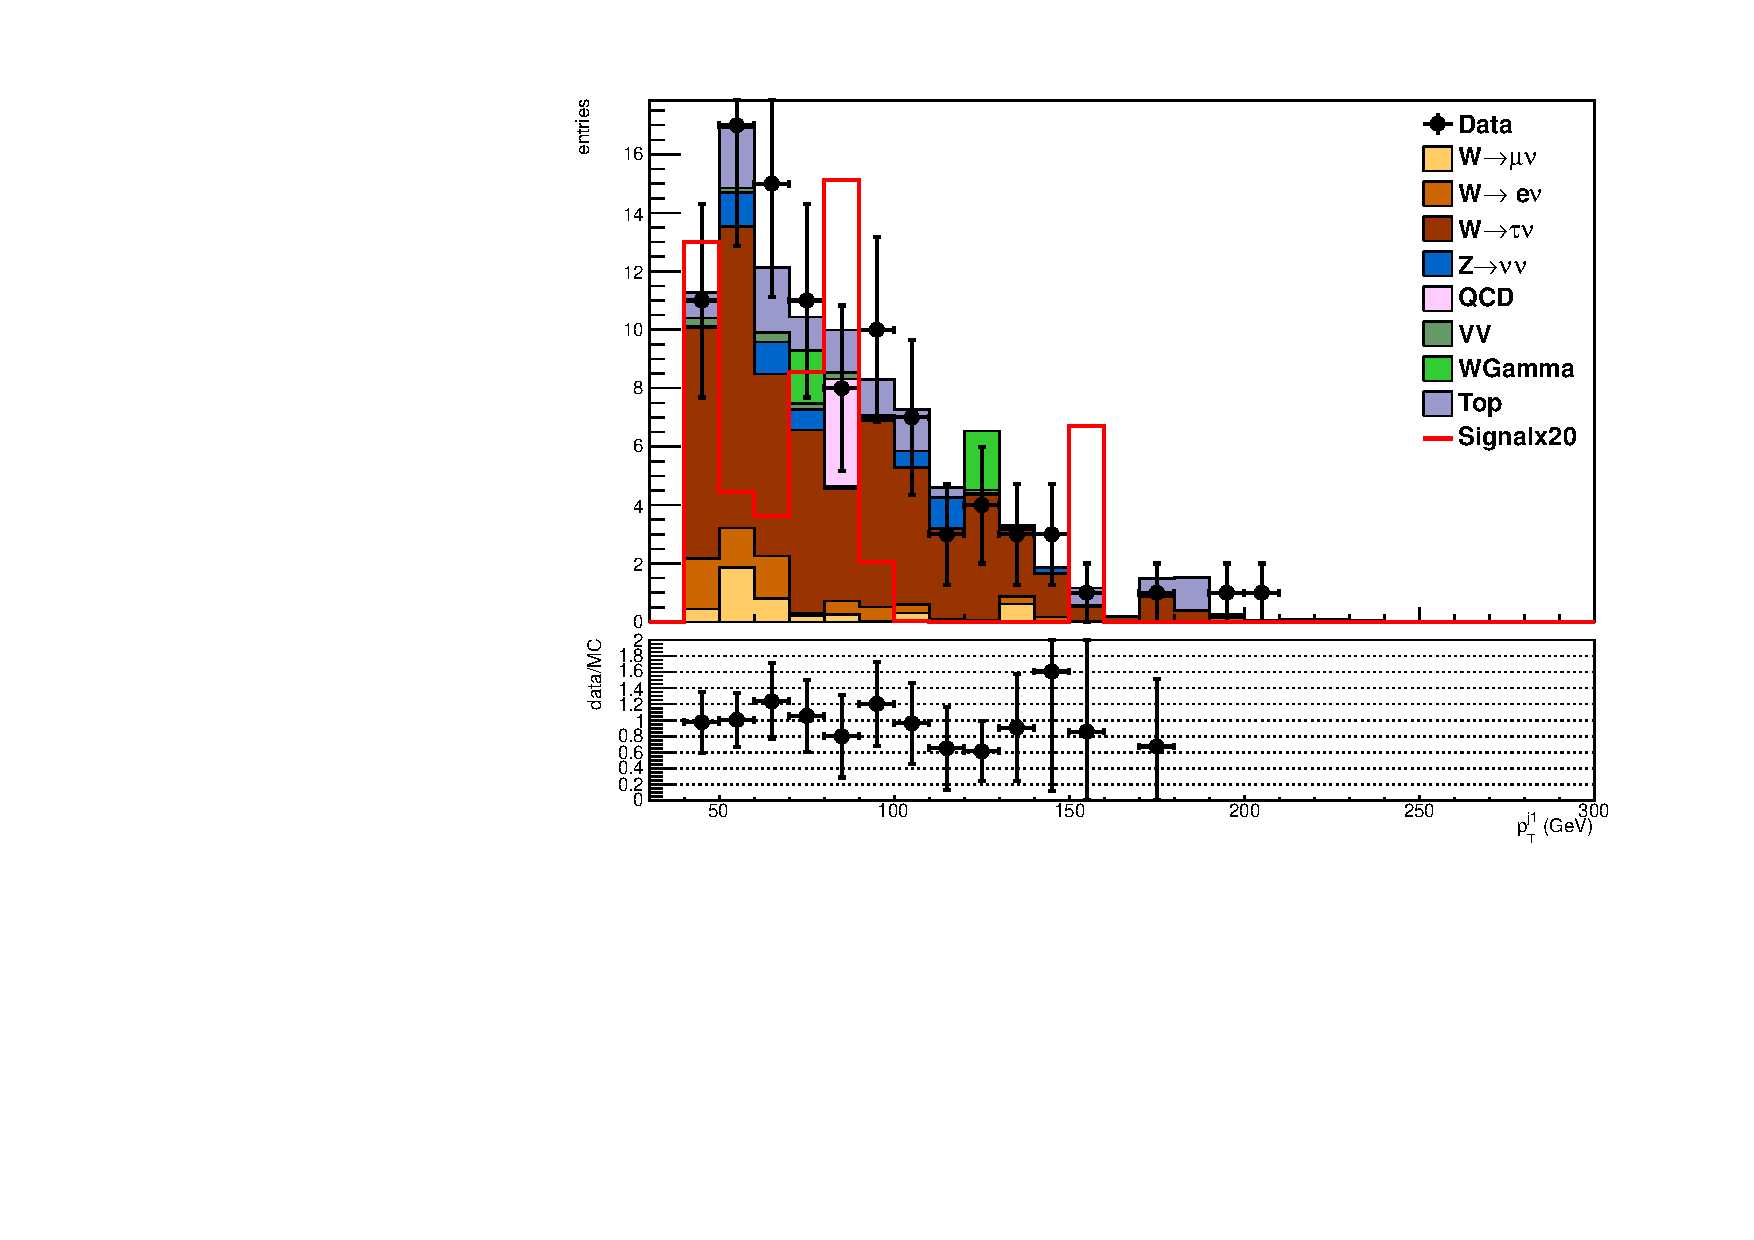
\includegraphics[width=\textwidth]{TalkPics/contplotsandpresel150914/output_contplots_alljetsmetdphicut10/taunu_jet2_pt.pdf}
    \end{block}

  \end{columns}
\end{frame}

\begin{frame}
  \frametitle{New control plots - taunu}
  \begin{columns}
    \column{.5\textwidth}
    \begin{block}{METnomu}
      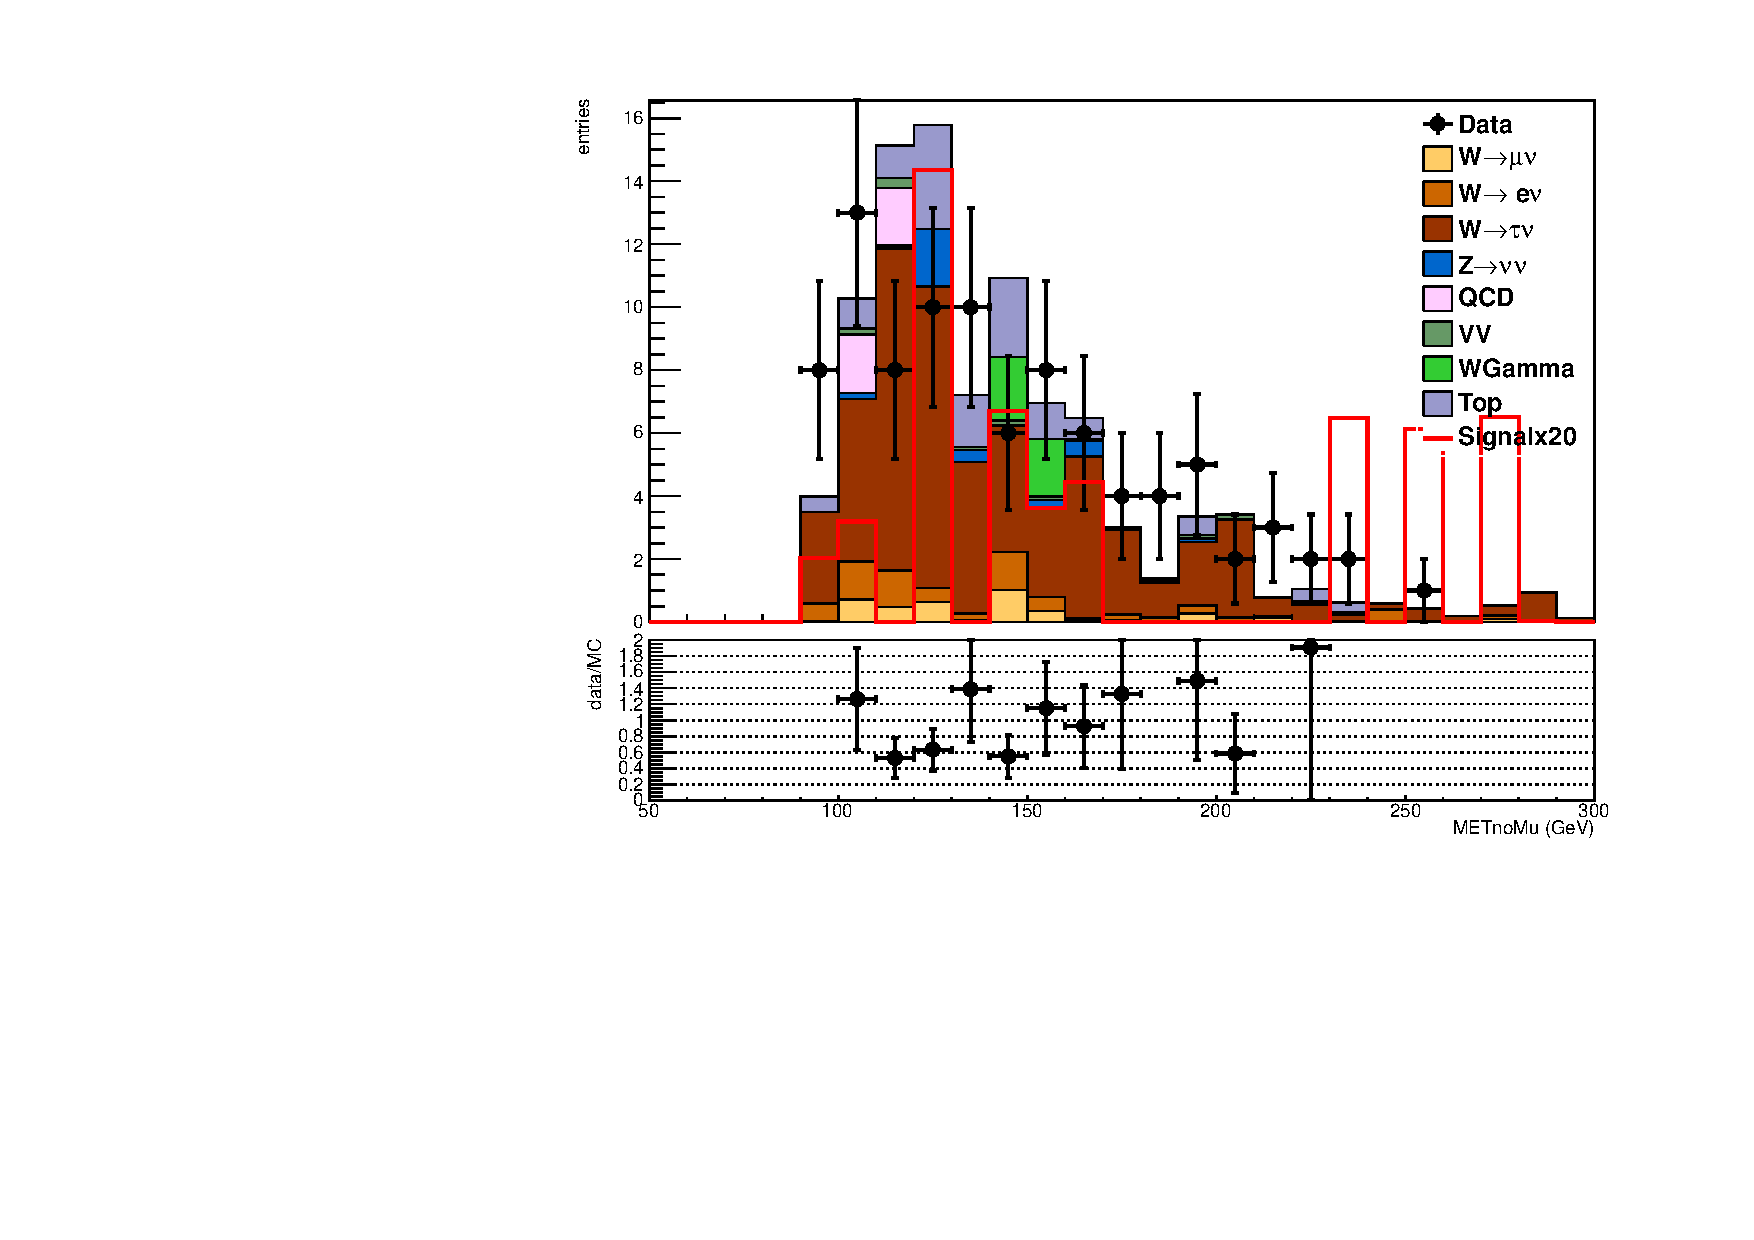
\includegraphics[width=\textwidth]{TalkPics/contplotsandpresel150914/output_contplots_alljetsmetdphicut10/taunu_metnomuons.pdf}
    \end{block}
    \column{.5\textwidth}
    \begin{block}{METnomusig}
      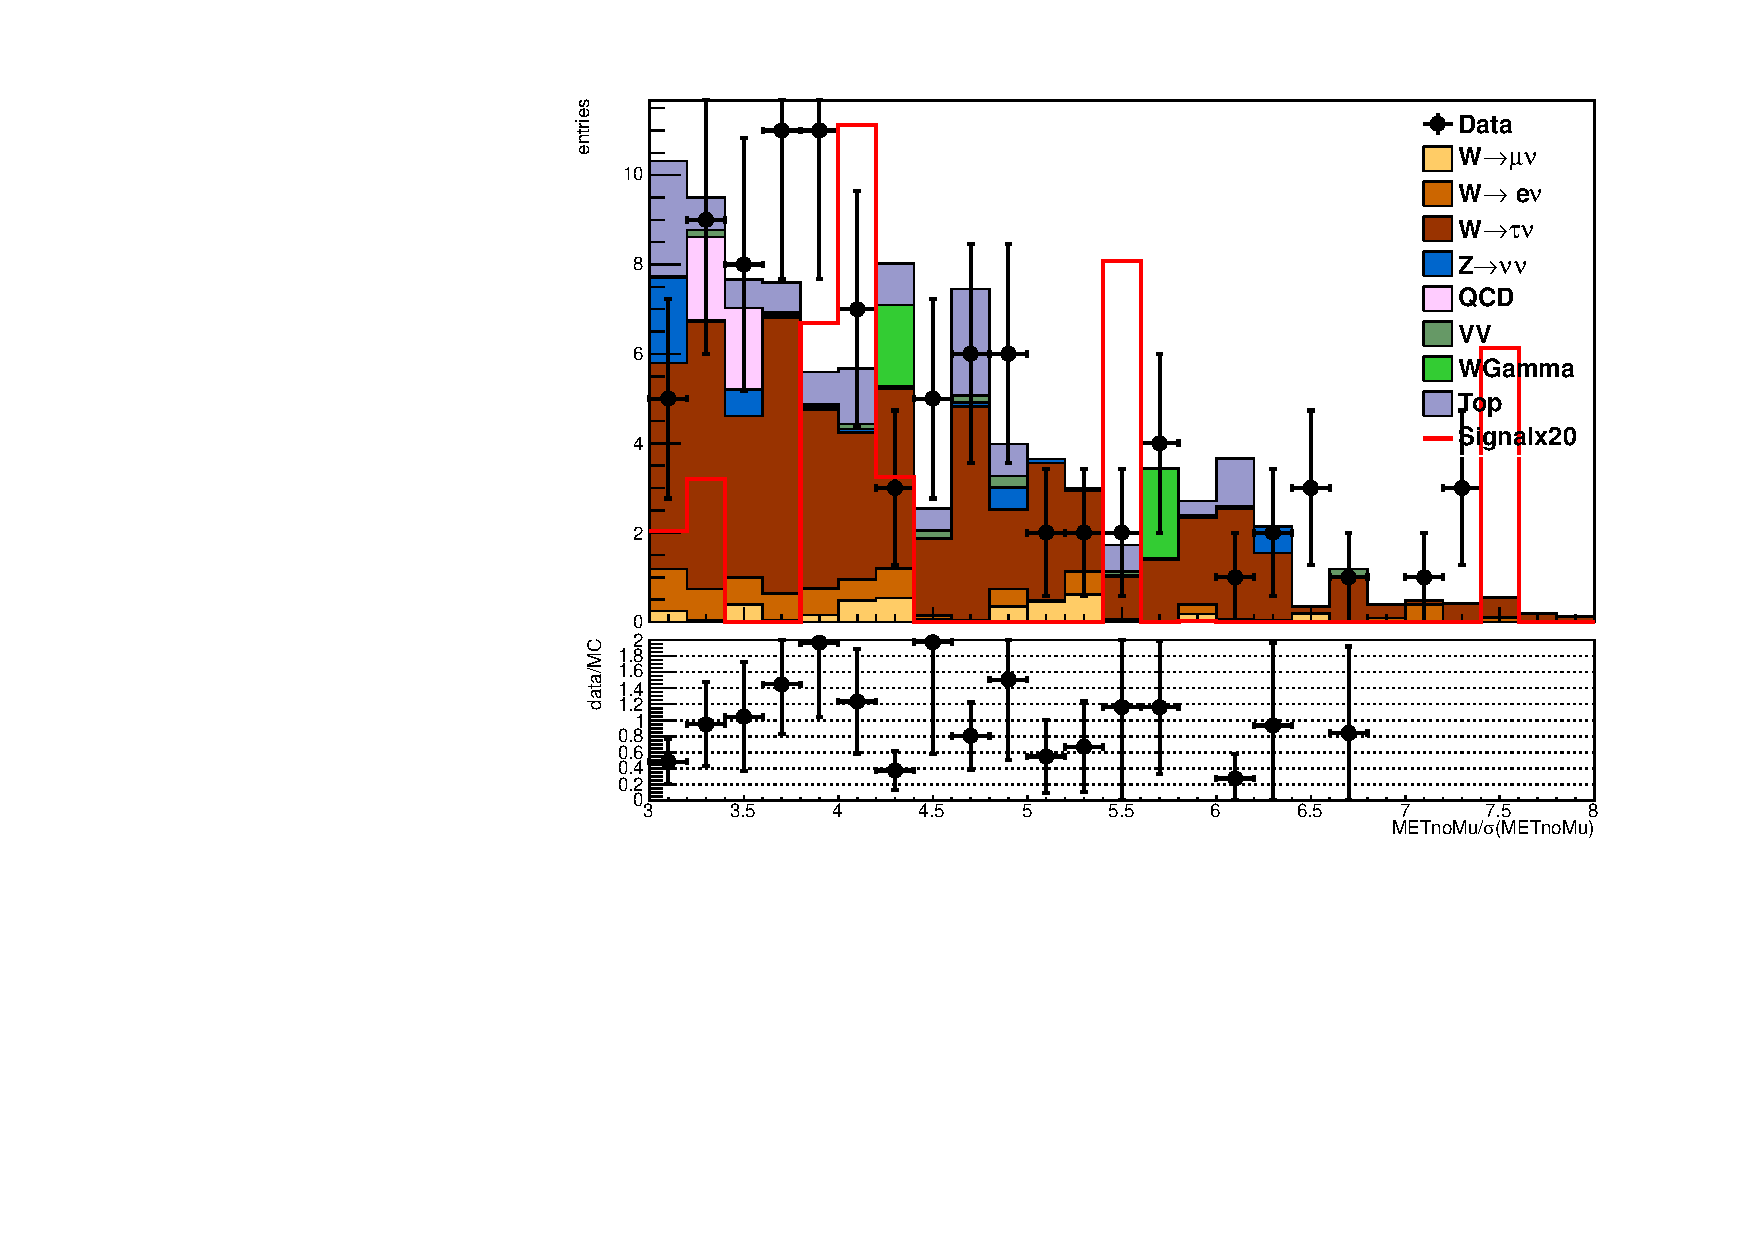
\includegraphics[width=\textwidth]{TalkPics/contplotsandpresel150914/output_contplots_alljetsmetdphicut10/taunu_metnomu_significance.pdf}
    \end{block}

  \end{columns}
\end{frame}

\begin{frame}
  \frametitle{New control plots - taunu}
  \begin{columns}
    \column{.5\textwidth}
    \begin{block}{Mjj}
      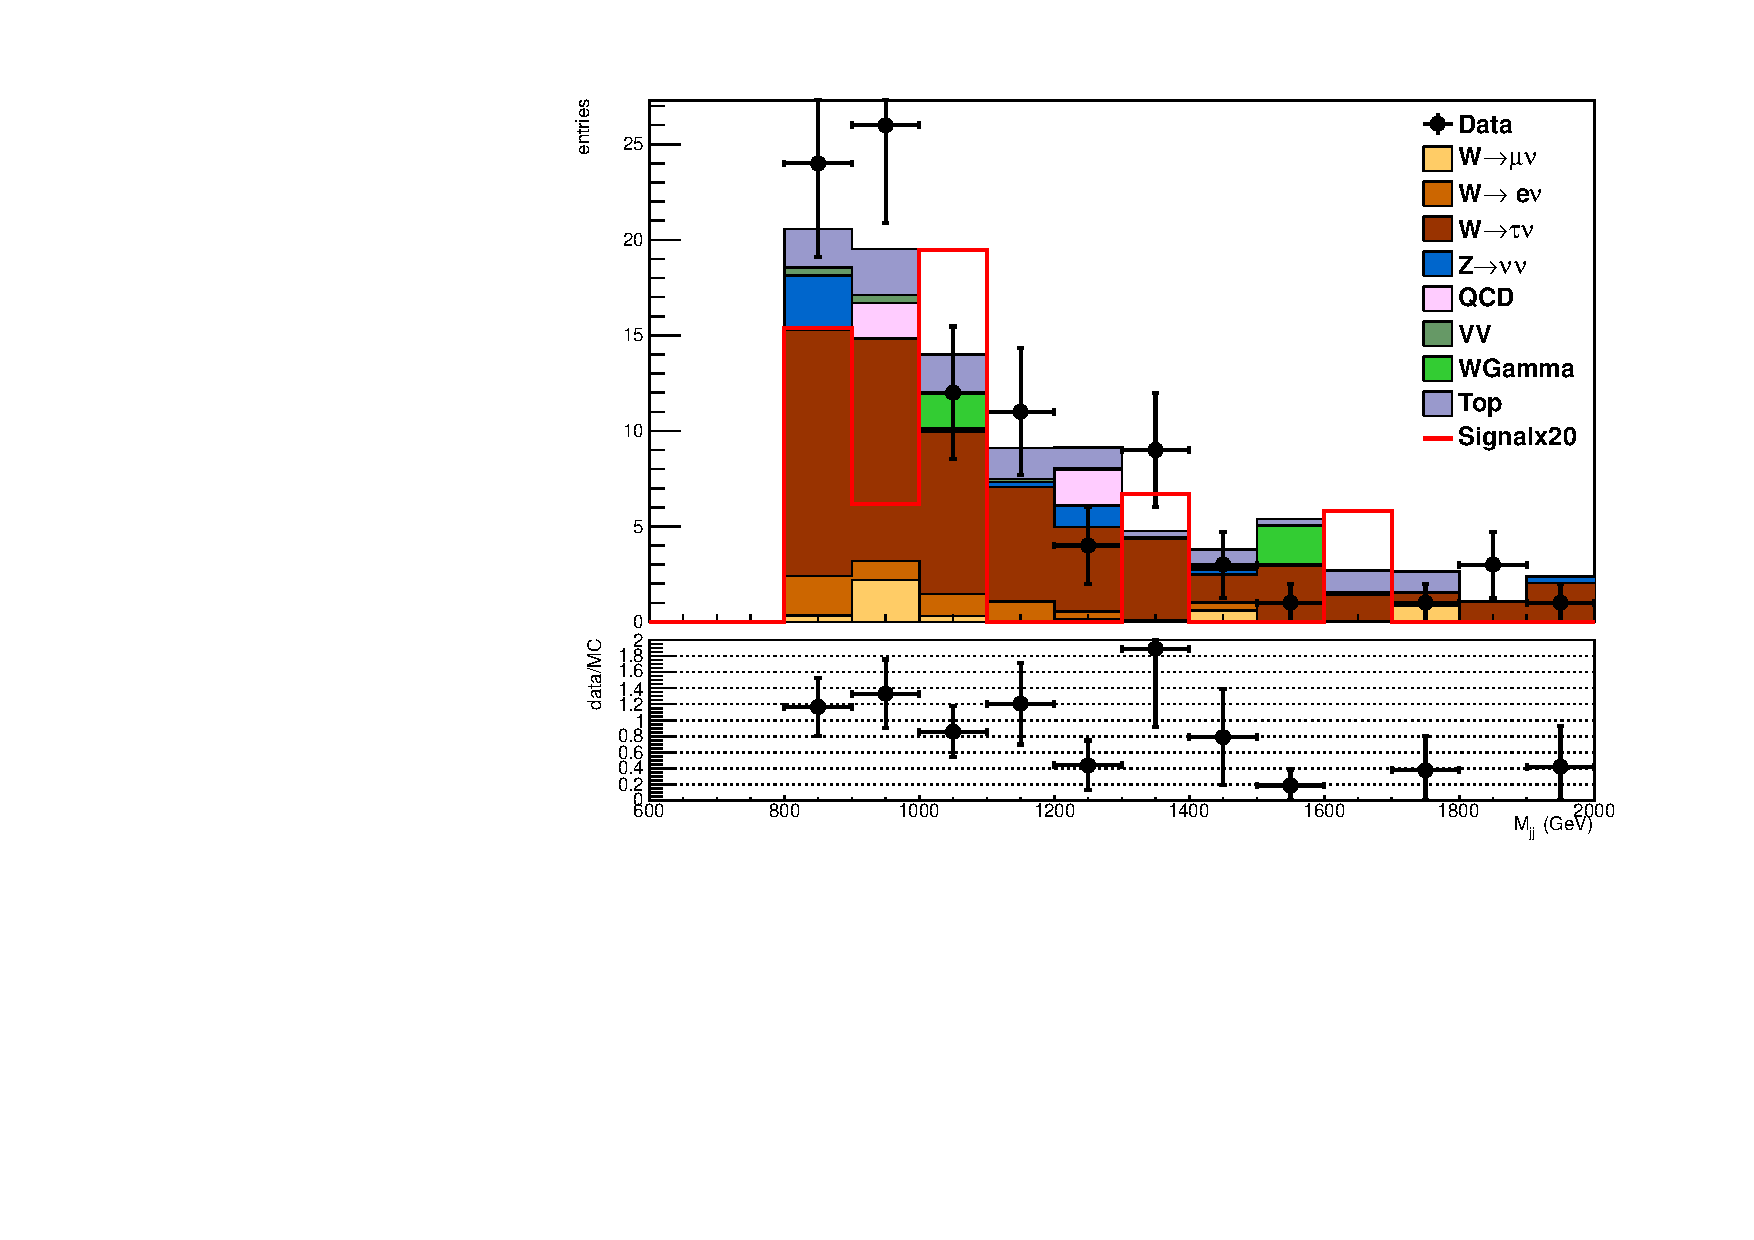
\includegraphics[width=\textwidth]{TalkPics/contplotsandpresel150914/output_contplots_alljetsmetdphicut10/taunu_dijet_M.pdf}
    \end{block}
    \column{.5\textwidth}
    \begin{block}{mt}
      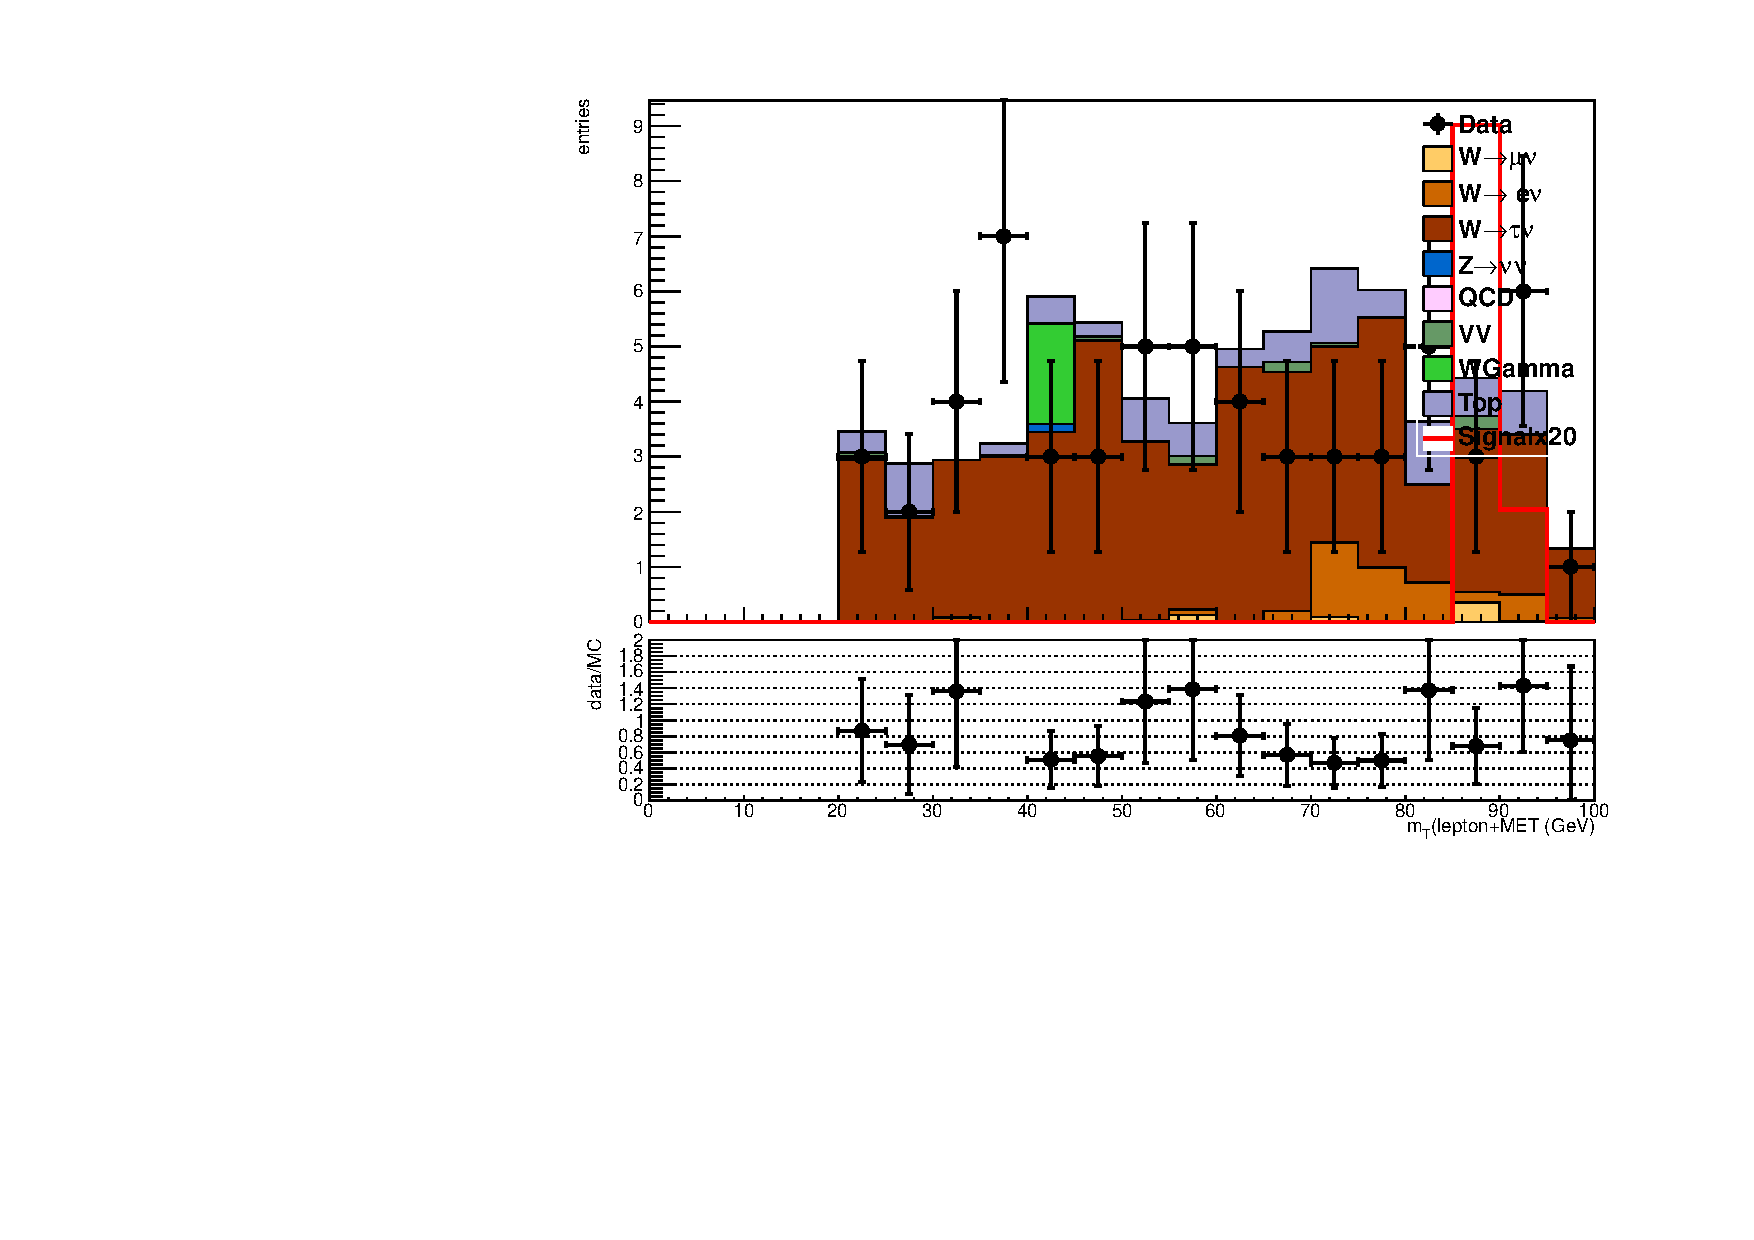
\includegraphics[width=\textwidth]{TalkPics/contplotsandpresel150914/output_contplots_alljetsmetdphicut10/taunu_lep_mt.pdf}
    \end{block}
  \end{columns}
\end{frame}

\begin{frame}
  \frametitle{New control plots - taunu}
  \begin{columns}
    \column{.5\textwidth}
    \begin{block}{Dijet Dphi}
      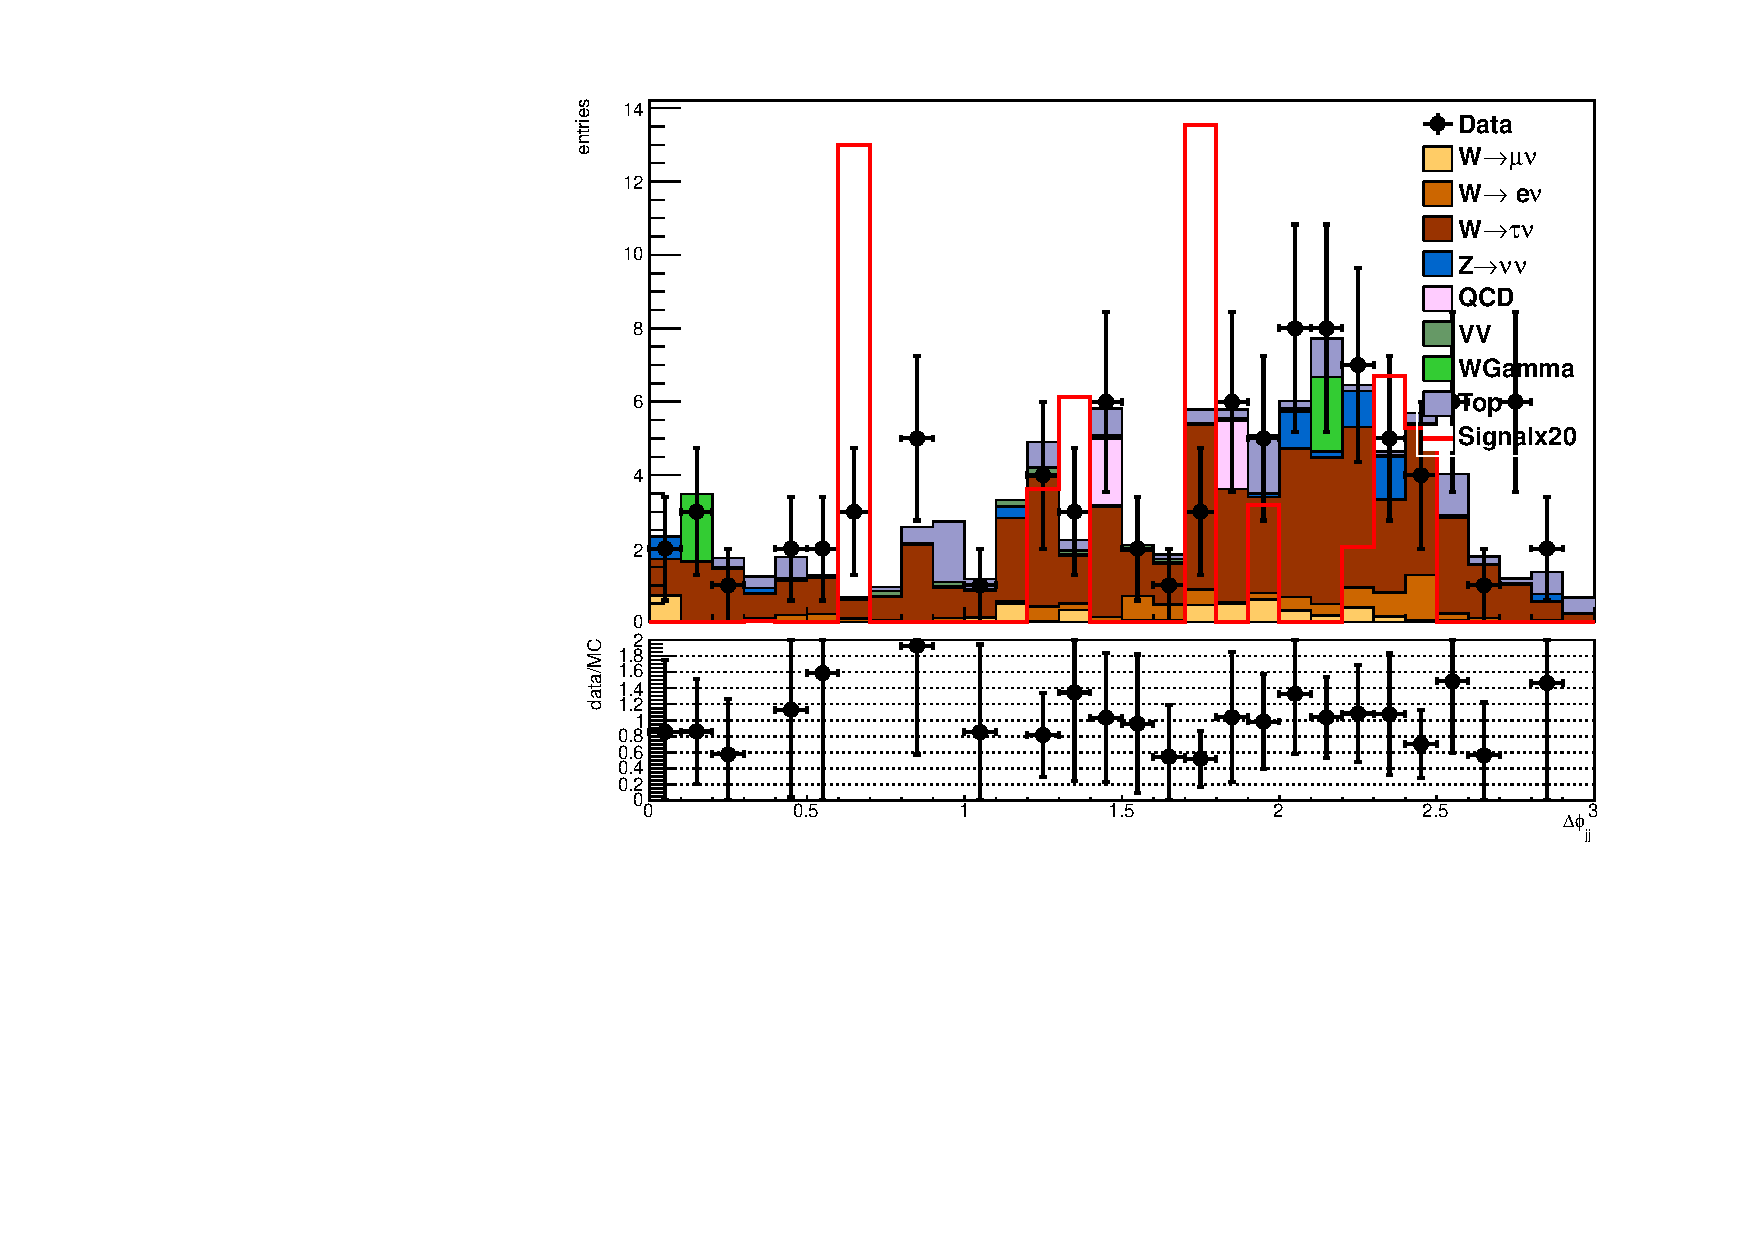
\includegraphics[width=\textwidth]{TalkPics/contplotsandpresel150914/output_contplots_alljetsmetdphicut10/taunu_dijet_dphi.pdf}
    \end{block}
    \column{.5\textwidth}
    \begin{block}{Detajj}
      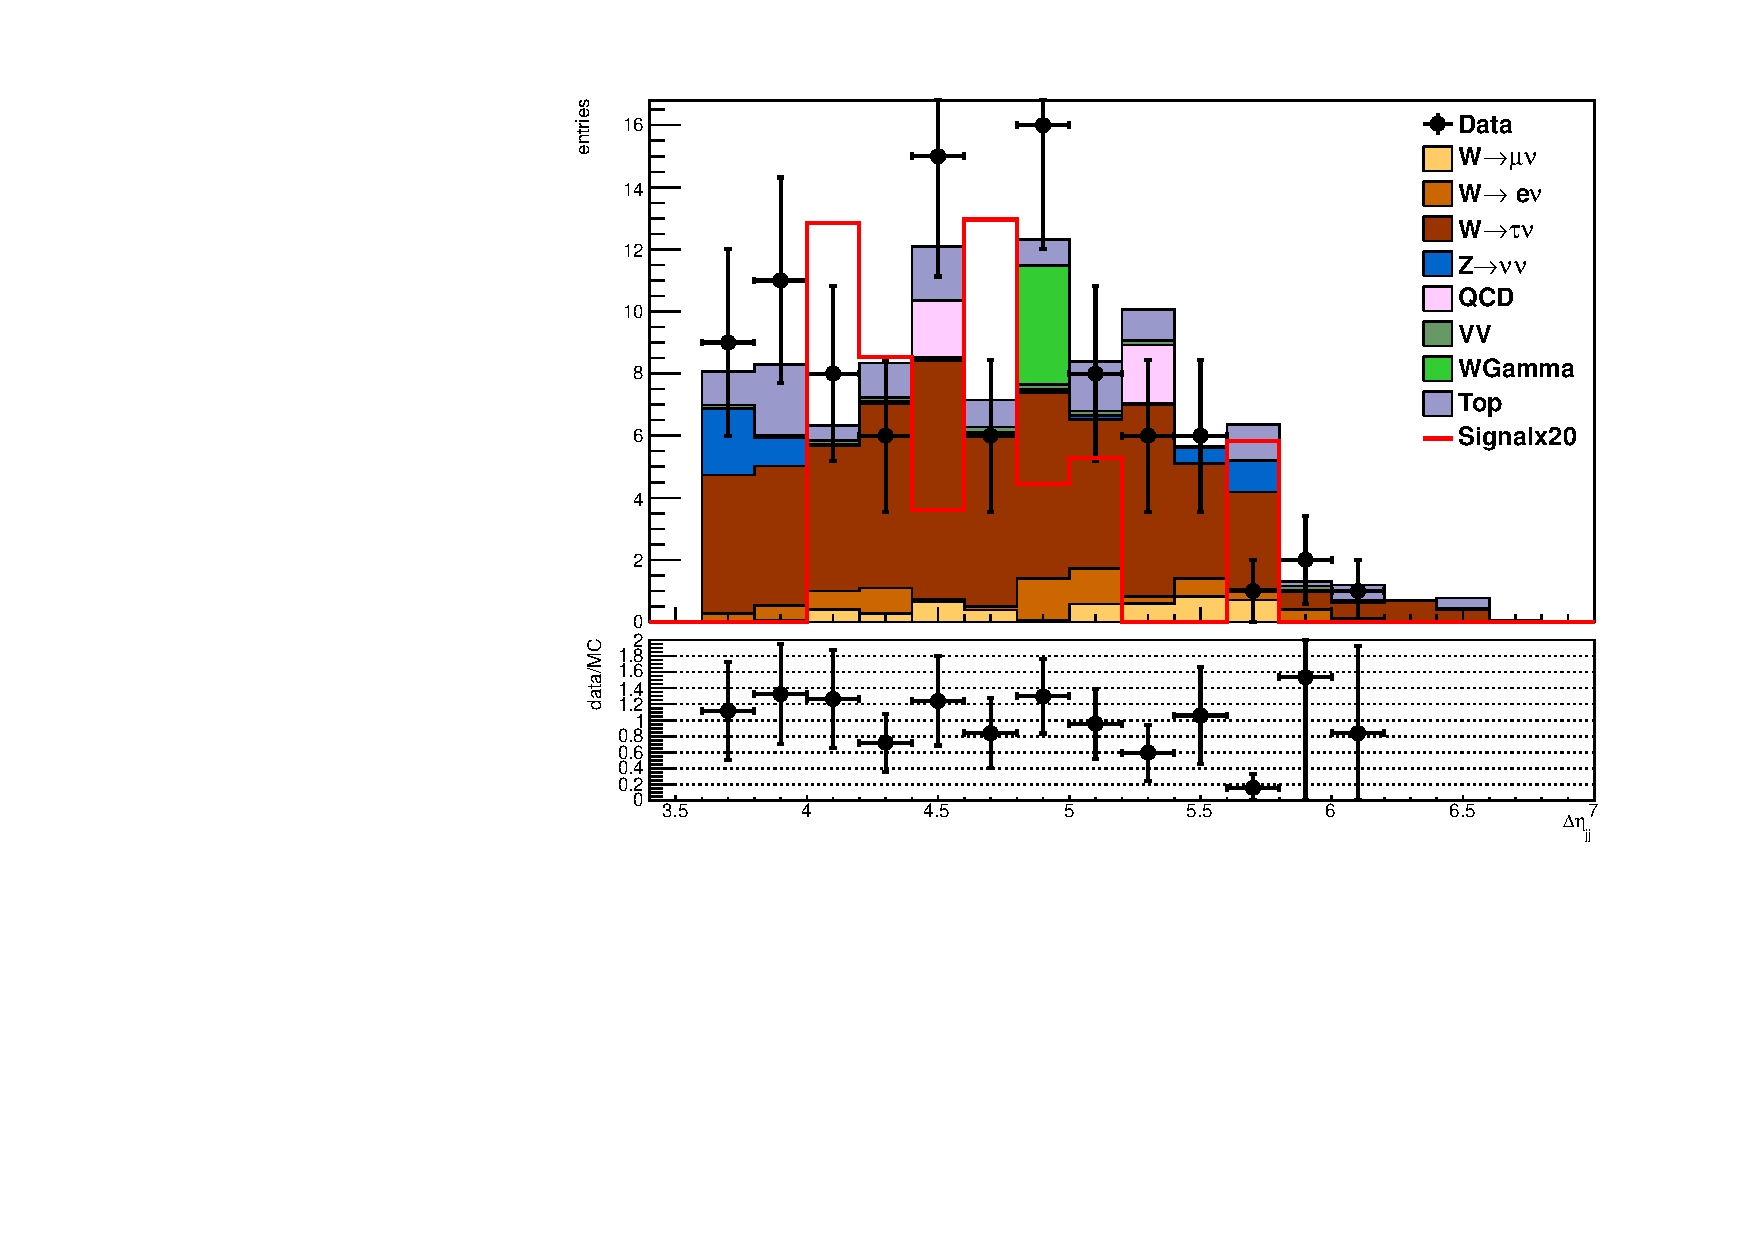
\includegraphics[width=\textwidth]{TalkPics/contplotsandpresel150914/output_contplots_alljetsmetdphicut10/taunu_dijet_deta.pdf}
    \end{block}

  \end{columns}
\end{frame}

\begin{frame}
  \frametitle{New control plots - taunu}
  \begin{columns}
    \column{.5\textwidth}
    \begin{block}{Leading jets-met mindphi}
      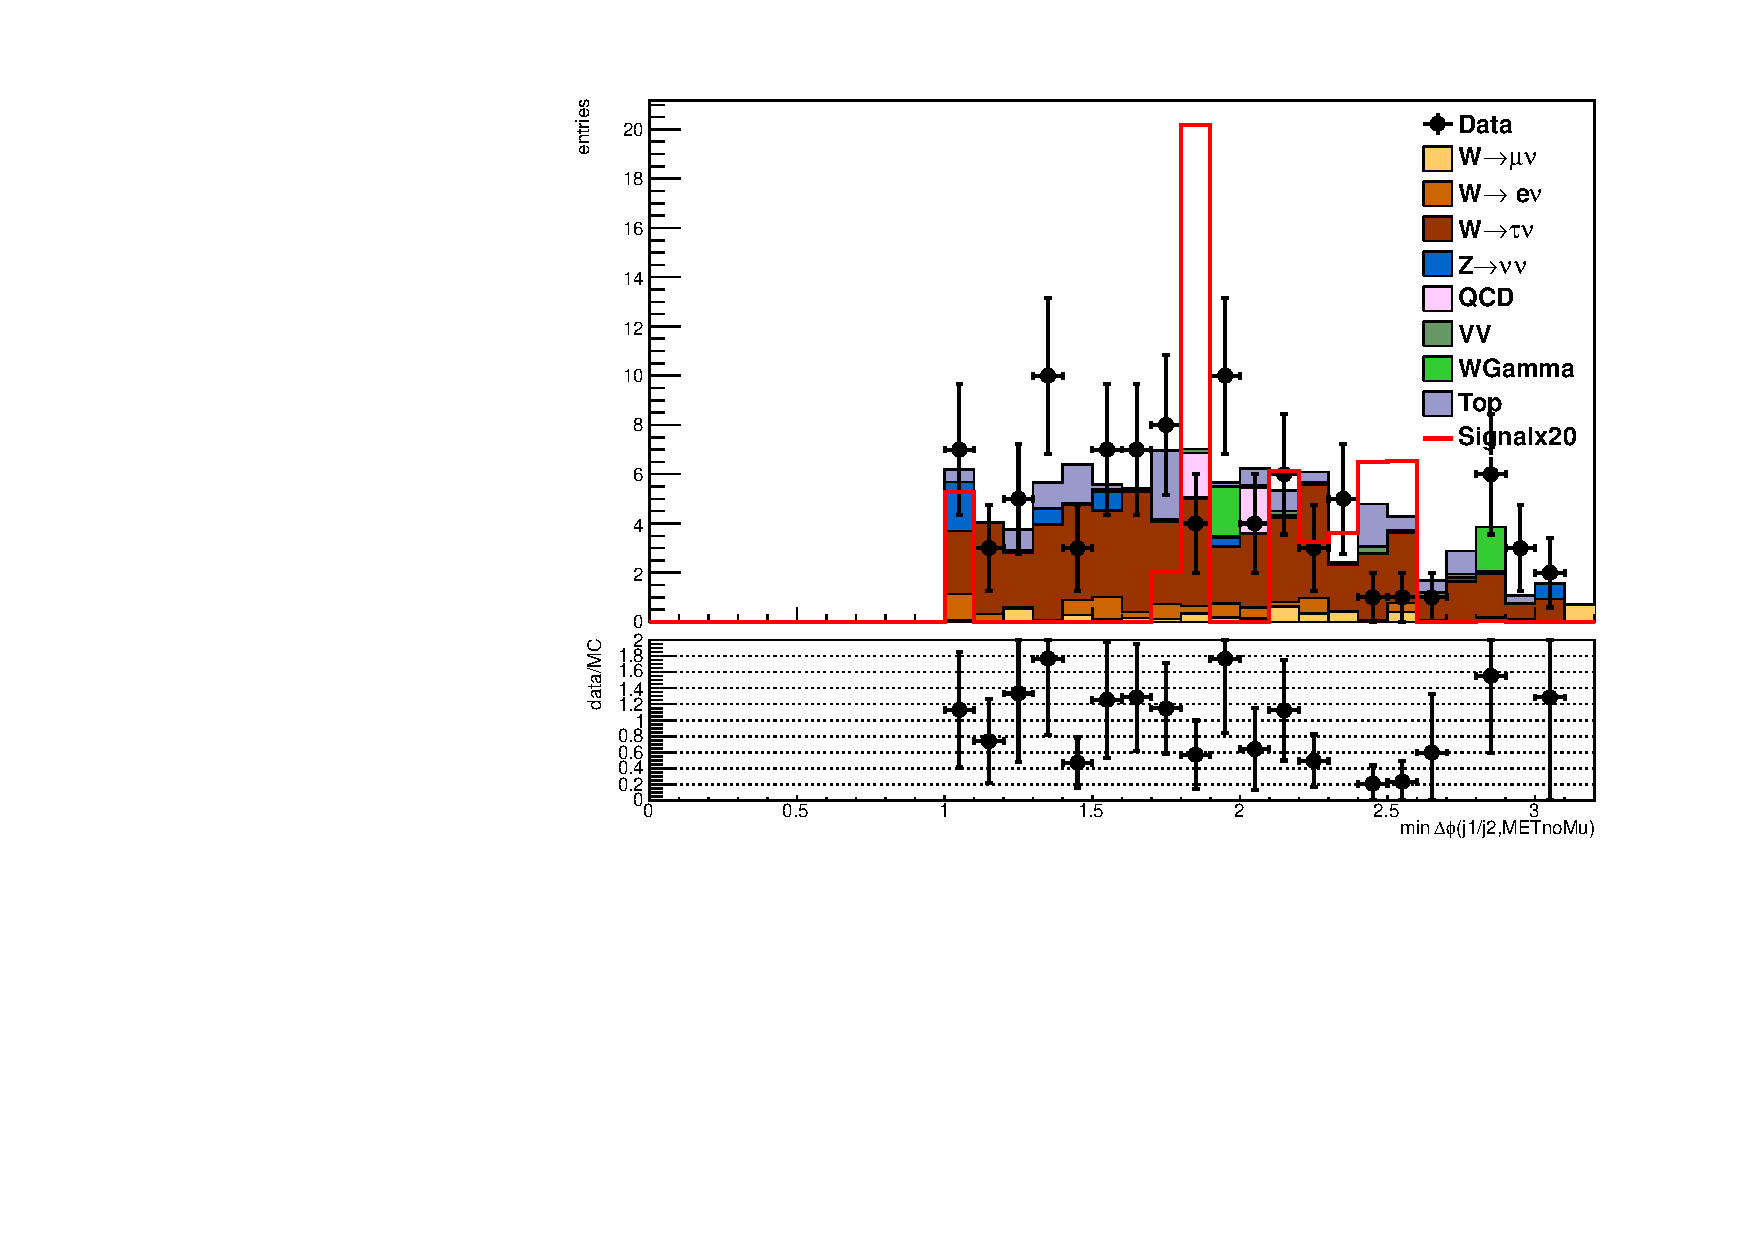
\includegraphics[width=\textwidth]{TalkPics/contplotsandpresel150914/output_contplots_alljetsmetdphicut10/taunu_jetmetnomu_mindphi.pdf}
    \end{block}
    \column{.5\textwidth}
    \begin{block}{All jets-met mindphi}
      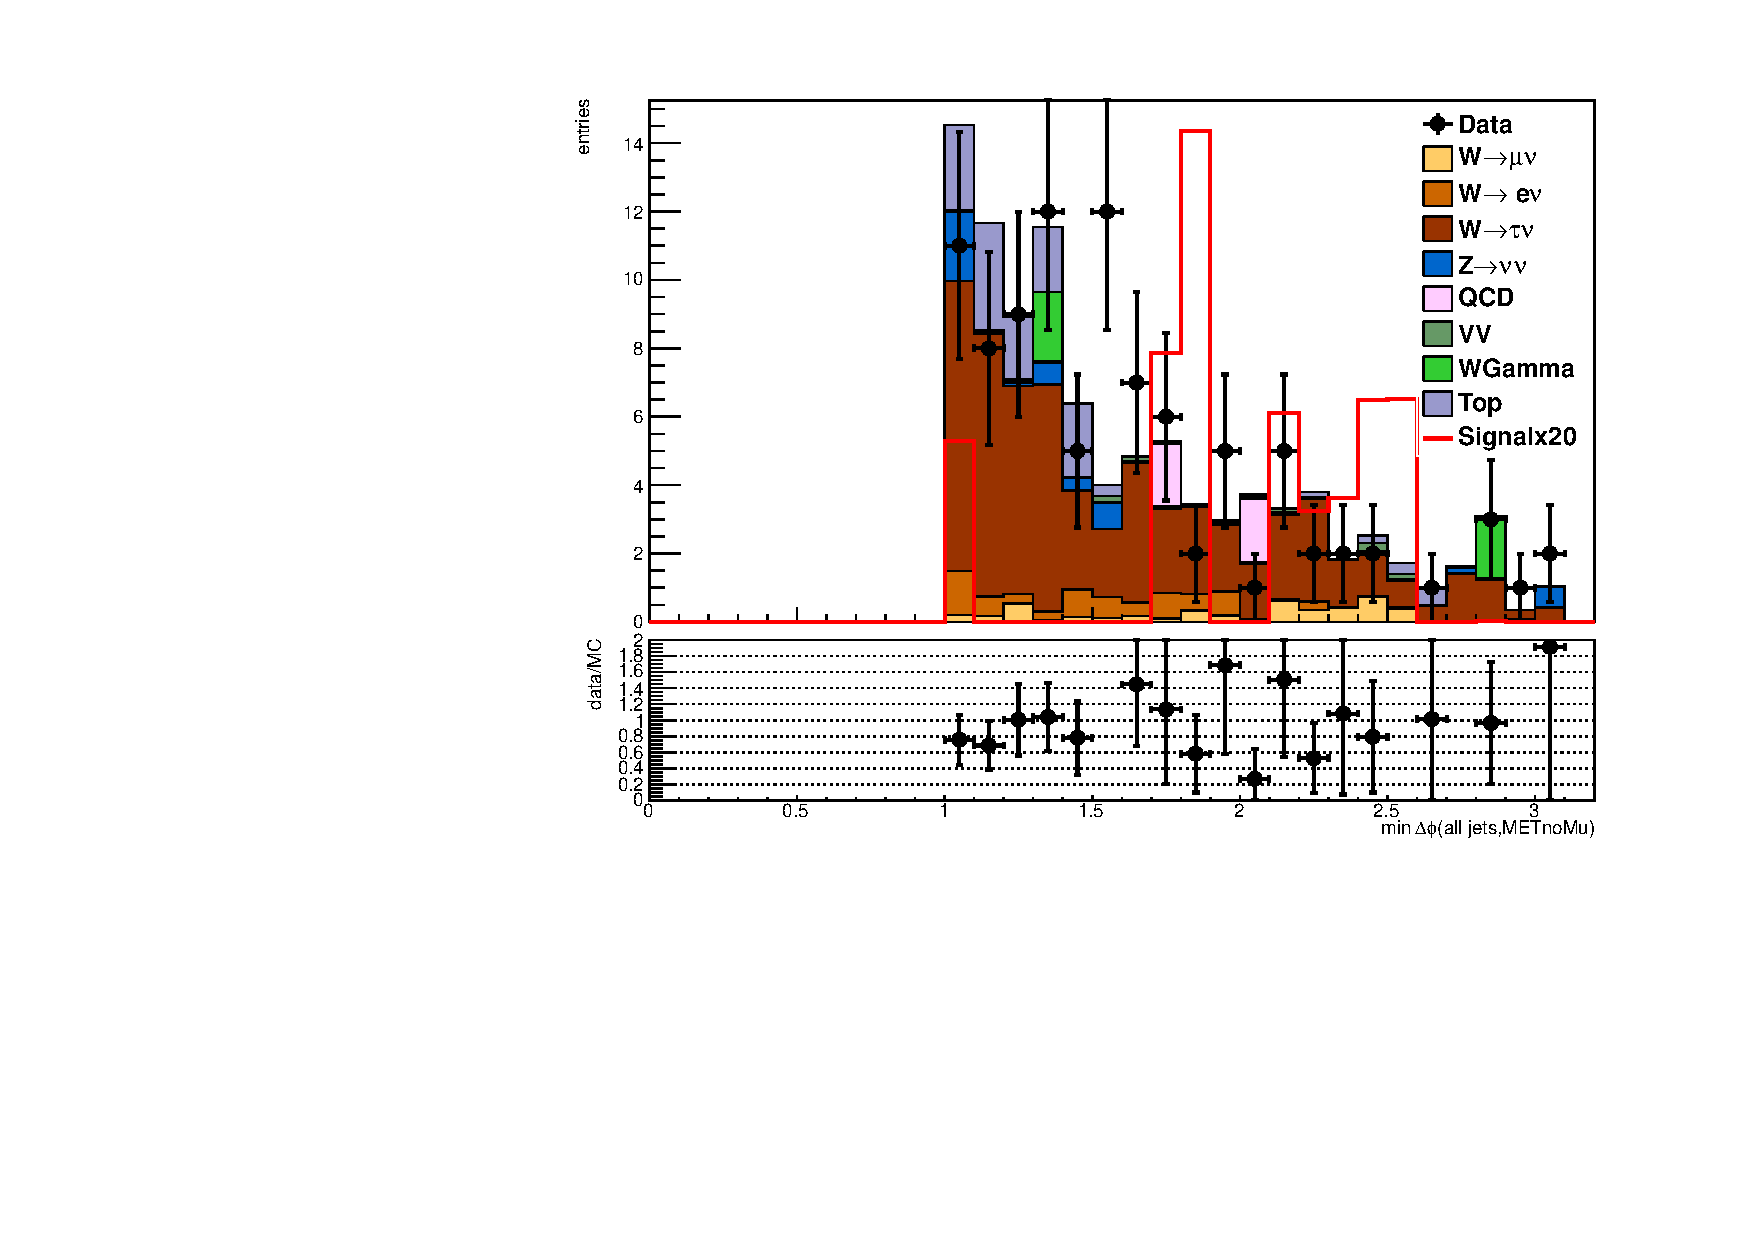
\includegraphics[width=\textwidth]{TalkPics/contplotsandpresel150914/output_contplots_alljetsmetdphicut10/taunu_alljetsmetnomu_mindphi.pdf}
    \end{block}

  \end{columns}
\end{frame}

\begin{frame}
  \frametitle{New control plots - taunu}
  \begin{columns}
    \column{.5\textwidth}
    \begin{block}{dijet-metnomu pt fraction}
      \includegraphics[width=\textwidth]{TalkPics/contplotsandpresel150914/output_contplots_alljetsmetdphicut10/taunu_dijetmetnomu_ptfraction.pdf}
    \end{block}
  \end{columns}
\end{frame}

\begin{frame}
  \frametitle{New control plots - sig}
  \begin{columns}
    \column{.5\textwidth}
    \begin{block}{Jet 1 pt}
      \includegraphics[width=\textwidth]{TalkPics/contplotsandpresel150914/output_contplots_alljetsmetdphicut10/nunu_jet1_pt.pdf}
    \end{block}
    \column{.5\textwidth}
    \begin{block}{Jet 2 pt}
      \includegraphics[width=\textwidth]{TalkPics/contplotsandpresel150914/output_contplots_alljetsmetdphicut10/nunu_jet2_pt.pdf}
    \end{block}

  \end{columns}
\end{frame}

\begin{frame}
  \frametitle{New control plots - sig}
  \begin{columns}
    \column{.5\textwidth}
    \begin{block}{METnomu}
      \includegraphics[width=\textwidth]{TalkPics/contplotsandpresel150914/output_contplots_alljetsmetdphicut10/nunu_metnomuons.pdf}
    \end{block}
    \column{.5\textwidth}
    \begin{block}{METnomusig}
      \includegraphics[width=\textwidth]{TalkPics/contplotsandpresel150914/output_contplots_alljetsmetdphicut10/nunu_metnomu_significance.pdf}
    \end{block}

  \end{columns}
\end{frame}

\begin{frame}
  \frametitle{New control plots - sig}
  \begin{columns}
    \column{.5\textwidth}
    \begin{block}{Mjj}
      \includegraphics[width=\textwidth]{TalkPics/contplotsandpresel150914/output_contplots_alljetsmetdphicut10/nunu_dijet_M.pdf}
    \end{block}
    \column{.5\textwidth}
  \end{columns}
\end{frame}

\begin{frame}
  \frametitle{New control plots - sig }
  \begin{columns}
    \column{.5\textwidth}
    \begin{block}{Dijet Dphi}
      \includegraphics[width=\textwidth]{TalkPics/contplotsandpresel150914/output_contplots_alljetsmetdphicut10/nunu_dijet_dphi.pdf}
    \end{block}
    \column{.5\textwidth}
    \begin{block}{Detajj}
      \includegraphics[width=\textwidth]{TalkPics/contplotsandpresel150914/output_contplots_alljetsmetdphicut10/nunu_dijet_deta.pdf}
    \end{block}

  \end{columns}
\end{frame}

\begin{frame}
  \frametitle{New control plots - sig}
  \begin{columns}
    \column{.5\textwidth}
    \begin{block}{Leading jets-met mindphi}
      \includegraphics[width=\textwidth]{TalkPics/contplotsandpresel150914/output_contplots_alljetsmetdphicut10/nunu_jetmetnomu_mindphi.pdf}
    \end{block}
    \column{.5\textwidth}
    \begin{block}{All jets-met mindphi}
      \includegraphics[width=\textwidth]{TalkPics/contplotsandpresel150914/output_contplots_alljetsmetdphicut10/nunu_alljetsmetnomu_mindphi.pdf}
    \end{block}

  \end{columns}
\end{frame}

\begin{frame}
  \frametitle{New control plots - sig}
  \begin{columns}
    \column{.5\textwidth}
    \begin{block}{dijet-metnomu pt fraction}
      \includegraphics[width=\textwidth]{TalkPics/contplotsandpresel150914/output_contplots_alljetsmetdphicut10/nunu_dijetmetnomu_ptfraction.pdf}
    \end{block}
  \end{columns}
\end{frame}


\begin{frame}
  \frametitle{Conclusions}
  \label{lastframe}

  \begin{block}{}
    \scriptsize
    \begin{itemize}
    \item Focused on agreement in control regions
    \item[-] This minimises effect of mismodelled QCD
    \item New pre-selection proposed:
    \item $m_{T}$ cut added to taunu to reduce QCD
    \item[-] could consider also adding to munu region
    \item Added all jets-met $\Delta\phi$ cut
    \item[-] Significant improvement over leading jets-met $\Delta\phi$ cut
    \end{itemize}
  \end{block}

\end{frame}

\begin{frame}
  \frametitle{Backup}
\end{frame}

\end{fmffile}
\end{document}
